\chapter{Stationary black holes}
\label{s:sta}\index{stationary!black hole}

\minitoc

\section{Introduction}

Having defined black holes in all generality in Chap.~\ref{s:glo}, we focus
here on the steady state case, i.e. black holes in stationary spacetimes.
We have already discussed
non-expanding horizons and Killing horizons in Chap.~\ref{s:neh} as
possible models for the event horizon of a
steady state black hole. Actually, we shall see below that (each connected
component of) the event horizon of a black hole in a stationary spacetime has to be
a Killing horizon, at least in the framework of general relativity and within
rather general hypotheses.
We shall start by defining properly the concept of a stationary
spacetime and investigating some first properties of a black hole
in such a spacetime (Sec.~\ref{s:sta:sta_st}).
Then, in Sec.~\ref{s:sta:mass_angul_mom}, we discuss the concepts
of mass and angular momentum in asymptotically flat spacetimes, which are useful to characterize black holes. In Sec.~\ref{s:sta:EH_KH}, we shall
see that
if the Killing vector $\w{\xi}$ generating stationarity is null on
a connected event horizon $\Hor$, the latter is a Killing horizon with
respect to $\w{\xi}$.  If $\Hor$ is non-degenerate and the
electrovacuum Einstein equation holds, this can only occur in a static spacetime
(\emph{staticity theorem}, Sec.~\ref{s:sta:staticity_thm}).
On the contrary, if $\w{\xi}$ is spacelike\footnote{The timelike
case is excluded for an event horizon is a null hypersurface.} on some parts of $\Hor$, then, modulo the
electrovacuum Einstein equation and some additional hypotheses,
$\Hor$ is still a Killing horizon, albeit with respect to a Killing vector
distinct from $\w{\xi}$ (\emph{strong rigidity theorem}, Sec.~\ref{s:sta:strong_rigidity}).
Section~\ref{s:sta:Smarr} is devoted to an important relation between various global
quantities characterizing a stationary black hole: the \emph{Smarr formula}.
This is the opportunity to investigate electromagnetic
fields on the horizon of a stationary black hole, in particular to define
the black hole's electric charge and electric potential, both of them being involved
in the Smarr formula. The culmination point of this chapter is
Sec.~\ref{s:sta:no-hair}, which presents the famous
\emph{no-hair theorem}. Modulo some hypotheses, this theorem stipulates that in 4-dimensional
general relativity, all isolated stationary electrovacuum black holes are necessarily
Kerr-Newman black holes; in the pure vacuum case (the most relevant one for astrophysics),
they are Kerr black holes, to be explored in Part.~\ref{P:ker}.

\section{Stationary spacetimes} \label{s:sta:sta_st}

\subsection{Definitions} \label{s:sta:def_station}

\begin{greybox}
A spacetime $(\M,\w{g})$ is called \defin{stationary}\index{stationary!spacetime}
iff (i) it is invariant under
the action of the translation group $(\R,+)$ and (ii) the orbits of
the group action (cf. Sec.~\ref{s:neh:symmetries})
are everywhere timelike curves or (ii') $(\M,\w{g})$
admits a conformal completion (cf. Sec.~\ref{s:glo:conf_compl})
and the orbits of the group action are timelike in the vicinity of
the conformal boundary $\scri$.
It is equivalent to say that there exists a Killing vector field
$\w{\xi}$ (the generator of the translation group, cf. Sec.~\ref{s:neh:symmetries}) that is
timelike everywhere or at least in the vicinity of $\scri$ when there exists a conformal
completion. We shall say that $(\M,\w{g})$ is \defin{strictly stationary}\index{strictly!stationary}\index{stationary!strictly --} iff the Killing vector field $\w{\xi}$ is timelike in all $\M$,
i.e. iff property (ii) above is fulfilled.
\end{greybox}

\begin{remark} \label{r:sta:pseudo-stationary}
Some authors (e.g. Carter \cite{Carte73b}) call
\emph{pseudo-stationary}\index{pseudo-stationary} the stationary spacetimes
that obey (ii'), keeping the qualifier
\emph{stationary} for the strictly stationary case.
As we are going to see, when $\M$
contains a black hole, $\w{\xi}$ cannot be timelike everywhere,
so only \emph{pseudo-stationarity} in Carter's sense is relevant for such spacetimes.
Our terminology, namely keeping the qualifier \emph{stationary} even for (ii'),  follows that of
Choquet-Bruhat \cite{Choqu09},
Chru\'sciel, Lopes Costa \& Heusler \cite{ChrusLH12},
Heusler \cite{Heusl96}
and Wald \cite{Wald01}.
\end{remark}

The Killing vector field $\w{\xi}$ is a priori not unique: the translation group $(\R,+)$
admits the reparametrization
$t\mapsto t' = \alpha t$, where $\alpha$ is a nonzero constant, which yields
the rescalling $\w{\xi} \mapsto \w{\xi'} = \alpha^{-1} \w{\xi}$
of the Killing vector field [cf. Eq.~(\ref{e:neh:xi_dxdt})]. When the
spacetime admits a conformal boundary $\scri$ --- which is required if a black hole
is present, given the definition (\ref{e:glo:def_BH}) ---, then
one selects $\w{\xi}$ by demanding that it is future-directed near $\scri$ and
obeys
\be \label{e:sta:xi_scri}
    \w{\xi}\cdot\w{\xi} \to -1 \quad \mbox{near\ } \scri .
\ee
This determines $\w{\xi}$ uniquely, since this fixes
the rescaling constant $\alpha$ to $\pm 1$, with only $+1$ being acceptable
to keep the time orientation.

If the stationary spacetime is endowed with electromagnetic and/or
matter fields, they must respect the stationarity as well. For the electromagnetic
field $\w{F}$ (cf. Sec.~\ref{e:fra:electrovacuum}), this is expressed by
the vanishing of the Lie derivative along $\w{\xi}$:
\be
    \Lie{\xi} \w{F} = 0 .
\ee
This condition is similar to Killing-vector property
$\Lie{\xi} \w{g} = 0$ [Eq.~(\ref{e:neh:Lie_xi_g})].

A notion stronger than stationarity is that of \emph{staticity}:

\begin{greybox}
A spacetime $(\M,\w{g})$ is called \defin{static}\index{static!spacetime}
iff (i) it is stationary and (ii) the Killing vector field $\w{\xi}$
generating the stationary action is orthogonal to a family of hypersurfaces
(one says that $\w{\xi}$ is \defin{hypersurface-orthogonal}\index{hypersurface-orthogonal}).
The spacetime $(\M,\w{g})$ is called \defin{strictly static}\index{strictly!static}\index{static!strictly --}
iff moreover $\w{\xi}$ is timelike in all $\M$.
\end{greybox}

\begin{remark}
The same comment as in Remark~\ref{r:sta:pseudo-stationary} can be made: some authors
would call \emph{static} only spacetimes that are
\emph{strictly static} according to the above definition.
\end{remark}

In loose terms, a spacetime is stationary if ``nothing changes with time'', while
it is static if, in addition, ``nothing moves''. A prototype of a stationary
spacetime that is not static is a spacetime containing a steadily rotating
body, be it a star or a black hole.


\subsection{Coordinates adapted to stationarity or staticity}

In a $n$-dimensional stationary spacetime $(\M,\w{g})$, a coordinate system $(x^\alpha) = (x^0, x^1, \ldots  x^{n-1})$
is said \defin{adapted to stationarity}\index{adapted coordinates} iff the coordinate vector
$\wpar_t$, where $t := x^0$, coincides with the stationary Killing vector $\w{\xi}$.
According to Property~\ref{p:neh:isometry_adapt_coord}, $t$ is then an
ignorable coordinate\index{ignorable coordinate}\index{coordinate!ignorable --}, i.e. the
components $g_{\alpha\beta}$ of the metric tensor with respect to $(x^\alpha)$ obey $\dert{g_{\alpha\beta}}{t} = 0$
[Eq.~(\ref{e:neh:dgabdt_zero})]. It follows that
\be
   g_{\alpha\beta}  = g_{\alpha\beta}(x^1, \ldots  x^{n-1}) .
\ee

If the spacetime $(\M,\w{g})$ is static, a coordinate system $(x^\alpha) = (x^0=t, x^1, \ldots  x^{n-1})$
is said \defin{adapted to staticity} iff it is adapted to stationarity and the hypersurfaces
$t=\mathrm{const}$ are orthogonal to the static Killing vector $\w{\xi}$.
Given that a normal 1-form to the hypersurfaces $t=\mathrm{const}$ is $\dd t$,
the coordinates $(x^\alpha)$ are adapted to staticity iff
\be \label{e:sta:xi_wpar_t}
    \w{\xi} = \wpar_t \qquad\mbox{and}\qquad \uu{\xi} = W\, \dd t ,
\ee
where $\uu{\xi}$ is the metric dual of $\w{\xi}$ (cf. Sec.~\ref{s:bas:metric_dual})
and $W := \w{g}(\w{\xi},\w{\xi}) = \langle  \uu{\xi}, \w{\xi} \rangle$.
The orthogonality of $\wpar_t$ and the hypersurfaces $t=\mathrm{const}$
translates to $g_{0i}=0$ for $i\in\{1,\ldots,n-1\}$,
the $g_{\alpha\beta}$'s being the metric components with respect to the coordinates
$(x^\alpha)$. Hence one may write the metric of a static spacetime of dimension $n$ as
\be \label{e:sta:static_metric}
    \w{g} = W \dd t^2 + g_{ij} \dd x^i \dd x^j ,
\ee
where the indices $(i,j)$ range in $\{1,\ldots,n-1\}$
and $W$ and $g_{ij}$ are functions of $(x^1,\ldots,x^{n-1})$ only.
It is clear that the metric (\ref{e:sta:static_metric}) is invariant\footnote{Would
(\ref{e:sta:static_metric}) have contained a non-vanishing $g_{0i}\, \D t \, \D x^i$ term,
this would not have been the case.} in the
transformation $t\mapsto-t$. One says that a static spacetime is
\defin{time-reflection symmetric}\index{time!reflection symmetry}\index{reflection!time --}.

\begin{example}[staticity of anti-de Sitter spacetime]
The anti-de Sitter spacetime\index{anti-de Sitter spacetime} AdS$_{4}$ considered in Example~\ref{x:neh:AdS} of Chap.~\ref{s:neh}
is strictly static, with the coordinates $(\tau, r, \th,\ph)$ being
adapted to staticity (hence their name: \emph{global static}).
Indeed, the metric (\ref{e:neh:AdS4}) is of the form (\ref{e:sta:static_metric})
with $t = \tau$ and $W = -\ell^2(1+ r^2)$. The strict staticity follows from $W < 0$, which
shows that the Killing vector $\w{\xi} = \wpar_t$ is everywhere timelike.
\end{example}

\begin{example}[staticity of Schwarzschild spacetime]
The Schwarzschild spacetime\index{Schwarzschild!spacetime}, introduced in Example~\ref{x:def:Schw_hor} of Chap.~\ref{s:def}, is static, but not
strictly static. The staticity is however not obvious from the metric components
given by Eq.~(\ref{e:def:Schw_metric}) because the coordinates
$(t,r,\th,\ph)$ used there are not adapted to staticity: the Killing vector
$\w{\xi} = \wpar_t$ is not orthogonal to the hypersurfaces $t=\mathrm{const}$,
given that $g_{tr} \neq 0$. We shall introduce coordinates adapted to
staticity in Chap.~\ref{s:sch}, namely the \emph{Schwarzschild-Droste coordinates}.
That the Schwarzschild spacetime is not strictly static can be read directly on
Eq.~(\ref{e:def:Schw_metric}): $\w{\xi}\cdot\w{\xi} = g_{tt} = -1 + 2m/r$, so
that $\w{\xi}$ is timelike only in the region $r > 2 m$.
\end{example}

\subsection{Black holes in stationary spacetimes}
\label{s:sta:BH_stationary}

Let us consider a spacetime $(\M,\w{g})$ that \emph{contains a black hole}, as defined in
Sec.~\ref{s:glo:def_BH}. In particular, $(\M,\w{g})$ admits a future
infinity $\scri^+$.
Furthermore, we assume that $(\M,\w{g})$ is \emph{stationary},
as defined in Sec.~\ref{s:sta:def_station}.
Since $(\M,\w{g})$ is invariant under the action of the isometry group $(\mathbb{R},+)$,
so is $\scri^+$ (under some proper extension of $\w{\xi}$ to the conformal
completion $\tilde{\M}$)
and therefore its causal past $J^-(\scri^+)$. Since the event horizon $\Hor$
is the boundary of $J^-(\scri^+)$
inside $\M$ [Eq.~(\ref{e:glo:Hor_bound_past_scrip})], we get

\begin{prop}[stationary event horizon]
\label{p:sta:stationary_hor}
The event horizon $\Hor$ of a black hole in a stationary spacetime
is globally invariant under the action of the stationary group $(\R,+)$.
\end{prop}

The word \emph{globally} stresses that
$\Hor$ is invariant \emph{as a whole}, not that
each point of $\Hor$ is a fixed point of the group action.
Let us assume that $\Hor$ is smooth (this sounds likely in a stationary context;
a rigorous proof can be found in Ref.~\cite{ChrusDGH01});
it is then a null hypersurface (Property~\ref{p:glo:prop4} in Sec.~\ref{s:glo:properties_H}).
Now, $\Hor$ is globally invariant if, and only if, the
generator $\w{\xi}$ of the isometry group is tangent to $\Hor$.
Since a timelike vector cannot be tangent to a null hypersurface (cf.
Lemma~\ref{p:def:tangent_to_null_hyp} in Sec.~\ref{s:def:spacelike_sections}), we conclude:

\begin{prop}[stationary Killing vector tangent to the event horizon]
\label{p:sta:xi_tangent_H}
In a stationary spacetime containing a black hole,
the stationary Killing vector field  $\w{\xi}$ is tangent to the event horizon
$\Hor$, which implies that $\w{\xi}$ is either null or spacelike on $\Hor$.
Let $\Hor_0$ be a connected component of $\Hor$
($\Hor_0 = \Hor$ if $\Hor$ is connected).
If $\w{\xi}$ is null on all $\Hor_0$, one says that $\Hor_0$
is \defin{non-rotating}\index{non-rotating!horizon}, while if $\w{\xi}$ is
spacelike on some part of $\Hor_0$, one says that $\Hor_0$ is
\defin{rotating}\index{rotating horizon}.
\end{prop}

Since $\w{\xi}$ cannot be timelike on $\Hor$, it follows immediately
that a stationary spacetime containing a black hole cannot be strictly stationary,
according to the definition given in Sec.~\ref{s:sta:def_station}.
We shall discuss in detail the two cases --- null or spacelike --- allowed
for $\w{\xi}$ on $\Hor$ in Sec.~\ref{s:sta:EH_KH}.

It is rather intuitive that the event horizon $\Hor$ of a black hole in
a stationary spacetime must have a vanishing expansion $\theta_{(\wl)}$ along its null
normals $\wl$. Indeed, if $\theta_{(\wl)}$ were nonzero,
the area of cross-sections would vary when dragged
along $\wl$ and this would define some ``evolution'' along $\Hor$ (e.g. from small areas
to larger ones),
which would break the invariance of $\Hor$ under the action of the stationary group.
This of course results from $\Hor$ being part of the global spacetime structure,
since not any null hypersurface in a stationary spacetime has a vanishing
expansion: for instance, a future light cone in Minkowski spacetime
(which is stationary!) has $\theta_{(\wl)}>0$
(cf. Example~\ref{x:def:light_cone6} on p.~\pageref{x:def:light_cone6}),
but the light cone is not invariant by any time translation isometry.
The rigorous proof that $\theta_{(\wl)} = 0$
for stationary event horizons can be found in Hawking \& Ellis' textbook
(Proposition~9.3.1 of Ref.~\cite{HawkiE73}).
Here, we shall simply state:
\begin{prop}[non-expanding horizons for stationary black holes]
\label{p:sta:hor_non_expanding}
The event horizon $\Hor$ of a black hole in a stationary spacetime
is a null hypersurface of vanishing expansion:
\be
    \theta_{(\wl)} = 0 .
\ee
Moreover, if the cross-sections $\Sp$ of $\Hor$
are closed manifolds such that $\Hor$ has the topology $\R\times \Sp$, $\Hor$ is a
\emph{non-expanding horizon}\index{non-expanding horizon}\index{horizon!non-expanding --},
according to the definition given in Sec.~\ref{s:neh:neh}.
\end{prop}

In dimension 4, one can strongly constrain the topology of the horizon cross-sections:

\begin{prop}[topology theorem 1 \textnormal{(Hawking 1972 \cite{Hawki72})}]
\label{p:sta:topology1}
Let $(\M, \w{g})$ be a 4-dimensional stationary spacetime
containing a black hole of event horizon $\Hor$.
Let $\Sp$ be a connected component of a complete cross-section of $\Hor$.
Let us assume that (i) $\Sp$ is closed (compact without boundary) and orientable;
(ii) the null dominance condition\index{null!dominance condition}\index{dominance!null -- condition} (\ref{e:neh:null_dominant_cond})
is fulfilled on $\Hor$ for some scalar field $f \geq 0$
[for general relativity with $f=\Lambda$
this is equivalent to assuming $\Lambda \geq 0$ and
the dominant null energy condition\index{null!dominant energy condition}\index{energy!condition!null dominant --} (\ref{e:neh:null_dominant_cond_T})]
and (iii) when
displaced into the black hole exterior along $-\w{k}$ (the opposite of
the ingoing null normal $\w{k}$ to $\Sp$),
$\Sp$ becomes a surface with $\theta_{(\wl)} > 0$.
In particular, condition (iii) holds if $\theta_{(\w{k})} < 0$ and there is no trapped
surface (cf. Sec.~\ref{s:neh:trapped_surfaces}) in the black hole exterior.
Then the cross-section $\Sp$
has \emph{generically} the topology of the 2-sphere (i.e. $\Sp$ is
\emph{homeomorphic}\index{homeomorphic} to $\SS^2$). The non-generic case
is that of $\Sp$ having the topology of the 2-torus $\mathbb{T}^2 = \SS^1\times\SS^1$; this can occur only under special circumstances,
among which the metric induced by $\w{g}$ on $\Sp$ must be flat.
\end{prop}

\begin{proof}
Let $\wl$ be a future-directed null normal to $\Hor$ and $\w{k}$ a complementary
future-directed null vector field
normal to $\Sp$, normalized as in Eq.~(\ref{e:def:k_el_minus_one}), i.e.
$\w{k}\cdot\wl = -1$. At each point $p\in \Sp$, the pair $(\w{k},\wl)$ is
a basis of the 2-plane $T_p^\perp\Sp$ orthogonal to $\Sp$ (cf. Fig.~\ref{f:def:TS_ortho}),
with $\wl$ tangent to $\Hor$ and $\w{k}$ transverse to it.
Morever $\w{k}$ points towards the black hole interior, otherwise null geodesics
leaving $\Hor$ along $\w{k}$ would enter $J^-({\scri^+})$.
As in Sec.~\ref{s:def:geom_null_hypsurf}, let us consider that $\Hor$
is the level set $u=0$ of 1-parameter family of hypersurfaces $(\Hor_u)_{u\in\R}$.
This extends $\wl$ in the vicinity of $\Hor$ via Eq.~(\ref{e:def:wl_rho_u})
as a null vector field normal to each $\Hor_u$.
By Property~\ref{p:sta:hor_non_expanding}, we have $\theta_{(\wl)} = 0$
on $\Sp$. Let us displace $\Sp$ by a small parameter $\eps>0$ along $-\w{k}$. The expansion along $\wl$ of the obtained surface is
positive by hypothesis (iii). By taking the limit $\eps\to 0$, we form the
derivative $\Lie{-k} \theta_{(\wl)}$, which must obey
$\Lie{-k} \theta_{(\wl)} \geq 0$ since $\theta_{(\wl)} = 0$ on $\Sp$ and
$\theta_{(\wl)} > 0$ on the displaced surface. Given that
$\Lie{-k} \theta_{(\wl)} = -\Lie{k} \theta_{(\wl)}$, we see that hypothesis
(iii) implies
\be \label{e:sta:Lie_k_l}
    \Lie{k} \theta_{(\wl)} \leq 0 .
\ee
A standard identity (cf. e.g. Eq.~(3b) of \cite{Haywa94}, Eq.~(3.1) of \cite{BoothF07},
Eq.~(5.1) of \cite{Cao11} or Eq.~(36) of \cite{Jaram13})
expresses $\Lie{k}\theta_{(\wl)}$ as
\be \label{e:sta:Lie_k_theta_l}
    \Lie{k} \theta_{(\wl)} = - \frac{1}{2} {}^\Sp\!\! R - \DSc_a \Omega^a
    +  \Omega_a \Omega^a + \w{G}(\wl,\w{k}) ,
\ee
where ${}^\Sp\!\! R$ is the Ricci scalar of the Riemannian metric $\w{q}$ on
$\Sp$ induced by the spacetime metric $\w{g}$, $\DS$ is the Levi-civita
connection associated to $\w{q}$,
$\w{G}$ is the Einstein tensor
of the spacetime metric $\w{g}$ and $\w{\Omega}$ is the 1-form on $\Sp$
that is the pullback of the 1-form $\w{\omega}$ defined by Eq.~(\ref{e:def:def_omega}).
We may also view $\w{\Omega}$ as a spacetime 1-form, defined as
the composition of $\w{\omega}$ with the orthogonal projector $\vw{q}$ onto
$\Sp$: $\w{\Omega} = \w{\omega} \circ \vw{q}$.
In view of Eq.~(\ref{e:def:omega_restrict_H}), we may then write
$\langle\w{\Omega}, \w{v} \rangle = - \w{k} \cdot\wnab_{\vw{q}(\w{v})} \w{\ell}$,
or in index notation, $\Omega_\alpha  = - k_\mu \nabla_\nu \el^\mu q^\nu_{\ \, \alpha}$.
Besides, using Eq.~(\ref{e:neh:null_dominant_cond}), we have
$\w{G}(\wl, \w{k}) = \vw{G}(\wl)\cdot\w{k} = - \w{W}\cdot\w{k} - f \wl\cdot \w{k} = - \w{W}\cdot\w{k} + f$.
Then, integrating (\ref{e:sta:Lie_k_theta_l}) over the compact manifold $\Sp$
and setting the integral of the divergence term $\DSc_a \Omega^a$ to zero since
$\Sp$ has no boundary, we get
\be \label{e:sta:Euler_char}
    \underbrace{\frac{1}{2} \int_\Sp  {}^\Sp\!\! R \, \sqrt{q} \, \D^2 x}_{2\pi\chi} = \int_\Sp \Big[
    \underbrace{\Omega_a \Omega^a}_{\geq 0}
    \, \underbrace{- \w{W}\cdot\w{k}}_{\geq 0}
    + \underbrace{f}_{\geq 0}
    \, \underbrace{- \Lie{k} \theta_{(\wl)}}_{\geq 0} \Big]
          \sqrt{q} \, \D^2 x .
\ee
In the left-hand side, we have invoked the Gauss-Bonnet theorem\index{Gauss-Bonnet theorem}
to express the integral of ${}^\Sp\!\! R$ in terms
of the Euler characteristic\index{Euler characteristic} $\chi$ of the
surface $\Sp$, using the fact that in dimension 2,
the Ricci scalar ${}^\Sp\!\! R$ is twice the
Gaussian curvature\index{Gaussian!curvature}\index{curvature!Gaussian --}.
The signs of the terms of the integrand in the right-hand side
are justified as follows:
$\Omega_a \Omega^a = q^{ab} \Omega_a \Omega_b \geq 0$ because $\w{q}$ is a Riemannian metric,
$- \w{W}\cdot\w{k} \geq 0$ by Lemma~\ref{p:fra:lem2} in Sec.~\ref{s:fra:time_orientation},
given that $\w{k}$ is a future-directed null vector and $\w{W}$ is a future-directed
causal vector thanks to the null dominance condition (\ref{e:neh:null_dominant_cond}),
$f\geq 0$ by hypothesis and $- \Lie{k} \theta_{(\wl)} \geq 0$
follows from Eq.~(\ref{e:sta:Lie_k_l}). Now, the Euler characteristic $\chi$ is a topological
invariant, which is $2$ for the sphere $\SS^2$, $0$ for the torus $\mathbb{T}^2$
and $-2(g-1)$
for a connected orientable surface of genus $g$, i.e. with $g$ ``holes''.
Equation~(\ref{e:sta:Euler_char}) yields $\chi \geq 0$.
The only possibilities for $\Sp$ compact, connected and orientable
are $\SS^2$ ($\chi = 2$) and $\mathbb{T}^2$ ($\chi = 0$).
However the torus case is very special. Indeed, setting $\chi=0$ in Eq.~(\ref{e:sta:Euler_char})
implies that each term in the integrand of the right-hand side vanishes separately:
$\Omega_a \Omega^a = 0$, $\w{W}\cdot\w{k} = 0$, $f=0$ and $\Lie{k} \theta_{(\wl)} = 0$.
The last condition is the marginal case in the inequality (\ref{e:sta:Lie_k_l}). Moreover,
since $\w{q}$ is positive definite, $\Omega_a \Omega^a = 0$ implies $\w{\Omega} = 0$,
which in turn implies $\DSc_a \Omega^a = 0$. In addition,
$\w{G}(\wl, \w{k}) = - \w{W}\cdot\w{k} + f = 0$. We then deduce immediately from
Eq.~(\ref{e:sta:Lie_k_theta_l}) that ${}^\Sp\!\! R = 0$, i.e.
the Ricci scalar of $\w{q}$ is identically zero. Given that the Riemann
curvature tensor of a 2-dimensional metric is proportional to its
Ricci scalar [cf. Eq.~(\ref{e:bas:Riem_n_2})], it follows that $\w{q}$
is a flat metric.
\end{proof}

\begin{remark}
The topology theorem 1, as stated above, is slightly different from the original
version given by Hawking \cite{Hawki72,Hawki73,HawkiE73}, for it adds the ``outermost'' hypothesis (iii). In Hawking's version, (iii) is deduced from the non-existence of
trapped surfaces in the black hole exterior $J^-(\scri^+)$, the latter property
being proved by assumming that the spacetime is globally hyperbolic (Proposition~9.2.8
in Ref.~\cite{HawkiE73}).
Another difference with Hawking's version,
as stated in Proposition~9.3.2 of Ref.~\cite{HawkiE73}, is that
the torus topology is not totally excluded by Property~\ref{p:sta:topology1}.
However, as discussed in
the historical note below, it seems that the exclusion of the torus in
Hawking's proof requires additional hypotheses, which are not explicitely stated
in Refs.~\cite{Hawki72,HawkiE73}.
\end{remark}

\begin{remark}
The topology theorem 1 is not specific to stationary black hole event horizons, for
it relies only on quasilocal properties. Indeed, the proof does not rely on
$\Hor$ being the boundary of a black hole region, if one agrees to define the
``interior'' region as that pointed towards by $\w{k}$. The only required property is
$\Hor$ being a hypersurface (not even a null one)
sliced by spacelike compact surfaces $\Sp$ with
$\theta_{(\wl)} = 0$ and $\Lie{k} \theta_{(\wl)} \leq 0$.
The theorem is therefore valid for \emph{outer trapping horizons} \cite{Haywa94}
and (tubes of) \emph{apparent horizons}, as noticed by Hawking himself \cite{Hawki73} (p.~34),
which are not necessarily null hypersurfaces and which exist in non-stationary spacetimes.
Both concepts of \emph{outer trapping horizon} and \emph{apparent horizon}
will be discussed in Chap.~\ref{s:loc}.
\end{remark}

Another version of the topology theorem relies on the null convergence
condition, which is weaker than the null dominance condition (hypothesis (ii) above),
and replaces hypothesis (iii) by other ones, which are more global. It also
fully excludes the 2-torus topology:

\begin{prop}[topology theorem 2 \textnormal{(Chru\'sciel\index[pers]{Chrusciel, P.T.@Chru\'sciel, P.T.} \& Wald\index[pers]{Wald, R.M.} 1994 \cite{ChrusW94b})}]
\label{p:sta:topology2}
Let $(\M, \w{g})$ be a 4-dimensional asymptotically flat stationary spacetime
containing a black hole of event horizon $\Hor$.
Let us assume that (i) the
null convergence condition\index{null!convergence condition}\index{convergence!condition!null --}  (\ref{e:neh:null_energy_cond}) is fulfilled,
(ii) the domain of outer communications\index{domain of outer communications} $\langle\langle \M\rangle\rangle$
[Eq.~(\ref{e:glo:def_doc})]
is globally hyperbolic,
(iii) $\langle\langle \M\rangle\rangle$ contains an achronal asymptotically
flat hypersurface $\Sigma$ that intersects $\Hor$ in a compact cross-section $\Sp$,
and (iv) some technical condition is fulfilled (cf. \cite{ChrusW94b} for the details).
Then, $\langle\langle \M\rangle\rangle$ is simply connected and
any connected component of $\Sp$ is homeomorphic to the sphere $\SS^2$.
\end{prop}
A part $\mathscr{U}$ of spacetime is said
\defin{globally hyperbolic}\index{globally!hyperbolic}\label{d:sta:glob_hyperbol}
iff it admits a \defin{Cauchy surface}\index{Cauchy!surface}\label{d:sta:Cauchy_surface}, i.e. a spacelike
hypersurface $\Sigma$ such that every inextendible timelike curve of $\mathscr{U}$
intersects $\Sigma$ exactly once (cf. Sec.~8.3 of Wald's textbook~\cite{Wald84} for more
details). We shall not give the proof of Property~\ref{p:sta:topology2} here; it can of course
be found in the original article by Chru\'sciel \& Wald \cite{ChrusW94b}.

\begin{remark}
\label{r:sta:Majumdar_Papapetrou}
The topology theorems 1 and 2 regard only
a \emph{connected component} of a given horizon complete cross-section.
Generally, the latter is a connected 2-manifold, but there exist
4-dimensional stationary (actually static) spacetimes containing a black hole,
the event horizon of which has
disconnected complete cross-sections: the
\emph{Majumdar-Papapetrou spacetimes}\index{Majumdar-Papapetrou!black hole}
\cite{Majum47,Papap47,HartlH72}. They are solutions of the
electrovacuum Einstein equation (cf. Sec.~\ref{e:fra:electrovacuum})
representing an arbitrary number of charged black holes,
which form a static configuration thanks to
an exact balance between the gravitational
attraction and the electrostatic repulsion. The Majumdar-Papapetrou black holes will be discussed
further in Sec.~\ref{s:sta:uniqueness_static} [cf. Eq.~(\ref{e:sta:MajPap_n4})].
\end{remark}

A generalization of the topology theorem 1 to spacetimes of
dimension $n>4$ has been obtained in 2006 by Galloway \& Schoen \cite{GalloS06}
and R\'acz\index[pers]{Racz, I.@R\'acz, I.} provided a simplified
proof of it in 2008 \cite{Racz08}.
However, the theorem for $n>4$ only says that some invariant
of the smooth structure of $\Sp$, called the
\emph{Yamabe invariant}\index{Yamabe invariant}, must be positive for
$f \geq 0$ (\footnote{In brief, Eq.~(\ref{e:sta:Euler_char}) holds for $n>4$
as well, except that the integral of the Ricci scalar ${}^\Sp\!\!R$ is no longer
proportional to the Euler characteristic of $\Sp$ (no Gauss-Bonnet theorem for $\mathrm{dim}\, \Sp \neq 2$ !) but is related to the Yamabe constant of the conformal class of the metric $\w{q}$.}). This result implies that $\Sp$ must admit metrics of positive scalar curvature; it is
less stringent about the topology of $\Sp$ than the theorem for $n=4$.
Actually, the higher $n$, the less constraints on
the topology are provided by the Yamabe invariant. For instance,
for $n=5$, the cross-sections of the \emph{Myers-Perry black holes}\index{Myers-Perry black hole} \cite{MyersP86,EmparR08,Reall14}, which generalize
Kerr black holes to $n>4$, have the
topology of the sphere $\SS^3$, but the topology
$\SS^1\times\SS^2$ is allowed as well, as demonstrated
by the \emph{black ring}\index{black!ring} solution found by Emparan \& Reall \cite{EmparR02,EmparR08,Reall14} (see also Sec.~5.3 of Ref.~\cite{Chrus20}).


\begin{hist}
The topology theorem for the spacetime dimension $n=4$ has been formulated
first by Stephen Hawking\index[pers]{Hawking, S.W.} in 1992 \cite{Hawki72}
(see also p.~34 of Ref.~\cite{Hawki73} and Proposition~9.3.2 in Hawking \& Ellis' textbook
\cite{HawkiE73}).
However, in 1993, Gregory Galloway\index[pers]{Galloway, G.J.} \cite{Gallo94} (p.~119)
pointed out some limitation in Hawking's proof, namely that it cannot
exclude the torus topology ($\chi = 0$) for the horizon's cross-sections
without any extra hypothesis. For instance, for the proof given in Ref.~\cite{Hawki72},
one shall require that the spacetime is \emph{analytic} (cf. Remark~\ref{r:bas:analytic}
in Sec.~\ref{s:bas:def_manif}), which is a rather strong hypothesis.
The proof presented above is based on that given
by Sean Hayward\index[pers]{Hayward, S.} in 1994 \cite{Haywa94}
for outer trapping horizons (see also the proof of Theorem~6.3 in Ref.~\cite{Newma87}).
The theorem obtained by Piotr Chru\'sciel\index[pers]{Chrusciel, P.T.@Chru\'sciel, P.T.}
and Robert Wald\index[pers]{Wald, R.M.} in 1994 \cite{ChrusW94b}
(Property~\ref{p:sta:topology2})
relies on the \emph{topological censorship theorem}\index{topological!censorship theorem} established by
John Friedman\index[pers]{Friedman, J.L.}, Kristin Schleich\index[pers]{Schleich, K.}
and Donald Witt\index[pers]{Witt, D.M.} in 1993 \cite{FriedSW93}.
It leads directly to the spherical topology, excluding the toroidal one.
\end{hist}

%%%%%%%%%%%%%%%%%%%%%%%%%%%%%%%%%%%%%%%%%%%%%%%%%%%%%%%%%%%%%%%%%%%%%%%%%%%%%%%


\section{Mass and angular momentum} \label{s:sta:mass_angul_mom}

For an asymptotically flat stationary spacetime, containing a
black hole or not, there is a well-defined concept of mass: the \emph{Komar mass},
which we introduce here (Secs.~\ref{s:sta:Komar_mass}-\ref{s:sta:Komar_ADM}).
For axisymmetric spacetimes, which are relevant
for stationary rotating black holes, there is in addition the concept
of \emph{Komar angular momentum}, which we shall introduce in Sec.~\ref{s:sta:Komar_angu_mom}.

\subsection{Mass and angular momentum of weakly relativistic stationary systems}
\label{s:sta:weakly_relativistic}

We shall call \defin{weakly relativistic}\index{weakly!relativistic}
a $n$-dimensional spacetime $(\M,\w{g})$
such that $\M$ is diffeomorphic to $\R^n$ and the metric tensor can be expressed as
\be \label{e:sta:weak_g_f_h}
    \w{g} = \w{f} + \w{h} ,
\ee
where $\w{f}$ is a flat Lorentzian metric on $\M$ and $\w{h}$ is small in the following
sense: the components of $\w{h}$ obey $|h_{\alpha\beta}| \ll 1$
in any \defin{Minkowskian coordinates for}\index{Minkowskian coordinates} $\w{f}$, i.e. coordinates
$(x^\alpha)$ on $\M$ such that\footnote{We keep the notation $\eta$ for the matrix $\mathrm{diag}(-1,1,\ldots,1)$, so that
$(\eta_{\alpha\beta})$ stands for the components of $\w{f}$ in Minkowskian coordinates only.}
$(f_{\alpha\beta}) = \eta := \mathrm{diag}(-1,1,\ldots,1)$.
In addition, we assume that $\w{g}$
is ruled by the Einstein equation (\ref{e:fra:Einstein_eq}) with $\Lambda=0$
and an energy momentum tensor $\w{T}$ of compact support.

Given the flat metric $\w{f}$, the Minkowskian coordinates $(x^\alpha)$
are not unique: any Poincaré transformation\index{Poincaré!transformation}\label{p:sta:Poincare_transf}
${\tilde x}^\alpha = \Lambda^\alpha_{\ \, \mu} x^\mu + c^\alpha$, where
$(\Lambda^\alpha_{\ \, \beta})$ is a Lorentz matrix and the $c^\alpha$'s are
constant, leads to a coordinate system $({\tilde x}^\alpha)$ on $\M$ that is Minkowskian for $\w{f}$.
Furthermore, the flat metric $\w{f}$ itself, and hence the decomposition (\ref{e:sta:weak_g_f_h}), is
highly nonunique.
Indeed any change of coordinates of the form ${x'}^\alpha = x^\alpha + \zeta^\alpha(x^0,\ldots,x^{n-1})$
where $(x^\alpha)$ are Minkowskian coordinates for $\w{f}$ and $\zeta^\alpha$ are infinitesimal functions,
leads to the following components of the metric tensor with respect to $({x'}^\alpha)$:
\[
    {g'}_{\alpha\beta} = g_{\mu\nu} \der{x^\mu}{{x'}^\alpha} \der{x^\nu}{{x'}^\beta}
    = \left( \eta_{\mu\nu} + h_{\mu\nu}\right) \left( \delta^\mu_{\ \, \alpha} - \partial_\alpha \zeta^\mu \right)
     \left( \delta^\nu_{\ \, \beta} - \partial_\beta \zeta^\nu \right) ,
\]
where we have used $x^\alpha = {x'}^\alpha - \zeta^\alpha$
and $\dert{\zeta^\alpha}{{x'}^\beta} = \dert{\zeta^\alpha}{x^\sigma} \times \dert{x^\sigma}{{x'}^\beta} \simeq
\dert{\zeta^\alpha}{x^\beta} =: \partial_\beta \zeta^\alpha$ to the first order in $\zeta^\alpha$.
Expanding to the first order in $\zeta^\alpha$ and $\w{h}$, we get
\[
    {g'}_{\alpha\beta}  = \eta_{\alpha\beta} + h_{\alpha\beta}
    - \partial_\alpha \zeta_\beta - \partial_\beta \zeta_\alpha ,
\]
where $\zeta_\alpha := \eta_{\alpha\mu} \zeta^\mu$.
We may recast the above expression as
$\w{g} = \w{f'} + \w{h'}$,
where $\w{f'}$ is the metric whose components in the coordinates $({x'}^\alpha)$ are
$\eta_{\alpha\beta}$ (hence $\w{f'}$ is flat, as\footnote{Note that
the components of $\w{f}$ with respect to the coordinates $({x'}^\alpha)$ are not $\eta_{\alpha\beta}$
but $\eta_{\alpha\beta} - \partial_\alpha \zeta_\beta - \partial_\beta \zeta_\alpha$.} $\w{f}$)
and $\w{h'}$ has the following components with respect to the coordinates $({x'}^\alpha)$:
\be \label{e:sta:hprime_h_zeta}
    {h'}_{\alpha\beta} = h_{\alpha\beta} - \partial_\alpha \zeta_\beta - \partial_\beta \zeta_\alpha .
\ee
The above relation can be viewed as expressing some \emph{gauge freedom}\index{gauge freedom} on
$\w{h}$. This freedom actually reflects the freedom in the choice of the flat background metric $\w{f}$ in the
decomposition (\ref{e:sta:weak_g_f_h}).

\begin{prop}[Lorenz gauge for the metric perturbation]
The gauge freedom (\ref{e:sta:hprime_h_zeta}) can be used
to ensure that, in terms of $\w{f}$-Minkowskian coordinates $(x^\alpha)$,
the metric perturbation $\w{h}$ fulfills
\be \label{e:sta:Lorenz_h}
    \encadre{ \partial_\mu \left( \eta^{\mu\nu} \bar{h}_{\alpha\nu} \right)  = 0 },
\ee
where
\be \label{e:sta:def_h_bar}
    \w{\bar{h}} := \w{h} - \frac{1}{2} h \, \w{f} ,
\ee
$h$ standing for the trace of $\w{h}$ with respect
to $\w{f}$: $h := \eta^{\mu\nu} h_{\mu\nu}$.
The choice (\ref{e:sta:Lorenz_h}) is referred to as the
\defin{Lorenz gauge}\index{Lorenz gauge} (sometimes
\defin{Hilbert gauge}\index{Hilbert gauge} \cite{Strau13}).
\end{prop}

\begin{proof}
From Eq.~(\ref{e:sta:hprime_h_zeta}), we get $h' := \eta^{\mu\nu} {h'}_{\mu\nu} = h - 2 \partial_\mu \zeta^\mu$,
so that ${\bar{h}}'_{\alpha\beta} = \bar{h}_{\alpha\beta}
- \partial_\alpha \zeta_\beta - \partial_\beta \zeta_\alpha +  \partial_\mu \zeta^\mu \eta_{\alpha\beta}$.
It follows then that $\partial_\mu \left( \eta^{\mu\nu} {\bar{h}'}_{\alpha\nu} \right) =  \partial_\mu \left( \eta^{\mu\nu} \bar{h}_{\alpha\nu} \right) - \Box_{\w{f}} \zeta_\alpha$,
where $\Box_{\w{f}} := \eta^{\mu\nu} \partial_\mu \partial_\nu$ is the d'Alembertian\index{d'Alembertian} operator with respect to $\w{f}$. Accordingly, if the Lorenz gauge (\ref{e:sta:Lorenz_h}) is not fulfilled,
it suffices to solve the d'Alembert equation
\be \label{e:sta:Box_zeta}
    \Box_{\w{f}} \zeta_\alpha = \partial_\mu \left( \eta^{\mu\nu} \bar{h}_{\alpha\nu} \right)
\ee
and plug the solution $\zeta_\alpha$ into Eq.~(\ref{e:sta:hprime_h_zeta})
to get a metric pertubation $\w{h'}$ that obeys the Lorenz gauge.
\end{proof}

\begin{remark}
The Lorenz gauge (\ref{e:sta:Lorenz_h}) is equivalent
to the first-order expansion in $\w{h}$ of
the relation defining \defin{harmonic coordinates}\index{harmonic coordinates}
on $\M$, i.e.
\be
   \Box_{\w{g}} x^\alpha = 0 \iff  \partial_\mu \left( \sqrt{-g} \, g^{\mu\alpha} \right) = 0 .
\ee
\end{remark}

\begin{remark} \label{r:sta:freedom_Lorenz}
The Lorenz gauge does not fully specify the pair $(\w{f},\w{h})$. Indeed, the solutions of the
d'Alembert equation (\ref{e:sta:Box_zeta}) are nonunique: they depend on initial and boundary data.
\end{remark}

A standard computation (see e.g. Chap.~18 of \cite{MisneTW73} or Chap.~5 of \cite{Strau13},
noticing that the computation is independent of the spacetime dimension $n$)
shows that, at first order in $\w{h}$ and in the Lorenz gauge,
the Einstein tensor\index{Einstein!tensor!linearized --} of $\w{g}$ is
\be \label{e:sta:G_box_hb}
    \w{G} = - \frac{1}{2} \Box_{\w{f}} \w{\bar{h}} ,
\ee
where $\Box_{\w{f}}$ stands for the d'Alembertian operator relative to the metric $\w{f}$:
in $\w{f}$-Minkowskian coordinates $(x^\alpha)$,
$\Box_{\w{f}} \bar{h}_{\alpha\beta} = \eta^{\mu\nu} \partial_\mu \partial_\nu \bar{h}_{\alpha\beta}$.

Let us now assume that $(\M,\w{g})$ is a stationary spacetime, with Killing vector
$\w{\xi}$. We may then choose $\w{f}$ so that the $\w{f}$-Minkowskian
coordinates $(x^\alpha)$ are adapted to stationarity, i.e.
$x^0$ is an ignorable coordinate, or equivalently
$\wpar_0=\w{\xi}$. Let then $\Sigma$ be a hypersurface $x^0 = \mathrm{const}$
and $\w{\gamma}$ the metric induced by $\w{f}$ on $\Sigma$.
The coordinates\footnote{Latin indices $i,j,k,\ldots$
range in $\{1,\ldots,n-1\}$, while Greek ones range in $\{0,\ldots,n-1\}$.}
$(x^i)_{1\leq i \leq n-1}$ form
a Cartesian coordinate system of $(\Sigma,\w{\gamma})$:
$\w{\gamma} = \delta_{ij} \, \dd x^i \otimes \dd x^j = (\dd x^1)^2 + \cdots + (\dd x^{n-1})^2$.
The operator $\Box_{\w{f}}$ reduces to the Laplace operator of $\w{\gamma}$,
$\Delta$ say, and, thanks to property (\ref{e:sta:G_box_hb}), the
Einstein equation (\ref{e:fra:Einstein_eq}) becomes a system of
$n(n+1)/2$ independent Poisson equations:
\be \label{e:sta:Delta_h_bar_T}
    \Delta {\bar{h}}_{\alpha\beta} = - 16 \pi T_{\alpha\beta} .
\ee
The solutions are obtained via the Green function of the $(n-1)$-dimensional
Laplace operator:
\be \label{e:sta:hbar_Green_function}
    {\bar{h}}_{\alpha\beta}(x)  = \frac{16\pi}{(n-3)\Omega_{n-2}}
    \int_\Sigma \frac{T_{\alpha\beta}({x'})}{|x - {x'}|^{n-3}} \, \D^{n-1} {x'},
\ee
where $x:=(x^1, \ldots, x^{n-1})$, ${x'} :=({x'}^1, \ldots, {x'}^{n-1})$,
$|x - {x'}|^2 := \sum_{i=1}^{n-1}(x^i - {x'}^i)^2$
and $\Omega_{n-2}$ is the area of the unit sphere $\SS^{n-2}$; the latter is given by the formula
\be \label{e:sta:area_p_sphere}
\Omega_{p} = \frac{2\pi^{(p+1)/2}}{\Gamma((p+1)/2)}, \qquad \mbox{with}\quad
\Gamma(u) := \int_0^{+\infty} t^{u-1} \mathrm{e}^{-t}\,  \D t,
\ee
so that
\be \label{e:sta:area_p_sphere_examples}
   \Omega_2 = 4\pi,\quad \Omega_3 = 2\pi^2,\quad  \Omega_4 = \frac{8}{3} \pi^2, \quad
   \Omega_5 = \pi^3,\ \ldots
\ee

\begin{prop}[asymptotic metric of a weakly relativistic system]
Let $(\M,\w{g})$ be a weakly relativistic stationary spacetime of dimension $n\geq 4$, with
$\w{g}$ obeying the Einstein equation (\ref{e:fra:Einstein_eq}) with $\Lambda=0$
and an energy momentum tensor $\w{T}$ of compact support (the ``source''),
where the energy-density dominates over the spatial stresses (weakly relativistic matter).
Within the Lorenz gauge, there exists
a coordinate system $(x^\alpha)$ such that the metric tensor has the following behavior when
$r:=\sqrt{(x^1)^2 + \cdots + (x^{n-1})^2} \to +\infty$:
\begin{subequations}
\label{e:sta:metric_weakly_relat}
\begin{align}
g_{00} = & - 1 + \alpha_n  \frac{M}{r^{n-3}} + \bigO\left( \frac{1}{r^{n-1}} \right)
    \label{e:sta:g00_weakly_relat} \\
g_{0i} = & \frac{n-2}{2} \alpha_n \frac{J_{ij} x^j}{r^{n-1}} + \bigO\left( \frac{1}{r^{n-1}} \right) \\
g_{ij} = & \left(1 + \frac{\alpha_n}{n-3} \, \frac{M}{r^{n-3}} \right) \delta_{ij}
+ \bigO\left( \frac{1}{r^{n-2}} \right) ,
\end{align}
\end{subequations}
where $\alpha_n := 16\pi/((n-2)\Omega_{n-2})$,
\be \label{e:sta:mass_weakly_relat}
    M := \int_\Sigma T_{00}({x}) \, \D^{n-1} {x}
\ee
and
\be \label{e:sta:J_weakly_relat}
    J_{ij} := \int_\Sigma \left( x^j T_{0i}(x) - x^i T_{0j}(x) \right) \, \D^{n-1} {x} ,
\ee
$\Sigma$ being any hypersurface $x^0 = \mathrm{const}$.
The quantities $M$ and $J_{ij}$ are independent of $\Sigma$ (i.e. of $x^0$)
and are called respectively the \defin{mass} and
the \defin{angular momentum} of the central source.
The coordinates $(x^\alpha)$ correspond to the \emph{central source rest-frame}
and take their origin at the \emph{center of mass}, in the sense
that
\be \label{e:sta:rest_frame_mass_center}
    \int_\Sigma T_{0i}(x)  \, \D^{n-1} {x} = 0
    \qand
    \int_\Sigma {x}^i T_{00}(x) \, \D^{n-1} {x} = 0
\ee
The dominance of the energy-density over
the spatial stresses is expressed in terms of the components of $\w{T}$ with respect to
the coordinates $(x^\alpha)$ as $T_{00} \gg |T_{ij}|$.
\end{prop}

\begin{proof}
Let $(\w{f},\w{h})$ obeys the Lorenz gauge and $(x^\alpha)$ be some corresponding
$\w{f}$-Minkowskian coordinates. By a Poincaré transformation (cf. p.~\pageref{p:sta:Poincare_transf}),
one can inforce (\ref{e:sta:rest_frame_mass_center}).
Far from the source, one may expand
the term $1/|x - {x'}|^{n-3}$ in Eq.~(\ref{e:sta:hbar_Green_function})
in powers of ${x'}^i/r$:
\[
    \frac{1}{|x - {x'}|^{n-3}} = \frac{1}{r^{n-3}} \left( 1 + (n-3) \frac{x^j}{r} \frac{{x'}^j}{r}
        + \bigO\left( \frac{|x'|^2}{r^2} \right) \right) ,
\]
where Einstein's summation convention is assumed on the repeated index
$j\in\{1,\ldots,n-1\}$.
Accordingly, Eq.~(\ref{e:sta:hbar_Green_function}) yields
\be \label{e:sta:bar_h_expand}
    {\bar{h}}_{\alpha\beta}(x)  = \frac{16\pi}{\Omega_{n-2}}
        \left( \frac{1}{(n-3)r^{n-3}} \int_\Sigma T_{\alpha\beta}({x'}) \, \D^{n-1} {x'}
        + \frac{x^j}{r^{n-1}}  \int_\Sigma {x'}^j T_{\alpha\beta}({x'}) \, \D^{n-1} {x'}
         \right)  + \bigO\left( \frac{1}{r^{n-1}} \right) .
\ee
For the component $00$, the first integral in the right-hand side
is nothing but $M$,
as defined by (\ref{e:sta:mass_weakly_relat}), while the second integral
vanishes due to the second equation in~(\ref{e:sta:rest_frame_mass_center}).
Hence, we get
\be \label{e:sta:h_bar_00}
    {\bar{h}}_{00}(x) = \frac{16\pi}{(n-3)\Omega_{n-2}} \frac{M}{r^{n-3}}
     + \bigO\left( \frac{1}{r^{n-1}} \right) .
\ee
Regarding the component $0i$ of Eq.~(\ref{e:sta:bar_h_expand}),
the first integral in the right-hand side vanishes due to the first
equation in~(\ref{e:sta:rest_frame_mass_center}). There remains then
\be \label{e:sta:h_bar_0i}
     {\bar{h}}_{0i}(x) = \frac{16\pi}{\Omega_{n-2}} \frac{x^j}{r^{n-1}}
     \int_\Sigma {x'}^j T_{0i}({x'}) \, \D^{n-1} {x'}
     + \bigO\left( \frac{1}{r^{n-1}} \right)
     =  \frac{8\pi}{\Omega_{n-2}} \frac{J_{ij} x^j}{r^{n-1}} + \bigO\left( \frac{1}{r^{n-1}} \right) ,
\ee
where the second equality follows from the identity
\be \label{e:sta:indent_J}
    J_{ij} = 2  \int_\Sigma {x}^j T_{0i}({x}) \, \D^{n-1} {x} .
\ee
To prove it, consider
\[
    \partial_k (x^i x^j T^{0k}) =  \delta^i_{\ k} x^j T^{0k} + x^i \delta^j_{\  k} T^{0k}
    + x^i x^j \underbrace{\partial_k T^{0k}}_{0}
    = x^j  T^{0i} + x^i  T^{0j} ,
\]
where $\partial_k T^{0k} = 0$ results from the equation of energy-momentum conservation
(\ref{e:fra:divT}) specialized to stationary spacetimes and expressed at 0th order in $\w{h}$.
Integrating over $\Sigma$ and invoking the Gauss-Ostrogradsky theorem to set the integral of
the divergence term $ \partial_k (x^i x^j T^{0k}) $ to zero (since $\w{T}$ is has compact support),
we get
\[
    \int_\Sigma x^j T^{0i}(x) \, \D^{n-1} {x} + \int_\Sigma x^i T^{0j}(x) \, \D^{n-1} {x} = 0 .
\]
In view of the definition (\ref{e:sta:J_weakly_relat}) of $J_{ij}$, the
identity (\ref{e:sta:indent_J}) follows, since $T^{0i} = - T_{0i}$ at the 0th order in $\w{h}$.

Let us now reconstruct $\w{h}$ from $\w{\bar{h}}$. Taking the trace of Eq.~(\ref{e:sta:def_h_bar}) with respect to $\w{f}$
yields $\bar{h} := \eta^{\mu\nu} \bar{h}_{\mu\nu} = h - (h/2) \times n = (2 - n) h / 2$.
Hence we may invert Eq.~(\ref{e:sta:def_h_bar}) to
\be \label{e:sta:h_h_bar}
    \w{h} = \w{\bar{h}} - \frac{\bar{h}}{n-2} \w{f}
    \quad\mbox{with}\quad
    \bar{h} = - \bar{h}_{00} + \bar{h}_{ii} .
\ee
The part\footnote{Note that Einstein's summation convention is used:
$\bar{h}_{ii} = \bar{h}_{11} + \cdots + \bar{h}_{n-1,n-1}$.}
 $\bar{h}_{ii}$ of the trace $\bar{h}$ is deduced from
Eq.~(\ref{e:sta:bar_h_expand}):
\[
    {\bar{h}}_{ii}(x)  = \frac{16\pi}{\Omega_{n-2}}
        \left( \frac{1}{(n-3)r^{n-3}} \int_\Sigma T_{ii}({x'}) \, \D^{n-1} {x'}
        + \frac{x^j}{r^{n-1}}  \int_\Sigma {x'}^j T_{ii}({x'}) \, \D^{n-1} {x'}
         \right)  + \bigO\left( \frac{1}{r^{n-1}} \right) .
\]
The second integral vanishes identically, as it can be seen from the identity
\begin{align}
    \partial_i \left( x^k x^j T^{ik}  - \frac{1}{2} r^2 T^{ij} \right) & =
    \delta^k_{\ i} x^j T^{ik} + x^k \delta^j_{\ i} T^{ik} +
    x^k x^j \underbrace{\partial_i T^{ik}}_{0}
    - r \underbrace{\partial_i r}_{x^i/r} T^{ij} - \frac{1}{2} r^2 \underbrace{\partial_i T^{ij}}_{0} \nonumber \\
    & = x^j T^{ii} = x^j T_{ii} , \nonumber
\end{align}
where $\partial_i T^{ij}=0$ follows from the energy-momentum conservation law (\ref{e:fra:divT}). Hence the integral of $x^j T_{ii}$ over $\Sigma$ is that of the divergence of a vector
field that vanishes outside the source and the Gauss-Ostrogradsky theorem allows one to set it to zero.
We are thus left with
\be \label{e:sta:h_bar_ii}
    {\bar{h}}_{ii}(x)  = \frac{16\pi}{(n-3)\Omega_{n-2}}
        \frac{1}{r^{n-3}} \int_\Sigma T_{ii}({x'}) \, \D^{n-1} {x'}
            + \bigO\left( \frac{1}{r^{n-1}} \right) .
\ee
Gathering Eqs.~(\ref{e:sta:h_bar_00}) and (\ref{e:sta:h_bar_ii}), we get
\[
    \bar{h} = \frac{16\pi}{(n-3)\Omega_{n-2}}
        \frac{1}{r^{n-3}} \left( - M + \int_\Sigma T_{ii}({x'}) \, \D^{n-1} {x'} \right)
            + \bigO\left( \frac{1}{r^{n-1}} \right) .
\]
However, given expression (\ref{e:sta:mass_weakly_relat}) for $M$, the weakly relativistic matter condition
$T_{00} \gg |T_{ij}|$ implies that the integral of $T_{ii}$ over $\Sigma$ is negligible in front of $M$. We conclude that
\[
    \bar{h} = - \bar{h}_{00} + \bigO\left( \frac{1}{r^{n-1}} \right) .
\]
It follows then from Eq.~(\ref{e:sta:h_h_bar}) that, up to terms decaying at least as $1/r^{n-1}$,
\begin{align}
  h_{00} & = \bar{h}_{00} + \frac{\bar{h}_{00}}{n-2} \times (-1) = \frac{n-3}{n-2}\,  \bar{h}_{00} \nonumber \\
  h_{0i} & = \bar{h}_{0i} \nonumber \\
  h_{ij} & = \bar{h}_{ij} + \frac{\bar{h}_{00}}{n-2} \, \delta_{ij} =
    \frac{\bar{h}_{00}}{n-2} \, \delta_{ij} + \bigO\left( \frac{1}{r^{n-2}} \right)
  \nonumber .
\end{align}
The last equality holds because the $1/r^{n-3}$ term in $\bar{h}_{ij}$, which is proportional
to the integral of $T_{ij}$ over $\Sigma$ according to Eq.~(\ref{e:sta:bar_h_expand}),
is negligible in front of the $1/r^{n-3}$ term in $\bar{h}_{00}$, given
that $T_{00} \gg |T_{ij}|$. The above three equations, along with the values
(\ref{e:sta:h_bar_00}) and (\ref{e:sta:h_bar_0i}) for $\bar{h}_{00}$
and $\bar{h}_{0i}$, establish formulas (\ref{e:sta:metric_weakly_relat}) for
the components $g_{\alpha\beta} = \eta_{\alpha\beta} + h_{\alpha\beta}$
of the metric tensor.
\end{proof}

\subsection{Asymptotic expression of the metric in stationary asymptotically flat spacetimes}
\label{s:sta:asymptotic_metric}

Let us now consider a generic (not necessarily weakly relativistic) $n$-dimensional spacetime
$(\M,\w{g})$ that is stationary and asymptotically flat, with $\w{g}$
being ruled by the Einstein equation with $\Lambda=0$ and with $\w{T}$ vanishing in the
asymptotic region.
The decomposition $\w{g} = \w{f} + \w{h}$, with $\w{f}$ flat and $\w{h}$ ``small''
[Eq.~(\ref{e:sta:weak_g_f_h})] still holds in some neighborhood $\mathscr{U}$ of infinity.
Moreover, one can still choose the pair $(\w{f},\w{h})$ such that
the Lorenz gauge (\ref{e:sta:Lorenz_h}) is fulfilled and
the linearized Einstein equation in $\mathscr{U}$ reduces to $\Delta \w{\bar{h}} = 0$
[Eq.~(\ref{e:sta:Delta_h_bar_T}) with $\w{T} = 0$].
There exists then a $\w{f}$-Minkowskian coordinate system $(x^\alpha)$ on $\mathscr{U}$
such that the solution for $\w{g}$ is given
by Eq.~(\ref{e:sta:metric_weakly_relat}) to the lowest order in $1/r$,
the difference being that the constants
$M$ and $J_{ij}$ can no longer be expressed by integrals of the energy-momentum
tensor, as in Eqs.~(\ref{e:sta:mass_weakly_relat}) and (\ref{e:sta:J_weakly_relat}).
This can be shown rigorously by using the expansion in powers of $1/r$ of
the generic solution of $\Delta f = 0$ and the Lorenz
gauge (to set some terms to zero), cf. Exercice~19.3 of MTW \cite{MisneTW73}
or Sec.~5.7 of Straumann's textbook \cite{Strau13} for details.
For a configuration that is not assumed to be weakly relativistic, one
should not limit oneself to the linearized Einstein equation.
However, going beyong the first order expansion in $\w{h}$
does not spoil the first terms in the expansions (\ref{e:sta:metric_weakly_relat}) of
$\w{g}$'s components. This simply adds terms with a higher power
of $1/r$. For instance, for $n=4$, the second order expansion in $\w{h}$ introduces
the term $-2M^2/r^2$ in $g_{00}$ (see the above references for details, as well
as Refs.~\cite{Blanc24,PoissW14} for the nonlinear expansion within a post-Newtonian framework).
We may then assert:


\begin{prop}[asymptotic metric of a stationary asymptotically flat spacetime]
Let $(\M,\w{g})$ be a stationary asymptotically flat spacetime of dimension $n\geq 4$, with
$\w{g}$ obeying the Einstein equation (\ref{e:fra:Einstein_eq}) with $\Lambda=0$
and with the energy-momentum tensor $\w{T}$ vanishing in the
asymptotic region. Then there exists a coordinate system $(x^\alpha)$ in the asymptotic region
such that the metric tensor has the following behavior when
$r:=\sqrt{(x^1)^2 + \cdots + (x^{n-1})^2} \to +\infty$:
\begin{subequations}
\label{e:sta:asymptotic_metric}
\begin{align}
g_{00} = & - 1 +  \alpha_n \frac{M}{r^{n-3}} + \bigO\left( \frac{1}{r^{n-2}} \right)
   \label{e:sta:asymptotic_g00} \\
g_{0i} = & \frac{n-2}{2} \alpha_n \frac{J_{ij} x^j}{r^{n-1}} + \bigO\left( \frac{1}{r^{n-1}} \right)
     \label{e:sta:asymptotic_g0i} \\
g_{ij} = & \left(1 + \frac{\alpha_n}{n-3} \, \frac{M}{r^{n-3}} \right) \delta_{ij}
+ \bigO\left( \frac{1}{r^{n-2}} \right) ,
\end{align}
\end{subequations}
where
\be \label{e:sta:def_alpha_n}
    \alpha_n := \frac{16\pi}{(n-2)\Omega_{n-2}} ,
\ee
($\Omega_{n-2}$ being the area of the unit sphere $\SS^{n-2}$, cf.
Eqs.~(\ref{e:sta:area_p_sphere})-(\ref{e:sta:area_p_sphere_examples})),
so that
\be
    \alpha_4 = 2,\quad
    \alpha_5 = \frac{8}{3\pi},\quad
    \alpha_6 = \frac{3}{2\pi},\quad
    \alpha_7 = \frac{16}{5\pi^2},
\ee
$M$ is a constant and $(J_{ij})$ is a constant antisymmetric $(n-1)\times(n-1)$
matrix. Furthermore, by a suitable $\mathrm{SO}(n-1)$ transformation of the coordinates
$(x^i)_{1\leq i\leq n-1}$, $(J_{ij})$ can be brought to the following block diagonal form,
depending only on $p:=[(n-1)/2]$ numbers $J_{(1)}$, $\ldots$, $J_{(p)}$ (possibly
equal to zero):
\be \label{s:sta:J_block_diagonal}
    J_{ij} = \left(\begin{array}{ccccc}
    0 & J_{(1)} &  &  &   \\
    -J_{(1)} & 0 & & & \\
     &  & 0 & J_{(2)} & \\
     &  & -J_{(2)} & 0 & \\
     &  &  & & \ddots
    \end{array}\right) ,
\ee
with the last raw and the last column
containing only zeros if $n$ is even.
\end{prop}
The last assertion follows from the fact that any real antisymmetric matrix $J$
is similar to a matrix $J'$ of the type (\ref{s:sta:J_block_diagonal})
via $J' = P J P^{-1}$, where $P$ is a special orthogonal matrix.

Note that the difference between (\ref{e:sta:asymptotic_metric})
and the asymptotic expansion (\ref{e:sta:metric_weakly_relat}) for
a weakly relativistic system is
$\bigO\left( {1}/{r^{n-2}} \right)$ in Eq.~(\ref{e:sta:asymptotic_g00})
versus $\bigO\left( {1}/{r^{n-1}} \right)$ in Eq.~(\ref{e:sta:g00_weakly_relat}).
As discussed above, this results from nonlinear terms in the expansion of the Einstein equation.


\subsection{Komar mass} \label{s:sta:Komar_mass}

In Newtonian gravity, the mass $M$ of an isolated body is defined
similarly to Eq.~(\ref{e:sta:mass_weakly_relat}), namely by the integral
of the mass density $\rho \sim T_{00}$ over the body. An alternative formula
for $M$ is provided by \defin{Gauss's law}\index{Gauss's law}: $M$ is $-1/(4\pi)$ times the flux of the gravitational field $\w{\mathfrak{g}} = - \wnab\Phi$
through any closed surface $\Sp$ surrounding the body, namely
\be \label{e:sta:Newtonian_mass}
    M = \frac{1}{4\pi} \int_{\Sp} \vw{\nabla}{\Phi}\cdot \D \w{S} ,
\ee
where $\Phi$ is the Newtonian gravitational and
$\D \w{S}$ is the area element vector normal to $\Sp$. The above formula
is easily derived when $\Sp$ is a sphere of large radius, using spherical coordinates
$(r,\th,\ph)$. Indeed, for large $r$,
one has $\Phi \sim - M/r$, so that $\vw{\nabla}\Phi \sim (M/r^2) \, \wpar_r$. Given that
$\D \w{S} = r^2 \sin\th \, \D\th\, \D\ph\, \wpar_r$ and $\wpar_r\cdot\wpar_r = 1$,
formula~(\ref{e:sta:Newtonian_mass}) follows. This formula is
actually not restricted to a remote sphere, but is valid for any closed surface
$\Sp$ surrounding the body (this follows from the Gauss-Ostrogradsky theorem and Laplace's equation, $\Delta \Phi = 0$, which holds outside the central body).
Gauss's law (\ref{e:sta:Newtonian_mass}) reflects the ``gravitating aspect'' of the mass, while the
volume integral (\ref{e:sta:mass_weakly_relat}) identifies the mass with the ``amount of matter'' constituting
the central body. The latter definition would yield $M=0$ for any vacuum spacetime
(set $\w{T}=0$ in Eq.~(\ref{e:sta:mass_weakly_relat})) and therefore cannot be used to generalize
the concept of mass to strongly relativistic systems. In  particular, one would certainly
demand $M > 0$ for the gravitating mass of Schwarzschild and Kerr black holes, which are pure vacuum solutions of the Einstein equation.

Accordingly, Gauss's law (\ref{e:sta:Newtonian_mass}), rather than the volume integral
(\ref{e:sta:mass_weakly_relat}), is the good basis for any attempt to
generalize the concept of mass to strongly relativistic spacetimes.
Taking a look at the asymptotic expression (\ref{e:sta:metric_weakly_relat}) of the metric tensor
of a weakly relativistic statrionary system, we notice that
the mass $M$ appears as the coefficient of the dominant $1/r^{n-3}$ term
in the expansion of $g_{00}$, so that one could
recover it by considering the flux integral of $\partial g_{00}/\partial r$ over
a $(n-2)$-dimensional surface at large $r$. In order to have a coordinate-invariant
definition, it is more appropriate to consider the 1-form $\uu{\xi}$ metric-dual
to the stationary Killing vector $\w{\xi}$. Indeed, in any coordinate system
adapted to stationarity, i.e. such that the components of
$\w{\xi}$ are $\xi^\alpha=(1,0,\ldots,0)$, the components of $\uu{\xi}$
are $\xi_\alpha = g_{0\alpha}$, so that in particular $\xi_0 = g_{00}$.
Instead of the partial derivative $\partial g_{00}/\partial r$, a natural coordinate-independent
quantity in then the exterior derivative\index{exterior!derivative}\index{derivative!exterior --} $\dd \uu{\xi}$ (cf. Sec.~\ref{s:bas:ext_deriv}). Since the concept of flux
is naturally conveyed by the integral of the Hodge dual (see e.g. Sec.~16.4.7 of Ref.~\cite{Gourg13}), one arrives at the
definition of mass given below [Eq.~(\ref{e:sta:def_Komar_mass})], named \emph{Komar mass}.
In addition to be coordinate-invariant, it shares the same property as the Newtonian mass (\ref{e:sta:Newtonian_mass}),
namely to be independent from the integration surface outside the central body,
at least within general relativity
(Property~\ref{p:sta:Komar_mass_invariant} below).



\begin{greybox}
Let $(\M, \w{g})$ be an asymptotically flat spacetime of dimension $n \geq 4$
that is stationary,
with stationary Killing vector $\w{\xi}$, normalized such that $\w{\xi}\cdot\w{\xi} \to -1$
near the asymptotic boundary [Eq.~(\ref{e:sta:xi_scri})].
Given a spacelike closed $(n-2)$-surface $\Sp\subset\M$,
the \defin{Komar mass over}\index{Komar!mass}\index{mass!Komar --} $\Sp$ is
defined by
\be  \label{e:sta:def_Komar_mass}
    \encadre{M_{\Sp} := - \frac{n-2}{16\pi(n-3)} \int_{\Sp} \star(\dd \uu{\xi}) },
\ee
where
\begin{itemize}
\item[(i)] $\uu{\xi}$ is the 1-form associated to $\w{\xi}$
by metric duality (cf. Sec.~\ref{s:bas:metric_dual}), i.e. the 1-form
of components $\xi_\alpha = g_{\alpha\mu} \xi^\mu$;
\item[(ii)] $\dd \uu{\xi}$ is
the exterior derivative of $\uu{\xi}$ (cf. Sec.~\ref{s:bas:ext_deriv}, especially Eqs.~(\ref{e:bas:def_ext_1f}) and (\ref{e:bas:def_ext_1f_nab})), namely the 2-form whose components
are
\be \label{e:sta:duxi_nab}
    (\dd \uu{\xi})_{\alpha\beta} =
        \partial_\alpha \xi_\beta - \partial_\beta \xi_\alpha =
        \nabla_\alpha \xi_\beta - \nabla_\beta \xi_\alpha
        = 2 \nabla_\alpha \xi_\beta ,
\ee
the last equality following from the Killing equation (\ref{e:neh:Killing_equation});
\item[(iii)] $\star(\dd \uu{\xi})$ is the $(n-2)$-form that is the
Hodge dual of the 2-form $\dd \uu{\xi}$. The
\defin{Hodge dual}\index{Hodge dual}\index{dual!Hodge --} of
any $p$-form $\w{A}$ is defined\footnote{See e.g.
Sec.~14.6 of Ref.~\cite{Strau13} or
Sec.~14.5 of Ref.~\cite{Gourg13} for an introduction to Hodge duality.}
as the $(n-p)$-form $\star\w{A}$ given by
\be \label{e:sta:Hodge_dual}
    \star\! A_{\alpha_1\ldots\alpha_{n-p}} := \frac{1}{p!}
        A^{\mu_1\ldots\mu_p} \, \epsilon_{\mu_1\ldots\mu_p\alpha_1\ldots\alpha_{n-p}} ,
\ee
where
$\weps$ is the Levi-Civita tensor associated with the metric $\w{g}$
(cf. Sec.~\ref{s:bas:Levi-Civita_tensor});
\item[(iv)] the orientation of $\Sp$ (which is required to define the integral of
$\star(\dd \uu{\xi})$ over $\Sp$)
is set by the $(n-2)$-form\footnote{See Sec.~\ref{s:bas:Levi-Civita_tensor} for the definition of an oriented
manifold.}
\be \label{e:sta:def_weps_S}
    {}^\Sp\!\!\weps := \weps(\w{n}, \w{s},\underbrace{.,\ldots,.}_{n-2\ \mbox{\scriptsize{slots}}}) ,
\ee
where $\w{n}$ is any future-directed unit timelike vector field normal to $\Sp$
and $\w{s}$ is a unit spacelike vector field normal to $\w{n}$, orthogonal to $\w{n}$ and directed
towards the ``exterior'' of $\Sp$ in the following sense: assume that $\Sp$ can be
embedded into a spacelike hypersurface $\Sigma$ that extends towards the asymptotic flat end
of $(\M,\w{g})$; then for any point $p\in\Sp$, there exists a curve entirely lying in $\Sigma$, starting from
$p$ with tangent vector $\left.\w{s}\right| _p$ and extending to the asympotic flat end without crossing
$\Sp$ again.
\end{itemize}
\end{greybox}

We shall check below (Property~\ref{p:sta:Komar_mass_asymp_metric}) that
the Komar mass (\ref{e:sta:def_Komar_mass}) gives the coefficient $M$ that
appears in the asymptotic expansion (\ref{e:sta:asymptotic_metric}) of the
metric tensor.

\begin{remark}
\label{r:sta:Komar_well_posed}
As the integral of a $(n-2)$-form over an oriented $(n-2)$-dimensional manifold, formula
(\ref{e:sta:def_Komar_mass}) is well posed. More precisely, on the $(n-2)$-dimensional
manifold $\Sp$, the theory of integration is defined for $(n-2)$-forms \emph{on} $\Sp$,
while $\star(\dd \uu{\xi})$ is a $(n-2)$-form \emph{on} $\M$. However, any
$(n-2)$-form $\w{\omega}$ on $\M$ yields canonically to a unique $(n-2)$-form
$\iota^* \w{\omega}$ on the
submanifold $\Sp$, by restricting the action of $\w{\omega}$ at each point
$p\in\Sp$ to vectors tangent to $\Sp$. One says that $\iota^* \w{\omega}$ is the
\emph{pullback}\index{pullback} of $\w{\omega}$ to $\Sp$ via the embedding $\iota$ of $\Sp$ in $\M$
(cf. Sec.~\ref{s:bas:push_pull}).
\end{remark}

\begin{remark}
The numerical prefactor $- (n-2)/(16\pi(n-3))$ in the definition~(\ref{e:sta:def_Komar_mass})
is adjusted so that for weakly relativistic isolated objects, the Komar mass coincides
with the volume integral of the matter energy density, as it will be shown in
Property~\ref{p:sta:Komar_mass_asymp_metric}.
For $n=4$ (the standard spacetime dimension), this prefactor is $-1/(8\pi)$,
while for $n=5$, it becomes $-3/(32\pi)$.
\end{remark}

\begin{remark}
The Komar mass is not defined for $n \leq 3$. In particular,
formula~(\ref{e:sta:def_Komar_mass}) is ill-posed for $n=3$.
Already in Newtonian gravity, the very concept of gravitational mass is well defined only
for $n \geq 4$. Indeed, in spherical symmetry,
a solution of the Poisson equation\index{Poisson equation} outside the sources ($\Delta \Phi = 0$)
that decays with the radius $r$ exists only for $n \geq 4$: this solution is\footnote{This is easy
to get since in the Euclidean space of dimension $n-1$ the Laplace
operator\index{Laplace operator} is $\Delta\Phi = \frac{1}{r^{n-2}} \derd{}{r} \left( r^{n-2} \derd{\Phi}{r} \right)$
for spherically symmetric fields $\Phi(r)$.}
$\Phi = - K/r^{n-3}$ where the constant $K$ is proportional to the mass $M$ of the central source.
For $n=3$, the solutions of $\Delta \Phi = 0$ are $\Phi = a \ln r + b$ ($a$ and $b$ being constant), while
for $n=2$, they are $\Phi = a r + b$, none of them decaying as $r\to +\infty$.
\end{remark}

\begin{remark}
We have given above an heuristic introduction
to the definition (\ref{e:sta:def_Komar_mass}) of the Komar mass. We shall see in Chap.~\ref{s:evo}
a more fundamental approach, which makes the Komar mass appear as the \emph{Noether charge} associated
with the invariance of the Einstein-Hilbert Lagrangian\index{Einstein-Hilbert action}
under the diffeomorphisms generated by the vector field $\w{\xi}$ (cf. Property~\ref{p:evo:Komar_Noether}).
\end{remark}

In view of Eq.~(\ref{e:sta:Hodge_dual}) with $p=2$ and the last equality in Eq.~(\ref{e:sta:duxi_nab}),
the Komar mass formula (\ref{e:sta:def_Komar_mass}) can be written as
\be \label{e:sta:def_Komar_mass_alt}
    M_{\Sp} = - \frac{n-2}{16\pi(n-3)}  \int_{\Sp}  \nabla^\mu \xi^\nu \,
    \epsilon_{\mu\nu\alpha_1\ldots\alpha_{n-2}} ,
\ee
where $\nabla^\mu \xi^\nu \, \epsilon_{\mu\nu\alpha_1\ldots\alpha_{n-2}}$
stands for the $(n-2)$-form $\w{\omega}$ defined by
\[
  \w{\omega}(\w{u}_1,\ldots,\w{u}_{n-2}) = \nabla^\mu \xi^\nu \,
\epsilon_{\mu\nu\alpha_1\ldots\alpha_{n-2}} u_1^{\alpha_1} \cdots  u_{n-2}^{\alpha_{n-2}}
\]
for any $(n-2)$-tuple of vector fields $(\w{u}_1,\ldots,\w{u}_{n-2})$ tangent to $\Sp$ (cf. Remark~\ref{r:sta:Komar_well_posed} above).

Instead of integrals of $(n-2)$-forms \emph{along} the $(n-2)$-surface $\Sp$, as in (\ref{e:sta:def_Komar_mass})
and (\ref{e:sta:def_Komar_mass_alt}), one may
express the Komar mass as a \emph{flux integral}\index{flux!integral}\index{integral!flux --}, i.e. the integral of a 2-form
contracted with some ``area element'', which is \emph{normal} to $\Sp$.
Let us introduce the latter first.

\begin{prop}[area element normal bivector to a codimension-2 surface]
Given a spacelike $(n-2)$-dimensional surface $\Sp\subset \M$, the
\defin{area element normal bivector to}\index{normal!area element}\index{normal!bivector}\index{bivector!area element --}\index{area!element bivector} $\Sp$
is the infinitesimal antisymmetric type-(2,0) tensor field defined on $\Sp$ by
\be
    \D \w{S} := (\w{s} \wedge \w{n}) \, \sqrt{q}\, \D^{n-2} x,
\ee
or, in index notation,
\be \label{e:sta:area_bivector}
     \D S^{\alpha\beta} := (s^\alpha n^\beta - n^\alpha s^\beta) \sqrt{q}\, \D^{n-2} x ,
\ee
where
\begin{itemize}
\item[(i)] $\w{n}$ and $\w{s}$ are unit timelike and spacelike vector fields normal to $\Sp$
obeying the same properties as in item (iv) of the above definition of the Komar mass;
in particular at each point $p\in\Sp$, $(\left.\w{n}\right| _p,\left. \w{s}\right| _p)$ is an orthonormal basis
of the timelike plane $T^\perp_p\Sp$ normal to $\Sp$ (cf. Fig.~??);
\item[(ii)] $\w{s}\wedge\w{n}$ stands for the \defin{exterior product}\index{exterior!product}
of $\w{s}$ by $\w{n}$: $\w{s}\wedge\w{n} := \w{s}\otimes\w{n} -  \w{n}\otimes\w{s}$
(hence formula (\ref{e:sta:area_bivector}));
\item[(iii)] $\D^{n-2} x := \D x^1 \cdots \D x^{n-2}$, where
$(x^a)=(x^1,\ldots,x^{n-2})$ is a coordinate system on $\Sp$
such that $(\wpar_1,\ldots,\wpar_{n-2})$ is a right-handed basis for the orientation
of $\Sp$ defined by ${}^\Sp\!\!\weps$ [Eq.~(\ref{e:sta:def_weps_S})], i.e.
$\w{\eps}(\w{n},\w{s},\wpar_1,\ldots,\wpar_{n-2}) > 0$;
\item[(iv)] $q := \det(q_{ab})$ is the determinant w.r.t. $(x^a)$ of
the metric $\w{q}$
induced on $\Sp$ by the spacetime metric $\w{g}$.
\end{itemize}
The bivector $\D\w{S}$ is independent of the choice of the coordinates $(x^a)$ on $\Sp$ and of the
orthonormal basis $(\w{n},\w{s})$ of $T^\perp_p\Sp$.
\end{prop}
\begin{proof}
The combination $\sqrt{q}\, \D^{n-2} x = \sqrt{q}\, \D x^1 \cdots \D x^{n-2}$ with
$q := \det(q_{ab})$ is the volume (area)
element of the Riemannian manifold $(\Sp,\w{q})$; it is thus invariant in any change of coordinates
$(x^a) \mapsto ({x'}^a)$. Besides, any two orthonormal bases $(\w{n},\w{s})$
and $(\w{n'},\w{s'})$ of $T_p^\perp\Sp$ having the same orientation
and with $\w{n}$ and $\w{n'}$ both future-directed are necessarily related by a
2-dimensional Lorentz boost (cf. Fig.~??):
\[
   \left\{\begin{array}{l}
    \w{n'} = \cosh\psi \, \w{n} + \sinh\psi \, \w{s} \\
    \w{s'} = \sinh\psi \, \w{n} + \cosh\psi \, \w{s} ,
    \end{array}\right.
\]
where $\psi\in\R$ is the boost rapidity. It follows immediately
that $\w{s'}\wedge\w{n'} = \sinh^2\psi \, \w{n}\wedge\w{s} + \cosh^2\psi \, \w{s}\wedge\w{n}
= ( \cosh^2\psi - \sinh^2\psi )\,  \w{s}\wedge\w{n} = \w{s}\wedge\w{n}$, which
shows that the bivector $\w{s}\wedge\w{n}$, and hence $\D \w{S}$, does not depend on the
choice of the orthonormal basis $(\w{n},\w{s})$.
\end{proof}

The area element normal bivector $\D\w{S}$ appears in the following useful lemma.

\begin{lemma}[flux integral of a 2-form]
\label{p:sta:flux_integ_2form}
For any 2-form $\w{A}$ defined in the vicinity of a spacelike $(n-2)$-dimensional
surface $\Sp$, one has
\be \label{e:sta:int_star_A}
    \int_{\Sp} \star \w{A} = \frac{1}{2} \int_{\Sp} A_{\mu\nu} \, \D S^{\mu\nu} ,
\ee
where the $(n-2)$-form $\star\w{A}$ is the Hodge dual of $\w{A}$, as
defined by Eq.~(\ref{e:sta:Hodge_dual}) with $p=2$.
\end{lemma}
\begin{proof}
Using the definition (\ref{e:sta:Hodge_dual}) with $p=2$, we have
\[
    \int_{\Sp} \star \w{A} =
        \frac{1}{2} \int_{\Sp} A^{\mu\nu} \,
        \epsilon_{\mu\nu\alpha_1\ldots\alpha_{n-2}} =
         \frac{1}{2} \int_{\Sp} \w{A}^\sharp (\w{e}^{(\mu)}, \w{e}^{(\nu)})
                \, \weps(\w{e}_{(\mu)}, \w{e}_{(\nu)}, \D\w{\ell}_{1},
                    \ldots, \D\w{\ell}_{n-2}) ,
\]
where $\w{A}^\sharp$ is the tensor field of components $A^{\alpha\beta}$,
$(\w{e}_{(\alpha)})$ is an orthonormal tetrad such that
$\w{e}_{(0)} = \w{n}$ and $\w{e}_{(1)} = \w{s}$,
$(\w{e}^{(\alpha)})$ is its dual cobasis and $\D\w{\ell}_{1}$, $\ldots$, $\D\w{\ell}_{n-2}$
are displacement vectors forming elementary parallelograms on $\Sp$; for instance
$\D\w{\ell}_{a} = \D x^a \, \wpar_a$ (no summation on $a$)
for $a\in\{1, \ldots, n-2\}$.
Note that the last equality in the above expression results from the very
definition of the integral of a $(n-2)$-form over a $(n-2)$-surface.
Given the definition of the tetrad $(\w{e}_{(\alpha)})$, $(\w{e}_{(2)}, \ldots, \w{e}_{(n-1)})$
is necessarily a basis of the tangent space $T_p\Sp$; consequently
$\D\w{\ell}_{1}$, $\ldots$, $\D\w{\ell}_{n-2}$ are linear combinations of $\w{e}_{(2)}$,
$\ldots$, $\w{e}_{(n-1)}$. Thanks to the alternate character of $\weps$,
we may then restrict the sum over the indices $\mu$ and $\nu$ to
$(\mu,\nu) = (0,1)$ and $(\mu,\nu) = (1,0)$.
Hence
\[
     \int_{\Sp} \star \w{A}
     = \int_{\Sp}
    \w{A}^\sharp (\w{e}^{(0)}, \w{e}^{(1)})
            \, \weps(\w{e}_{(0)}, \w{e}_{(1)}, \D\w{\ell}_{1}, \ldots , \D\w{\ell}_{n-2})
    =  \int_{\Sp} A^{(0)(1)}
    \, \weps(\w{n}, \w{s}, \D\w{\ell}_{1}, \ldots , \D\w{\ell}_{n-2}) .
\]
Now, since $(\w{e}_{(\alpha)})$ is an orthonormal basis,
\[
  A^{(0)(1)} = g^{(0)(\mu)} g^{(1)(\nu)} A_{(\mu)(\nu)} = g^{(0)(0)} g^{(1)(1)}
    A_{(0)(1)} = (-1)\times 1 \times A_{(0)(1)} = - A_{(0)(1)} ,
\]
with
\[
    A_{(0)(1)} = \w{A}(\w{e}_{(0)}, \w{e}_{(1)}) = \w{A}(\w{n}, \w{s})
        = A_{\mu\nu} n^\mu s^\nu = - A_{\mu\nu} s^\mu n^\nu
        = - \frac{1}{2} A_{\mu\nu} (s^\mu n^\nu - n^\mu s^\nu) .
\]
On the other side,
$\weps(\w{n}, \w{s}, \ldots)$, which appears above, is the $(n-2)$-form
${}^\Sp\!\!\weps$ defined by Eq.~(\ref{e:sta:def_weps_S}). Actually, it is
nothing but the volume (area) form of $(\Sp,\w{q})$, i.e. the Levi-Civita tensor of the metric $\w{q}$
(see e.g. Sec.~16.4.3 of Ref.~\cite{Gourg13}).
In particular, ${}^\Sp\!\!\weps$ is independent of the choice of the orthonormal
basis $(\w{n},\w{s})$ of $T_p^\perp\Sp$.
Hence we may write, for
$\D\w{\ell}_{a} = \D x^a \, \wpar_a$,
\[
    \weps(\w{n}, \w{s}, \D\w{\ell}_{1}, \ldots , \D\w{\ell}_{n-2}) =
        {}^\Sp\!\!\epsilon_{a_1\ldots a_{n-2}} \, \D\ell_{1}^{a_1}\cdots  \D\ell_{n-2}^{a_{n-2}}
        = \sqrt{q} \, \D x^1 \cdots  \D x^{n-2} .
\]
Gathering the above results and using Eq.~(\ref{e:sta:area_bivector})
establishes Eq.~(\ref{e:sta:int_star_A}).
\end{proof}

Thanks to Lemma~\ref{p:sta:flux_integ_2form}, we may re-express the Komar mass
(\ref{e:sta:def_Komar_mass}) as
\be \label{e:sta:M_Komar_dS}
   M_{\Sp} = - \frac{n-2}{32\pi(n-3)}  \int_{\Sp} (\dd \uu{\xi})_{\mu\nu} \,  \D S^{\mu\nu} .
\ee
Using Eq.~(\ref{e:sta:duxi_nab}), this becomes
\be \label{e:sta:Komar_mass_flux_nabla_xi}
    \encadre{ M_{\Sp} = - \frac{n-2}{16\pi(n-3)} \int_{\Sp} \nabla_\mu \xi_\nu \,  \D S^{\mu\nu} } .
\ee
Alternatively, we may express the exterior derivative in terms of
partial derivatives (first equality in Eq.~(\ref{e:sta:duxi_nab})) and get
\[
    (\dd \uu{\xi})_{\mu\nu} \,  \D S^{\mu\nu} =
    (\partial_\mu \xi_\nu - \partial_\nu \xi_\mu)
    (s^\mu n^\nu - n^\mu s^\nu) \sqrt{q}\, \D^{n-2} x
    = 2 \partial_\mu \xi_\nu  (s^\mu  n^\nu - n^\mu  s^\nu)
    \sqrt{q}\, \D^{n-2} x  .
\]
Equation~(\ref{e:sta:M_Komar_dS}) yields then an expression of $M_{\Sp}$ that
can be used for explicit computations:
\be \label{e:sta:M_Komar_partial_der}
    \encadre{ M_{\Sp} = -\frac{n-2}{16\pi(n-3)}
    \int_{\Sp} \partial_\mu \xi_\nu (s^\mu   n^\nu - n^\mu s^\nu)
    \sqrt{q}\,  \D^{n-2} x } .
\ee

\begin{example}[Komar mass in Schwarzschild spacetime]
\label{x:sta:Komar_mass_Schw}
Let us consider the Schwarzschild spacetime $(\M,\w{g})$
introduced in
Example~\ref{x:def:Schw_hor} of Sec.~\ref{s:def:geom_null_hypsurf}.
In terms of the ingoing Eddington-Finkelstein coordinates $(t,r,\th,\ph)$ used there,
the stationary Killing vector is simply $\w{\xi} = \wpar_t$.
We have $n=4$ and let us choose $\Sp$ to be a 2-sphere defined by $(t,r) = \mathrm{const}$.
The coordinates $(x^a) = (x^1, x^2)$ spanning $\Sp$ are then $(\th,\ph)$.
For the pair of normal vectors to $\Sp$, we choose
$\w{n} = N^{-1} \wpar_t  - 2mN/r \wpar_r$ and $\w{s} = N \wpar_r$, where
$N := (1 + 2m/r)^{-1/2}$. Given the metric (\ref{e:def:Schw_metric}), it is
easy to check that
$\w{g}(\w{n},\w{n}) = -1$, $\w{g}(\w{n},\w{s}) = 0$ and $\w{g}(\w{s},\w{s}) = 1$.
It is also immediate that $\w{g}(\w{n},\wpar_\th) = \w{g}(\w{n},\wpar_\ph) =  0$ and
$\w{g}(\w{s},\wpar_\th) = \w{g}(\w{s},\wpar_\ph) =  0$,
which proves that $\w{n}$ and $\w{s}$ are normal to $\Sp$.
Moreover, $\w{s}$ points towards the exterior of $\Sp$ (since $N>0$) and
$(\w{n},\w{s},\wpar_\th,\wpar_\ph)$ is a right-handed basis. All the hypotheses
stated below Eq.~(\ref{e:sta:area_bivector}) are thus fulfilled and we may use
Eq.~(\ref{e:sta:M_Komar_partial_der}) to evaluate the Komar mass over $\Sp$.
The components $\xi_\alpha$ of $\uu{\xi}$ are easily evaluated via
the components (\ref{e:def:Schw_metric}) of $\w{g}$:
$\xi_\alpha = g_{\alpha\mu} \xi^\nu = g_{\alpha\mu} (\partial_t)^\mu = g_{\alpha t}
= (-1 + 2m/r, 2m/r, 0, 0)$.
The only non-zero derivatives $\partial_\mu\xi_\nu$
are then $\partial_r \xi_t$ and $\partial_r \xi_r$; they are both equal to $-2m/r^2$.
It follows that the integrand in Eq.~(\ref{e:sta:M_Komar_partial_der}) is reduced to only two terms:
\[
  \partial_\mu \xi_\nu (s^\mu   n^\nu - n^\mu s^\nu) =
  \partial_r \xi_t (s^r n^t - n^r s^t) = - \frac{2m}{r^2}
  \left( N \times N^{-1}  + 2m N\times 0 \right) = - \frac{2m}{r^2} .
\]
We read on Eq.~(\ref{e:def:Schw_metric}) that the metric induced on
$\Sp$ is $\w{q} = r^2 \, \dd\th^2 + r^2 \sin^2\, \th \dd\ph^2$, so that $\sqrt{q} = r^2 \sin\th$.
Accordingly, Eq.~(\ref{e:sta:M_Komar_partial_der}) leads to
\[
    M_{\Sp} = -\frac{1}{8\pi} \int_{\Sp} \left( - \frac{2m}{r^2} \right)
    r^2 \sin\th \, \D\th \, \D\ph = \frac{m}{4\pi} \int_{\Sp} \D\th \, \D\ph .
\]
Since the remaining integral is nothing but $4\pi$, we get simply
\be \label{e:sta:Komar_mass_Schwarz}
    M_{\Sp} = m.
\ee
We note that $M_{\Sp}$ does not depend on $r$, i.e. does not depend on the
choice of the sphere $\Sp$.
\end{example}

More generally, we have:

\begin{prop}[Komar mass in the asymptotic expression of the metric]
\label{p:sta:Komar_mass_asymp_metric}
The coefficient $M$ that appears in expression (\ref{e:sta:asymptotic_metric})
of the metric tensor of a stationary asymptotically flat $n$-dimensional spacetime
in some asymptotically Minkowskian coordinates $(x^\alpha)$
coincides in the limit $r := \sqrt{(x^1)^2 + \cdots + (x^{n-1})^2} \to +\infty$ with
the Komar mass over the sphere $\Sp$
of constant $(x^0,r)$.
In particular, for a weakly relativistic system, the Komar mass over $\Sp$ is equal
to the volume integral of the matter energy density $T_{00}$, as given by formula
(\ref{e:sta:mass_weakly_relat}).
\end{prop}

\begin{proof}
Without any loss of generality, the coordinate system $(x^\alpha)$ leading
to the expansion (\ref{e:sta:asymptotic_metric}) can be chosen to be adapted
to stationarity, i.e. such that  $\wpar_0 = \w{\xi}$, where $\w{\xi}$ is the
stationary Killing vector.
Let us evaluate the Komar mass $M_\Sp$
via the integral (\ref{e:sta:M_Komar_partial_der}),
denoting the surface element of $\Sp$ by $\sqrt{q} \, \D^{n-2} y$
instead of $\sqrt{q} \, \D^{n-2} x$  to avoid any
confusion with the asymptotically Minkowskian coordinates $(x^\alpha)$.
We have $\xi_\alpha = g_{\alpha\mu} \xi^\mu = g_{\alpha\mu} \delta^\mu_{\ \, 0} =  g_{\alpha 0}$,
with $g_{\alpha 0} = g_{0\alpha}$ given by formulas (\ref{e:sta:asymptotic_metric}) for large $r$,
so that
\[
    \partial_0 \xi_\alpha = 0, \quad
    \partial_i \xi_0 \simeq - (n-3)\alpha_n\frac{M}{r^{n-2}} \frac{x^i}{r }
    \quad \mbox{and} \quad
    \partial_i \xi_j \simeq \frac{n-2}{2}\alpha_n \frac{J_{jk}}{r^{n-1}}
    \left( \delta_{ki} - (n-1) \frac{x^k x^i}{r^2} \right) .
\]
On the other hand, for $r\to +\infty$, we have
$s^\alpha \simeq \left(0,\frac{x^1}{r}, \ldots,\frac{x^{n-1}}{r} \right)$,
$n^\alpha \simeq (1, 0, \ldots, 0)$ and $\sqrt{q} \, \D^{n-2}y = r^{n-2} \sqrt{\bar{q}} \, \D^{n-2} y$,
where $\bar{q}$ stands for the determinant of the round metric of the unit sphere $\SS^{n-2}$ with
respect to the coordinates $(y^1,\ldots,y^{n-2})$. Given that $\partial_i \xi_j$ decays as $1/r^{n-1}$,
it follows that only the terms
involving $\partial_i \xi_0$ contribute to the integral (\ref{e:sta:M_Komar_partial_der}), which becomes
\begin{align}
    M_{\Sp} & = -\frac{n-2}{16\pi(n-3)}
    \int_{\Sp} \partial_i \xi_0 \left( \frac{x^i}{r} \times 1 - 0\times 0 \right) r^{n-2} \sqrt{\bar{q}} \, \D^{n-2} y \nonumber \\
    & = \frac{n-2}{16\pi} \alpha_n M \int_{\Sp} \underbrace{\frac{x^i}{r} \frac{x^i}{r}}_{1}
     \sqrt{\bar{q}} \, \D^{n-2} y
      = \frac{n-2}{16\pi} \alpha_n M  \underbrace{ \int_{\Sp} \sqrt{\bar{q}} \, \D^{n-2} y }_{\Omega_{n-2}} .
       \nonumber
\end{align}
Since $\alpha_n\Omega_{n-2} = 16\pi/(n-2)$ [cf. Eq.~(\ref{e:sta:def_alpha_n})],
we get $M_{\Sp} = M$. The statement about a weakly relativistic system is an immediate consequence
of expansion (\ref{e:sta:metric_weakly_relat}) being a particular case of
(\ref{e:sta:asymptotic_metric}), given that $M$ in (\ref{e:sta:metric_weakly_relat}) has
the integral form (\ref{e:sta:mass_weakly_relat}).
\end{proof}


\subsubsection{Volume integral formula for the Komar mass}

We are going to derive a volume integral formula for $M_{\Sp}$, from which one can show
the independence of $M_{\Sp}$ from the choice of $\Sp$ in
the vacuum case, thereby generalizing the result of Example~\ref{x:sta:Komar_mass_Schw}.
To this aim, we shall make use of the following lemma:

\begin{lemma}[flux integral of the divergence of a 2-form]
\label{p:sta:flux_div_2_form}
In a $n$-dimensional asymptotically flat spacetime $(\M, \w{g})$,
let $\Sigma$ be a compact spacelike hypersurface bounded by two closed $(n-2)$-surfaces:
an ``internal'' one, $\Sp_{\rm int}$, and an ``external'' one,
$\Sp_{\rm ext}$, the exterior direction being that of the asymptotic flat end of $(\M, \w{g})$.
Let $\w{n}$ be the future-directed unit normal to $\Sigma$ and $\D\w{V}$
the \defin{normal volume element vector}\index{normal!volume!element}\index{volume!normal -- element}
of $\Sigma$ defined by [compare Eq.~(\ref{e:sta:area_bivector})]:
\be \label{e:sta:normal_vol_element}
    \D V^\alpha := - n^\alpha \sqrt{\gamma} \, \D x^1 \cdots \D x^{n-1}
    =: - n^\alpha \sqrt{\gamma} \, \D^{n-1} x,
\ee
where $(x^1, \ldots, x^{n-1})$ stands for a coordinate system on $\Sigma$ and
$\gamma := \det (\gamma_{ij})$  is the determinant w.r.t. these coordinates of the metric
$\w{\gamma}$ induced on $\Sigma$ by the spacetime metric $\w{g}$, so that
$\sqrt{\gamma}\, \D x^1 \cdots \D x^{n-1}$ is the volume element on $\Sigma$.
Then, for any 2-form $\w{A}$, we have
\be \label{e:sta:flux_div_2form}
    2 \int_{\Sigma} \nabla^\nu A_{\mu\nu} \, \D V^\mu
    = \int_{\Sp_{\rm ext}} A_{\mu\nu} \, \D S^{\mu\nu}
      - \int_{\Sp_{\rm int}} A_{\mu\nu} \, \D S^{\mu\nu} ,
\ee
where $\D S^{\mu\nu}$
is defined by Eq.~(\ref{e:sta:area_bivector}) with $\w{s}$ pointing to the
asymptotic flat end of $(\M,\w{g})$ for both $\Sp_{\rm ext}$ and $\Sp_{\rm int}$.
\end{lemma}
\begin{proof}
Let $(t,x^1, \ldots, x^{n-1})$ be a local coordinate system adapted to $\Sigma$,
i.e. such that $\Sigma$ is the hypersurface $t=0$, and let $\w{V}$
be the vector defined by $\uu{V} := \w{A}(., \w{n})$, i.e.
$V_\alpha := A_{\alpha\mu} n^\mu$. Thanks to the antisymmetry of $\w{A}$,
$\w{V}$ is tangent to $\Sigma$: $\w{n}\cdot\w{V} = \w{A}(\w{n},\w{n}) = 0$.
We have then, using again the antisymmetry of $\w{A}$,
\bea
    \nabla^\nu A_{\mu\nu} \, \D V^\mu &= & \nabla^\nu A_{\nu\mu} \, n^\mu \sqrt{\gamma} \,  \D^{n-1} x
    = \left( \nabla^\nu V_\nu - A_{\nu\mu} \nabla^\nu n^\mu \right) \sqrt{\gamma} \,  \D^{n-1} x
        \nonumber \\
   & = &
   ( \nabla_\mu V^\mu  + \underbrace{A_{\nu\mu} K^{\nu\mu}}_{0}
    + \underbrace{A_{\nu\mu} n^\nu}_{-V_\mu} D^\mu \ln N ) \sqrt{\gamma} \,  \D^{n-1} x
    \nonumber \\
  & = & \left( \nabla_\mu V^\mu - V^i \partial_i \ln N \right) \sqrt{\gamma} \,  \D^{n-1} x . \nonumber
\eea
In the second line, we have expressed the derivative of $\w{n}$ in terms of the
extrinsic curvature\index{extrinsic curvature}\index{curvature!extrinsic --}
tensor $\w{K}$ of $\Sigma$ and of the lapse function $N := - \w{n} \cdot \wpar_t$,
via the identity $\nabla^\alpha n^\beta = - K^{\alpha\beta} - D^\beta\ln N n^\alpha$
(see e.g. Eq.~(4.24) of Ref.~\cite{Gourg12}), where $D^\beta \ln N = \nabla^\beta \ln N + n^\beta n^\mu \nabla_\mu \ln N$. To get the third line, we have used the symmetry of $\w{K}$
to set $A_{\nu\mu} K^{\nu\mu} = 0$ and the property $V_\mu n^\mu = 0$
to write $V_\mu D^\mu \ln N = V_\mu \nabla^\mu \ln N = V^\mu \partial_\mu \ln N
= V^i\partial_i \ln N$ ($i\in\{1,\ldots,n-1\}$).
Let us now use formula (\ref{e:bas:div_vect}) for the divergence of $\w{V}$,
along with $V^0 = 0$ ($\w{V}$ is tangent to $\Sigma$) and
the relation $\sqrt{-g} = N\sqrt{\gamma}$ between the determinants
of the metrics $\w{g}$ and $\w{\gamma}$ (see e.g. Eq.~(5.55) of Ref.~\cite{Gourg12})
\bea
    \nabla_\mu V^\mu  & = & \frac{1}{\sqrt{-g}} \partial_\mu \left( \sqrt{-g} V^\mu \right)
    = \frac{1}{N \sqrt{\gamma}} \partial_i \left( N \sqrt{\gamma} V^i \right) \nonumber \\
    & = & \frac{1}{\sqrt{\gamma}} \partial_i \left( \sqrt{\gamma} V^i \right)
      + V^i \partial_i \ln N
    = D_i V^i + V^i \partial_i \ln N  ,  \nonumber
\eea
where $D_i V^i$ is the divergence of $\w{V}$ considered as a vector field
on $(\Sigma, \w{\gamma})$, $\w{D}$ standing for the Levi-Civita connection
of $\w{\gamma}$. Hence we get
\[
   \nabla^\nu A_{\mu\nu} \, \D V^\mu = D_i V^i  \sqrt{\gamma}  \, \D^{n-1} x.
\]
We may then apply the Gauss-Ostrogradsky theorem to $\w{V}$
and write the integral of the divergence of $\w{A}$ as
\bea
    \int_{\Sigma} \nabla^\nu A_{\mu\nu} \, \D V^\mu & = &
    \int_{\Sigma}  D_i V^i  \sqrt{\gamma}  \, \D^{n-1} x =
    \int_{\partial\Sigma} \sigma^i V_i \sqrt{q} \, d^{n-2} x \nonumber \\
    & =  &  \int_{\Sp_{\rm ext}}\!\! s^i V_i \sqrt{q} \, d^{n-2} x
        - \int_{\Sp_{\rm int}} \!\! s^i V_i \sqrt{q} \, d^{n-2} x , \nonumber
\eea
where $\w{\sigma}$ is the unit vector normal to the boundary $\partial\Sigma$
and outward-pointing with respect to $\Sigma$. In the present case, $\partial\Sigma$
has two connected components: $\Sp_{\rm int}$ and $\Sp_{\rm ext}$, with
$\w{\sigma} = - \w{s}$ on $\Sp_{\rm int}$ and $\w{\sigma} = \w{s}$ on $\Sp_{\rm ext}$,
hence the last equality.
Now, using again the antisymmetry of $\w{A}$,
\[
   s^i V_i = s^\mu V_\mu = s^\mu A_{\mu\nu} n^\nu = \frac{1}{2} A_{\mu\nu}
   (s^\mu n^\nu - n^\mu s^\nu) .
\]
In view of expression (\ref{e:sta:area_bivector}) for $\D S^{\mu\nu}$, we
thus get $2 s^i V_i \sqrt{q} \, \D^{n-2} x = A_{\mu\nu} \D S^{\mu\nu}$, so
that Eq.~(\ref{e:sta:flux_div_2form}) follows.
\end{proof}

Let us apply Lemma~\ref{p:sta:flux_div_2_form} to the 2-form $\w{A} := \dd \uu{\xi}$, i.e.
to the 2-form of components
$A_{\alpha\beta} := \nabla_\alpha \xi_\beta - \nabla_\beta \xi_\alpha = 2 \nabla_\alpha \xi_\beta $
[cf. Eq.~(\ref{e:sta:duxi_nab})]. The 1-form $\nabla^\nu A_{\mu\nu}$ which appears in
the left-hand side of Eq.~(\ref{e:sta:flux_div_2form}) is then, up to a sign,
the metric dual of a vector field $\w{\mathcal{J}}[\w{\xi}]$ called the
\defin{Komar current of}\index{Komar!current}\index{current!Komar --}
$\w{\xi}$:  $\nabla^\nu A_{\mu\nu} = - \mathcal{J}[\w{\xi}]_\mu$, where
\be \label{e:sta:def_Komar_current}
    \encadre{ \mathcal{J}[\w{\xi}]^\alpha :=  \nabla_\mu \left( \nabla^\mu \xi^\alpha - \nabla^\alpha \xi^\mu \right) }.
\ee
The Komar current is actually a conserved current, independently of the Killing nature of $\w{\xi}$:

\begin{prop}[Conservation of the Komar current]
For any vector field $\w{\xi}$ defined on the spacetime $(\M,\w{g})$ (not necessarily a Killing vector field), the Komar current defined by Eq.~(\ref{e:sta:def_Komar_current}) is conserved:
\be \label{e:sta:divJ_zero}
    \nabla_\mu \mathcal{J}[\w{\xi}]^\mu = 0 .
\ee
\end{prop}
\begin{proof}
We have, from the definition (\ref{e:sta:def_Komar_current}),
$\mathcal{J}[\w{\xi}]^\alpha = - \nabla_\nu A^{\alpha\nu}$ with
$A^{\alpha\beta} :=  \nabla^\alpha \xi^\beta - \nabla^\beta \xi^\alpha$.
Let $(x^\alpha)$ be a coordinate system on $\M$.
Since $\w{A}$ is antisymmetric, its divergence can be expressed in terms of partial derivatives as
$\nabla_\nu A^{\alpha\nu} = \partial_\nu \left( \sqrt{-g} A^{\alpha\nu} \right) / \sqrt{-g}$,
where $g$ is the determinant of $\w{g}$ with respect to $(x^\alpha)$.
Similarly the divergence of $\w{\mathcal{J}}[\w{\xi}]$ can be written as
$\nabla_\mu \mathcal{J}[\w{\xi}]^\mu  =  \partial_\mu \left( \sqrt{-g} \mathcal{J}[\w{\xi}]^\mu \right) / \sqrt{-g}$.
Combining the above formulas leads to
$\nabla_\mu \mathcal{J}[\w{\xi}]^\mu = - \partial_\mu \partial_\nu  \left( \sqrt{-g} A^{\mu\nu} \right) /  \sqrt{-g}$.
Since $\partial_\mu \partial_\nu = \partial_\nu \partial_\mu$ and $A^{\mu\nu} = - A^{\nu\mu}$,
we get immediately $\nabla_\mu \mathcal{J}[\w{\xi}]^\mu = 0$.
\end{proof}

Thanks to the identities $A_{\alpha\beta} = 2 \nabla_\alpha \xi_\beta$ and
$\mathcal{J}[\w{\xi}]_\alpha = - \nabla^\mu A_{\alpha\mu}$, Lemma~\ref{p:sta:flux_div_2_form} yields
\[
   - \int_{\Sigma} \mathcal{J}[\w{\xi}]_\mu \, \D V^\mu
    = \int_{\Sp_{\rm ext}} \nabla_\mu \xi_\nu \, \D S^{\mu\nu}
      - \int_{\Sp_{\rm int}} \nabla_\mu \xi_\nu \, \D S^{\mu\nu} .
\]
Using expression~(\ref{e:sta:Komar_mass_flux_nabla_xi}) of the Komar mass,
we get
\be \label{e:sta:Komar_mass_vol_integ_J}
    \encadre{ M_{\Sp_{\rm ext}} = M_{\Sp_{\rm int}} + \frac{n-2}{16\pi(n-3)}
    \int_{\Sigma} \mathcal{J}[\w{\xi}]_\mu \, \D V^\mu } .
\ee

Thanks to the Killing equation (\ref{e:neh:Killing_equation}),
expression (\ref{e:sta:def_Komar_current}) for the Komar current $\w{\mathcal{J}}[\w{\xi}]$
simplifies to  $\mathcal{J}[\w{\xi}]^\alpha = - 2 \nabla_\mu \nabla^\alpha \xi^\mu$.
Now, since $\w{\xi}$ is a Killing vector, Eq.~(\ref{e:neh:nabnab_xi_Ricci}) holds:
$\nabla_\mu \nabla^\alpha \xi^\mu = R^\alpha_{\ \, \mu} \xi^\mu$. Hence we get
\be \label{e:sta:J_Killing_Ricci}
    \encadre{ \mathcal{J}[\w{\xi}]^\alpha = - 2 R^\alpha_{\ \, \mu} \xi^\mu } .
\ee
Pluging this relation into formula (\ref{e:sta:Komar_mass_vol_integ_J})
and using expression~(\ref{e:sta:normal_vol_element}) for $\D V^\mu$,
we arrive at the following property.

\begin{prop}[volume integral formula for the Komar mass]
\label{p:sta:Komar_mass_vol_integ}
%Let $(\M, \w{g})$ be an asymptotically flat stationary $n$-dimensional spacetime ($n\geq 4$),
Let $(\M, \w{g})$ be an asymptotically flat stationary spacetime of dimension $n\geq 4$,
with stationary Killing vector $\w{\xi}$.
Let $\Sigma$ be a compact spacelike hypersurface bounded by two closed $(n-2)$-surfaces:
an ``internal'' one, $\Sp_{\rm int}$, and an ``external'' one,
$\Sp_{\rm ext}$, the exterior direction being that of the asymptotic flat end of $(\M, \w{g})$.
The Komar masses over $\Sp_{\rm ext}$ and $\Sp_{\rm int}$ are then
related by
\be \label{e:sta:Komar_mass_vol_integ_R}
    \encadre{ M_{\Sp_{\rm ext}} = M_{\Sp_{\rm int}} + \frac{n-2}{8\pi(n-3)}
    \int_{\Sigma} \w{R}(\w{\xi}, \w{n}) \sqrt{\gamma} \, \D^{n-1} x , }
\ee
where $\w{R}$ is the Ricci tensor of $\w{g}$,
$\w{n}$ is the future-directed unit normal to $\Sigma$
and $\sqrt{\gamma}\,\D^{n-1} x$ is the volume element on $\Sigma$
induced by $\w{g}$.
If $\w{g}$ obeys the Einstein equation (\ref{e:fra:Einstein_eq_n}) with some energy-momentum
tensor $\w{T}$ and $\Lambda=0$, then
the above formula may be rewritten as
\be \label{e:sta:Komar_mass_vol_integ}
    \encadre{ M_{\Sp_{\rm ext}} = M_{\Sp_{\rm int}} + \frac{n-2}{n-3}
    \int_{\Sigma} \left( \w{T}(\w{\xi}, \w{n}) - \frac{T}{n-2} \, \w{\xi}\cdot \w{n} \right)
    \sqrt{\gamma} \, \D^{n-1} x , }
\ee
where $T:= \mathrm{tr}_{\w{g}} \w{T} = g^{\mu\nu} T_{\mu\nu}$.
\end{prop}

\begin{remark}
\label{r:sta:Komar_mass_single_boundary}
If $\Sigma$ is a compact spacelike hypersurface bounded by a single closed
$(n-2)$-surface, $\Sp_{\rm ext}$ say, formulas~(\ref{e:sta:Komar_mass_vol_integ_R}) and (\ref{e:sta:Komar_mass_vol_integ})
still hold, provided that $M_{\Sp_{\rm int}}$ is replaced by zero. This follows
directly from Eq.~(\ref{e:sta:flux_div_2form}) with the integral on $\Sp_{\rm int}$
set to zero, since the boundary of $\Sigma$, which appears in the
Gauss-Ostrogradsky theorem, is only made of $\Sp_{\rm ext}$.
\end{remark}

\begin{example}[Komar mass of a static star]
\label{x:sta:Komar_mass_star}
We may use formula (\ref{e:sta:Komar_mass_vol_integ})
to check that at the Newtonian limit, the Komar mass over
a surface $\Sp_{\rm ext}$ surrounding a star
reduces to the volume integral of the matter mass density,
i.e. to the classical expression of the mass\index{Newtonian!mass}\index{mass!Newtonian --}
in Newtonian gravity.
To this aim, we set $n=4$ and assume that the spacetime is strictly static, i.e. that $\w{\xi}$
is timelike and hypersurface-orthogonal in all $\M$.
A static fluid star is then
defined by the energy-momentum tensor $\w{T}$ being
a perfect fluid\index{perfect fluid}\index{fluid!perfect --} one:
$\w{T} = (\rho + p)\uu{u} \otimes \uu{u} + p \w{g}$, where
$\rho$ is the fluid-comoving energy density,
$p$ is the fluid pressure and the fluid 4-velocity $\w{u}$ is collinear to the
static Killing field $\w{\xi}$:
\[
    \w{u} = \frac{1}{V} \, \w{\xi}
    \quad\mbox{with}\quad
    V := \sqrt{- \w{\xi}\cdot\w{\xi} } ,
\]
the value of $V$ being determined to ensure $\w{u}\cdot\w{u} = -1$.
Let us choose for $\Sigma$ a hypersurface orthogonal to $\w{\xi}$
with an outer boundary  $\Sp_{\rm ext}$ but no inner boundary $\Sp_{\rm int}$.
Since $\Sigma$ is orthogonal to $\w{\xi}$, we have
necessarily $\w{n} = \w{u}$, so that $\w{T}(\w{\xi},\w{n}) = V \w{T}(\w{u},\w{u})
= V \rho$ and $\w{\xi}\cdot\w{n} = V \w{u}\cdot\w{u} = -V$. Given that
$T = 3 p  - \rho$, formula~(\ref{e:sta:Komar_mass_vol_integ}) with $n=4$ and
$M_{\Sp_{\rm int}} =  0$ (cf. Remark~\ref{r:sta:Komar_mass_single_boundary} above)
results in
\[
    M_{\Sp_{\rm ext}} = 2
    \int_{\Sigma} \left( V \rho - \frac{3p - \rho}{2}(-V) \right)
    \sqrt{\gamma} \, \D^3 x
    = \int_{\Sigma} V (\rho + 3 p) \sqrt{\gamma} \, \D^3 x .
\]
Now, for a weakly relativistic star, $|p| \ll \rho$ and
 in coordinates $(t, x^i)$ such that
$\w{\xi} = \wpar_t$, we have
 $V = \sqrt{- \w{\xi}\cdot\w{\xi} } = \sqrt{- g_{tt}} \simeq 1 + \Phi$, where
$\Phi$ is the Newtonian gravitational potential\index{gravitational!potential},
i.e. the solution of
the Poisson equation\index{Poisson equation}
$\Delta \Phi = 4\pi \rho$ that vanishes at infinity. We may then write
\be \label{e:sta:mass_Newtonian}
    M_{\Sp_{\rm ext}} \simeq \int_{\Sigma} \rho \sqrt{\gamma} \, \D^3 x
    + \int_{\Sigma} \rho \Phi \sqrt{\gamma} \, \D^3 x .
\ee
The first term is the volume integral of the fluid mass density; the second
term is negative (since $\Phi < 0$) and represents the \emph{total gravitational
potential energy}\index{gravitational!potential energy} of the star, or equivalently the \emph{gravitational binding energy}\index{gravitational!binding energy}\index{binding energy}
of the star.
Its presence should not be a surprise given the mass-energy equivalence in
relativity. However, at the Newtonian limit, this
term can be
neglected in front of the first one and formula (\ref{e:sta:mass_Newtonian})
reduces to the classical expression of mass of a Newtonian body.
\end{example}

Since in vacuum $\w{T} = 0$, an immediate
corollary of Property~\ref{p:sta:Komar_mass_vol_integ} is:

\begin{prop}[independence of the Komar mass from the integration surface]
\label{p:sta:Komar_mass_invariant}
Two $(n-2)$-surfaces $\Sp_{\rm ext}$ and $\Sp_{\rm int}$ that are connected by
a spacelike hypersurface $\Sigma$ in a \emph{vacuum} region of an
asymptotically flat stationary spacetime ruled by the Einstein equation
with $\Lambda=0$ share the same Komar mass:
\be
    M_{\Sp_{\rm ext}} = M_{\Sp_{\rm int}} .
\ee
\end{prop}

The concept of ``total mass'' of a stationary and asymptotically flat spacetime is well captured by
the Komar mass at infinity:

\begin{prop}[Komar mass at infinity]
\label{p:sta:Komar_mass_inf}
Let $(\M,\w{g})$ be a stationary and asymptotically flat spacetime of dimension $n\geq 4$.
Let $(x^\alpha)$ be an asymptotically Minkowskian coordinate system (cf. Sec.~\ref{s:sta:asymptotic_metric})
such that $\wpar_0 = \w{\xi}$ (the stationary Killing vector). Let $\Sp_r$ be the
$(n-2)$-surface defined by $(x^0, r) = \mathrm{const}$, where $r:=\sqrt{(x^1)^2 + \cdots + (x^{n-1})^2}$.
If the Komar mass $M_{\Sp_r}$ converges when $r\to +\infty$, we call
\be \label{e:sta:def_M_infty}
    M_\infty := \lim_{r\to +\infty} M_{\Sp_r}
\ee
the \defin{Komar mass at infinity}\index{Komar!mass!at infinity}\index{mass!Komar -- at infinity}
or \defin{total mass}\index{total!mass}\index{mass!total --} of the spacetime
$(\M,\w{g})$. Moreover, if $\w{g}$ obeys the Einstein equation with $\Lambda=0$
and if the energy-momentum tensor $\w{T}$ vanishes for $r$ larger than some threshold $r_0$,
one has $M_\infty = M_{\Sp_r}$ for any $r\geq r_0$.
\end{prop}
\begin{proof}
Since for $r\geq r_0$, $\Sp_r$ is located in a vacuum region of spacetime,
the value of  $M_{\Sp_r}$ is independent of $r$ by Property~\ref{p:sta:Komar_mass_invariant},
hence $M_\infty = M_{\Sp_r}$.
\end{proof}

\begin{example}[Total mass of Schwarzschild spacetime]
\label{x:sta:Komar_mass_infty_Schwarz}
We have already noticed in Example~\ref{x:sta:Komar_mass_Schw} that in the Schwarzschild
spacetime, the Komar mass $M_{\Sp}$ is equal to the mass parameter $m$
of Schwarzschild's metric, whatever the 2-surface $\Sp$ [Eq.~(\ref{e:sta:Komar_mass_Schwarz})].
We thus conclude that $M_\infty = m$.
\end{example}


\begin{example}[Vanishing total mass of cubic Galileon black holes]
In a stationary and asymptotically flat 4-dimensional spacetime, if $\dd\uu{\xi}$
decays faster that $1/r^2$, then $M_\infty = 0$.
This happens for black holes in a scalar-tensor theory of gravity known as the \emph{cubic Galileon}\index{cubic Galileon}, as shown in Sec.~5.1 of Ref.~\cite{VanaeGGC20}.
Actually, for these black holes, the spacetime metric tends to Minkowsky metric as fast as
$1/r^4$ when $r\to +\infty$, which implies that $\dd\uu{\xi}$ decays as $1/r^5$.
This rapid convergence to flat space can be interpreted as a screening of the
black hole's gravity by the surrounding scalar field.
\end{example}


\begin{hist}
The Komar current (\ref{e:sta:def_Komar_current}) associated to any vector field
of spacetime has been introduced by Arthur Komar\index[pers]{Komar, A.} in 1959 \cite{Komar59};
he showed that this current is conserved (divergence-free) [Eq.~(\ref{e:sta:divJ_zero})].
In a subsequent study published in  1962 \cite{Komar62}, Komar showed that
the Komar current $\w{\mathcal{J}}[\w{\xi}]$ associated to a Killing vector $\w{\xi}$ is, up to a factor, the
Ricci tensor applied to $\w{\xi}$ [Eq.~(\ref{e:sta:J_Killing_Ricci})] and that
the converved integral representing the flux of $\w{\mathcal{J}}[\w{\xi}]$ through a one-ended hypersurface $\Sigma$
can be transformed into a surface integral on the boundary $\Sp$ of $\Sigma$,
which is nothing by Eq.~(\ref{e:sta:Komar_mass_flux_nabla_xi}) with $n=4$.
He proved that such a integral is independent of the surface $\Sp$ as soon as
$\Sp$ is located outside the sources of the Einstein equation
(Property~\ref{p:sta:Komar_mass_invariant}). The generalization to
dimensions $n\geq 4$ has been performed by
Robert Myers\index[pers]{Myers, R.C.} and Malcolm Perry\index[pers]{Perry, M.J.} in 1986 \cite{MyersP86}
[cf. their Eq.~(4.1), where $N=n-1$].
\end{hist}

\subsection{N+1 decomposition} \label{s:sta:np1_decomp}

Let $\mathcal{N} := n - 1$, $n$ being the spacetime dimension.
Given a spacelike hypersurface $\Sigma$, with future-directed unit normal
$\w{n}$,
the \defin{$\bm{\mathcal{N}}$+1 decomposition}\index{$\mathcal{N}+1$ decomposition}
of $\w{\xi}$ with respect to $\Sigma$
is the pair $(N, \w{\beta})$ where $N$ is a scalar field on $\Sigma$
and $\w{\beta}$ is a vector field tangent to $\Sigma$ such that
\be \label{e:sta:xi_3p1}
    \w{\xi} = N \w{n} + \w{\beta} .
\ee
In other words, $\w{\beta}$ is the orthogonal projection of $\w{\xi}$ on $\Sigma$
and $N \w{n}$ is the part of $\w{\xi}$ along $\w{n}$.
$N$ and $\w{\beta}$ are uniquely determined by
$N = - \w{n}\cdot\w{\xi}$ and
$\w{\beta} = \w{\xi} + (\w{n}\cdot\w{\xi}) \w{n}$.
In the language of the $\mathcal{N}$+1 formalism of general
relativity, $N$ is called the \defin{lapse function}\index{lapse function}
and $\w{\beta}$ the \defin{shift vector}\index{shift vector} (cf. e.g. Ref.~\cite{Gourg12}).

Similarly, the \defin{$\bm{\mathcal{N}}$+1 decomposition} of the energy-momentum tensor $\w{T}$ with respect
to the hypersurface $\Sigma$ is the
triplet $(E, \w{p}, \w{S})$, where $E$ is a scalar field,
$\w{p}$ is a 1-form satisfying $\langle \w{p}, \w{n} \rangle = 0$
and $\w{S}$ is a symmetric type-$(0,2)$ tensor field satisfying
$\w{S}(\w{n}, .) = 0$, such that\footnote{See e.g. Sec.~5.1.2 of Ref.~\cite{Gourg12}.}
\be \label{e:sta:T_3p1}
    \w{T} = E \uu{n}\otimes \uu{n} + \uu{n} \otimes \w{p}
    + \w{p}\otimes \uu{n} + \w{S} .
\ee
$E$, $\w{p}$ and $\w{S}$ are uniquely determined by
\be \label{e:sta:E_p_S_3p1}
    E = T_{\mu\nu} n^\mu n^\nu, \quad
    p_\alpha = - n^\mu T_{\mu \nu} \gamma^\nu_{\ \, \alpha},  \quad
    S_{\alpha\beta} = T_{\mu \nu} \gamma^\mu_{\ \, \alpha} \gamma^\nu_{\ \, \beta} ,
\ee
where $\gamma^\alpha_{\ \, \beta} =  \delta^\alpha_{\ \, \beta} + n^\alpha n_\beta$
stands for the \defin{orthogonal projector onto}\index{orthogonal!projector}
$\Sigma$.
Physically, $E$
is the matter energy density measured by the observer $\Obs$ of 4-velocity $\w{n}$,
$\w{p}$ is the matter momentum
density measured by $\Obs$ and $\w{S}$ is the matter stress tensor measured by $\Obs$.

\begin{prop}[$\bm{\mathcal{N}}$+1 expression of the Komar mass]
Under the same hypotheses as Property~\ref{p:sta:Komar_mass_vol_integ},
one can rewrite Eq.~(\ref{e:sta:Komar_mass_vol_integ}) as
\be \label{e:sta:Komar_mass_3p1}
    \encadre{ M_{\Sp_{\rm ext}} = M_{\Sp_{\rm int}} +
    \int_{\Sigma} \left[
    N \left( E + \frac{1}{n-3} S \right)
     - \frac{n-2}{n-3} \langle \w{p}, \w{\beta} \rangle  \right]
    \sqrt{\gamma} \, \D^{n-1} x  , }
\ee
where $S := g^{\mu\nu} S_{\mu\nu} = \gamma^{ij} S_{ij}$
is the trace of the stress tensor $\w{S}$.
\end{prop}
\begin{proof}
From Eq.~(\ref{e:sta:T_3p1}), the trace of the energy-momentum tensor
is $T := g^{\mu\nu} T_{\mu\nu} = E n_\mu n^\mu + n_\mu p^\mu + p_\mu n^\mu + S = - E + S$,
since $n_\mu n^\mu = - 1$ and $p_\mu n^\mu = 0$.
In view of Eqs.~(\ref{e:sta:xi_3p1}) and (\ref{e:sta:T_3p1}), we can then rewrite
the integrand in the r.h.s. of Eq.~(\ref{e:sta:Komar_mass_vol_integ}) as
\[
 \w{T}(\w{n}, \w{\xi}) - \frac{T}{n-2} \w{n}\cdot \w{\xi} =
 N \underbrace{\w{T}(\w{n}, \w{n})}_{E}
 + \underbrace{\w{T}(\w{n}, \w{\beta})}_{-\langle \w{p}, \w{\beta} \rangle}
 - \frac{S - E}{n-2} \underbrace{\w{n}\cdot \w{\xi}}_{-N}
 =  \frac{N}{n-2} \left[ (n-3) E + S \right] - \langle \w{p}, \w{\beta} \rangle .
\]
This establishes Eq.~(\ref{e:sta:Komar_mass_3p1}).
\end{proof}

\begin{example}[Komar mass of a weakly relativistic star]
\label{x:sta:Komar_mass_star_dim_n}
Let us check that formula (\ref{e:sta:Komar_mass_3p1}) reduces
to (\ref{e:sta:mass_weakly_relat}) for a weakly relativistic\index{weakly!relativistic}
star in a $n$-dimensional spacetime.
In this case, we have $N\simeq 1$ and
$\w{\beta} \to 0$. Furthermore,
the matter constituting the star shall
be weakly relativistic as well, which implies that the trace $S$ of the stress
tensor is negligible in front of the energy density $E$. Under these
hypotheses, Eq.~(\ref{e:sta:Komar_mass_3p1}) with $M_{\Sp_{\rm int}} =0$
yields $M_{\Sp_{\rm ext}} = M$, where
$M$ is given by (\ref{e:sta:mass_weakly_relat}),
given that $T_{00} \simeq E$.
\end{example}

\subsection{Link between the Komar mass and the ADM mass}  \label{s:sta:Komar_ADM}

For generic (i.e. not necessarily stationary) asymptotically flat spacetimes,
there exists the concept of \emph{ADM energy-momentum}\index{ADM!energy-momentum}, \emph{ADM} standing for
Arnowitt, Deser and Misner \cite{ArnowDM62}. It arises from the Hamiltonian
formulation of general relativity developed by these authors.
For a spacelike hypersurface $\Sigma$ that is asymptotically Euclidean,
the \defin{ADM energy}\index{ADM!energy} of $\Sigma$ is defined
as some flux over a closed $(n-2)$-sphere $\Sp$ of quantities involving derivatives
of the metric $\w{\gamma}$ induced by $\w{g}$ on $\Sigma$, in the limit where
the coordinate radius of $\Sp$ tends to infinity, while the
3 components of the \defin{ADM momentum}\index{ADM!momentum}
of $\Sigma$ are defined by similar integrals with quantities involving the extrinsic curvature
tensor $\w{K}$ of $\Sigma$ (see e.g. \cite{JaramG11},
Chap.~8 of \cite{Gourg12}, Sec.~4.3 of \cite{Poiss04},
Sec.~3.7 of \cite{Strau13} or Sec.~3.2.1 of \cite{Szaba09} for details).
The \defin{ADM mass}\index{ADM!mass} of $\Sigma$
is then defined as the Minkowskian norm of the ADM energy-momentum.
For a vanishing ADM momentum, the ADM mass coincides with the ADM energy.
One may then ask the relation with the Komar mass if the spacetime is stationary.
The answer is very simple:
\begin{prop}[equality of Komar and ADM masses \textnormal{(Beig 1978)}]
\label{p:sta:Komar_ADM_mass}
If $(\M,\w{g})$ is a stationary and asymptotically flat $n$-dimensional spacetime,
its Komar mass at infinity equals the ADM mass of any spacelike hypersurface
$\Sigma$ that is asymptotically orthogonal to the stationary Killing vector $\w{\xi}$.
\end{prop}
For $n=4$, the proof can be found in R.~Beig's\index[pers]{Beig, R.} article \cite{Beig78}
(see also Ref.~\cite{AshteM79} for a different proof), while the proof
for $n>4$ has been obtained by H.~Barzegar, P.T.~Chruściel and M.~Hörzinger \cite{BarzgCH17}.

\subsection{Komar angular momentum} \label{s:sta:Komar_angu_mom}

As a stationary Killing vector gave birth to the Komar mass,
an axisymmetric Killing vector gives birth to an invariant integral quantity:
the Komar angular momentum. Before discussing it, let us first introduce
the concept of axisymmetry:

\begin{greybox}
A spacetime $(\M, \w{g})$ is called \defin{axisymmetric}\index{axisymmetric spacetime} iff (i) it is invariant
under the action of the rotation group $\mathrm{SO}(2)$ (or equivalently $\mathrm{U}(1)$)
and (ii) the orbits of the group action\footnote{Cf. Sec.~\ref{s:neh:symmetries} for the concepts of \emph{group action} and \emph{orbit}.} are everywhere spacelike curves
or (ii') $(\M,\w{g})$ admits a conformal completion (cf. Sec.~\ref{s:glo:conf_compl})
and the orbits of the group action are spacelike in the vicinity of
the conformal boundary $\scri$.
Since $\mathrm{SO}(2)$ is a one-parameter Lie group, its action is generated by a single Killing vector $\w{\eta}$,
which is unique up to some scaling constant.
The orbits of the $\mathrm{SO}(2)$ action being closed curves, we shall fix
the scaling constant
so that the group parameter $\ph$ associated with $\w{\eta}$ has the standard periodicity $2\pi$.
If non-empty, the set of points of $\M$ that are left invariant by the $\mathrm{SO}(2)$ action is called the
\defin{rotation axis}\index{rotation!axis}. Equivalently, the rotation axis is the set of points
where the Killing vector $\w{\eta}$ vanishes. Usually, if the dimension of $\M$ is $n$, the rotation
axis is a submanifold of $\M$ of dimension $n-2$. Moreover, it is a timelike submanifold in the region
where the $\mathrm{SO}(2)$ orbits are spacelike.
\end{greybox}

\begin{greybox}
Let $(\M, \w{g})$ be an axisymmetric spacetime of dimension $n\geq 3$,
with axisymmetric Killing vector $\w{\eta}$.
Given a spacelike closed $(n-2)$-surface $\Sp\subset\M$,
the \defin{Komar angular momentum over}\index{Komar!angular momentum}\index{angular!momentum!Komar --} $\Sp$ is
defined by
\be \label{e:sta:def_Komar_J}
    \encadre{ J_{\Sp} := \frac{1}{16\pi} \int_{\Sp} \star(\dd \uu{\eta}) } ,
\ee
where $\star(\dd \uu{\eta})$
is the Hodge dual of the 2-form $\dd \uu{\eta}$ given by
\be
    (\dd \uu{\eta})_{\alpha\beta} =
        \partial_\alpha \eta_\beta - \partial_\beta \eta_\alpha =
        \nabla_\alpha \eta_\beta - \nabla_\beta \eta_\alpha .
\ee
\end{greybox}

\begin{remark}
Besides the change $\w{\xi}\leftrightarrow\w{\eta}$, we notice a difference by a factor $-(n-2)/(n-3)$ between the r.h.s. of (\ref{e:sta:def_Komar_mass}) and (\ref{e:sta:def_Komar_J}). For $n=4$, this factor is $-2$ and is
known as \emph{Komar's anomalous factor} (see Ref.~\cite{Katz85} for a discussion).
Fundamentally, the independence of formula~(\ref{e:sta:def_Komar_J}) from the spacetime dimension $n$
stems from the fact that the $\mathrm{SO}(2)$ action generated by $\w{\eta}$
is effective only in a 2-dimensional space: the orthogonal complement of the rotation axis.
\end{remark}

\begin{remark}
The Komar angular momentum is well defined for any spacetime dimension $n\geq 3$, while the definition of the Komar mass requires
$n\geq 4$ (cf. Sec.~\ref{s:sta:Komar_mass}).
\end{remark}


Formulas (\ref{e:sta:Komar_mass_flux_nabla_xi}) and (\ref{e:sta:M_Komar_partial_der})
for the Komar mass rely only on the fact that $\w{\xi}$ is a Killing vector.
In an axisymmetric spacetime, we may therefore replace $\w{\xi}$ by $\w{\eta}$
and the numerical prefactor by $1/(16\pi)$ to get the following expressions
for the Komar angular momentum:
\be \label{e:sta:J_Komar_cov_der}
    \encadre{ J_{\Sp} = \frac{1}{16\pi} \int_{\Sp} \nabla_\mu \eta_\nu \,  \D S^{\mu\nu} }
\ee
and
\be \label{e:sta:J_Komar_partial_der}
    \encadre{ J_{\Sp} = \frac{1}{16\pi} \int_{\Sp} \partial_\mu \eta_\nu (s^\mu   n^\nu - n^\mu s^\nu)
    \sqrt{q}\, \D^{n-2} x } .
\ee

As for the Komar mass (cf. Property~\ref{p:sta:Komar_mass_asymp_metric}), one can read the
Komar angular momentum in the asymptotic expansion of the metric tensor in appropriate coordinates:

\begin{prop}[Komar angular momentum in the asymptotic expression of the metric]
Let $(\M,\w{g})$ be an asymptotically flat spacetime of dimension $n\geq 4$ that is axisymmetric
and stationary, with axisymmetric Killing vector $\w{\eta}$.
Let $(x^\alpha)$ be an asymptotically Minkowskian coordinate system
in which $\w{g}$ admits the expansion (\ref{e:sta:asymptotic_metric})
and that is adapted to the axisymmetry in the sense
that $\w{\eta} = - x^2 \wpar_{x^1} + x^1 \wpar_{x^2}$
(i.e. the rotation axis of the $\mathrm{SO}(2)$ action
is the $(n-2)$-dimensional surface $(x^1,x^2) = (0,0)$).
Then the coefficient $J_{(1)} = J_{12}$ in the expansion
(\ref{e:sta:asymptotic_metric})-(\ref{s:sta:J_block_diagonal}) of $\w{g}$
coincides in the limit $r := \sqrt{(x^1)^2 + \cdots + (x^{n-1})^2} \to +\infty$ with
the Komar angular momentum $J_{\Sp}$ over the sphere $\Sp$
of constant $(x^0,r)$.
In particular, for a weakly relativistic system, $J_{\Sp} = J_{12}$,
where $J_{12}$ is given by the volume integral (\ref{e:sta:J_weakly_relat}).
\end{prop}

\begin{proof}
Let us use formula (\ref{e:sta:J_Komar_partial_der}) to evaluate
$J_{\Sp}$.
From $\w{\eta} = - x^2 \wpar_{x^1} + x^1 \wpar_{x^2}$ and the asymptotic
expression (\ref{e:sta:asymptotic_metric}) of $\w{g}$, we get the following
components of $\uu{\eta}$ with respect to the coordinates $(x^\alpha)$
in the limit $r\to +\infty$:
$\eta_\alpha = g_{\alpha\mu} \eta^\mu = g_{\alpha 1} (-x^2) + g_{\alpha 2} x^1
\simeq (\eta_0, -x^2, x^1, 0, \ldots, 0)$, with
\[
    \eta_0 = - g_{01} x^2 + g_{02} x^1 =
    \frac{n-2}{2} \alpha_n \left[
    - \frac{J_{(1)} x^2}{r^{n-1}} x^2
    + \frac{(-J_{(1)}) x^1}{r^{n-1}} x^1 \right]
    = - \frac{8\pi J_{(1)}}{\Omega_{n-2}} \frac{(x^1)^2 + (x^2)^2}{r^{n-1}} ,
\]
where we have used Eq.~(\ref{e:sta:def_alpha_n}) to express $\alpha_n$.
The integrand in Eq.~(\ref{e:sta:J_Komar_partial_der}) is then, taking into account that $\partial_0 = 0$
(stationarity) and $s^0 = 0$ ($\w{s}$ tangent to the hypersurface $x^0 = \mathrm{const})$:
\begin{align}
\partial_\mu \eta_\nu (s^\mu n^\nu - n^\mu s^\nu)
  & = \partial_i \eta_0 \, s^i n^0 + \underbrace{\partial_i(-x^2)}_{-\delta^2_{\ \, i}} (s^i n^1 - n^i s^1)
    +  \underbrace{\partial_i x^1}_{\delta^1_{\ \, i}}(s^i n^2 - n^i s^2) \nonumber \\
 & = n^0 s^i \partial_i \eta_0  + 2 (s^1 n^2 - s^2 n^1) . \nonumber
\end{align}
Since $s^i \simeq x^i / r$ and $\partial_i r = x^i / r$,
we deduce from the above expression of $\eta_0$ that
\[
    s^i \partial_i \eta_0 = \frac{8\pi (n-3) J_{(1)}}{\Omega_{n-2}} \, \frac{(x^1)^2 + (x^2)^2}{r^n} .
\]
In the proof of Property~\ref{p:sta:Komar_mass_asymp_metric} for the Komar mass,
it was sufficient to consider only
$\partial_i\xi_0$ and to express the components of $\w{n}$ to the lowest order in
$1/r$, namely $n^\alpha \simeq (1,0,\ldots,0)$. Here we have $\partial_i \eta_j = O(1)$,
so that we must consider the next order in the spatial components $n^i$ of
$\w{n}$. They are given by $n^i = -\beta^i/N$ (e.g. Eq.~(5.36) in Ref.~\cite{Gourg12}) where $N$ is the lapse function and the $\beta^i$'s are the components of the shift vector
(cf. Sec.~\ref{s:sta:np1_decomp}).
For $r$ large, we may take $N\simeq 1$ and
$\beta^i \simeq \beta_i = g_{0i}$ (Eq.~(5.49) in Ref.~\cite{Gourg12}).
Hence $n^1 \simeq - g_{01} = - 8\pi J_{(1)} x^2 / (\Omega_{n-2} r^{n-1})$
and $n^2 \simeq - g_{02} = 8\pi J_{(1)} x^1 / (\Omega_{n-2} r^{n-1})$.
On the other side, $n^0 = 1/N \simeq 1$. Hence
the integrand becomes
\begin{align}
  \partial_\mu \eta_\nu (s^\mu n^\nu - n^\mu s^\nu) & =
   \frac{8\pi J_{(1)}}{\Omega_{n-2}} \left[
   (n-3) \frac{(x^1)^2 + (x^2)^2}{r^n} + 2 \left( \frac{x^1}{r}\times \frac{x^1}{r^{n-1}}
   - \frac{x^2}{r}\times \left(- \frac{x^2}{r^{n-1}} \right) \right) \right] \nonumber \\
   & = \frac{8\pi (n-1) J_{(1)}}{\Omega_{n-2}} \, \frac{(x^1)^2 + (x^2)^2}{r^n} . \nonumber
\end{align}
Accordingly, formula~(\ref{e:sta:J_Komar_partial_der}) yields
\[
    J_{\Sp} =  \frac{(n-1)J_{(1)}}{2\Omega_{n-2}}  \int_{\Sp}
    \frac{(x^1)^2 + (x^2)^2}{r^n} \, \sqrt{q}\, \D^{n-2} y ,
\]
where we have denoted the surface element of $\Sp$ by $\sqrt{q} \, \D^{n-2} y$
to avoid any
confusion with the coordinates $(x^\alpha)$.
Let us use spherical coordinates $(y^a)_{1\leq a \leq n-2} = (\th_1,\th_2,\ldots,\th_{n-3},\ph)$
on $\Sp$, i.e. coordinates such that all the $\th_k$'s span $(0,\pi)$,
$\ph$ spans $(0,2\pi)$
and the asymptotically Minkowskian coordinates
$(x^i)_{1\leq i \leq n-1}$ are expressible as\footnote{Note that these formulas generalize
Eq.~(\ref{e:glo:spherical_coord}) to $n\geq 4$.}
\[
    \left\{ \begin{array}{rcl}
    x^1 & = & r \sin\th_1 \sin\th_2 \cdots \sin \th_{n-4} \sin \th_{n-3} \cos\ph \\
    x^2 & = & r \sin\th_1 \sin\th_2 \cdots \sin \th_{n-4} \sin \th_{n-3} \sin\ph \\
    x^3 & = & r \sin\th_1 \sin\th_2 \cdots \sin \th_{n-4} \cos \th_{n-3} \\
    x^4 & = & r \sin\th_1 \sin\th_2 \cdots \cos \th_{n-4} \\
     &\vdots & \\
    x^{n-2} & = & r \sin\th_1 \cos\th_2 \\
    x^{n-1} & = & r \cos\th _1
     \end{array} \right .
\]
Then $(x^1)^2 + (x^2)^2 = r^2 \sin^2\th_1 \cdots \sin^2 \th_{n-3}$.
Given that $\Sp$ is the $(n-2)$-sphere $(x^0,r) = \mathrm{const}$, one has,
for $r$ large, $\sqrt{q} \simeq r^{n-2} \sqrt{\bar{q}}$,
where $\bar{q}$ is the determinant with respect to the coordinates
$(y^a)$ of the round metric on $\SS^{n-2}$:
\be \label{e:sta:sqrt_barq_spher}
 \sqrt{\bar{q}} = \sin^{n-3}\th_1 \sin^{n-4}\th_2 \cdots \sin^2 \th_{n-4} \sin \th_{n-3} .
\ee
It follows that
\begin{align}
    J_{\Sp} &=  \frac{(n-1)J_{(1)}}{2\Omega_{n-2}}  \int_{\Sp}
     \sin^{n-1}\th_1 \sin^{n-2}\th_2 \cdots \sin^4 \th_{n-4} \sin^3 \th_{n-3}
     \, \D \th_1 \cdots \D \th_{n-3} \, \D \ph \nonumber  \\
     & = \frac{(n-1) J_{(1)}}{2\Omega_{n-2}} \times 2\pi I_{n-1} I_{n-2} \cdots I_3 ,
     \label{s:sta:J_Sp_integral_prov}
\end{align}
where we have introduced
\[
    I_k := \int_0^\pi \sin^k \th \, \D \th .
\]
For $k\geq 2$, writing $\sin^k\th = \sin^{k-1}\th \sin\th$ and integrating by part,
we easily get the relation
\[
    I_{k} = \frac{k-1}{k} I_{k - 2} .
\]
Hence
\[
     I_{n-1} I_{n-2} \cdots I_3 = \frac{n-2}{n-1} I_{n-3} \times \frac{n-3}{n-2} I_{n-4}
     \times \cdots \times \frac{3}{4} I_2 \times \frac{2}{3} I_1
     = \frac{2}{n-1} I_{n-3} I_{n-4} \cdots I_1 .
\]
Now, by its very definition as the area of $\SS^{n-2}$, $\Omega_{n-2}$ is
the integral of $\sqrt{\bar{q}}$ over the spherical coordinates $(\th_1,\ldots,\th_{n-3},\ph)$.
In view of expression (\ref{e:sta:sqrt_barq_spher}) for $\sqrt{\bar{q}}$, we get
$\Omega_{n-2} = 2\pi I_{n-3} I_{n-4} \cdots I_1$.
Equation~(\ref{s:sta:J_Sp_integral_prov}) reduces then to
$J_{\Sp} = J_{(1)}$.
\end{proof}


The volume integral formula (\ref{e:sta:Komar_mass_vol_integ_R}) for the
Komar mass relies only on $\w{\xi}$ being a Killing vector.
We may therefore transpose it to the Komar angular momentum:

\begin{prop}[volume integral formula for the Komar angular momentum]
Let $(\M, \w{g})$ be an axisymmetric spacetime of dimension $n\geq 3$,
with axisymmetric Killing vector $\w{\eta}$.
Let $\Sigma$ be a compact spacelike hypersurface bounded by two closed $(n-2)$-surfaces:
an ``internal'' one, $\Sp_{\rm int}$, and an ``external'' one,
$\Sp_{\rm ext}$, the exterior direction being that of the asymptotic flat end of $(\M, \w{g})$.
The Komar angular momenta over $\Sp_{\rm ext}$ and $\Sp_{\rm int}$ are then
related by
\be \label{e:sta:Komar_angul_vol_integ_R}
    \encadre{ J_{\Sp_{\rm ext}} = J_{\Sp_{\rm int}} + \frac{1}{16\pi}
    \int_{\Sigma} \w{\mathcal{J}}[\w{\eta}] \cdot \w{n} \sqrt{\gamma} \, \D^{n-1} x  , }
    \quad \mbox{with}\quad
    \mathcal{J}[\w{\eta}]^\alpha = -2 R^\alpha_{\ \, \mu} \eta^\mu ,
\ee
where
$\w{n}$ is the future-directed unit normal to $\Sigma$
and $\sqrt{\gamma}\,\D^{n-1} x$ is the volume element on $\Sigma$
induced by $\w{g}$.
The vector $\w{\mathcal{J}}[\w{\eta}]$ is the Komar current\index{Komar!current}\index{current!Komar --}
of $\w{\eta}$ [compare Eq.~(\ref{e:sta:J_Killing_Ricci})].
If $\w{g}$ obeys the Einstein equation (\ref{e:fra:Einstein_eq_n}) with some energy-momentum
tensor $\w{T}$ and $\Lambda=0$, then
the above formula may be rewritten as
\be \label{e:sta:Komar_angul_vol_integ}
    \encadre{ J_{\Sp_{\rm ext}} = J_{\Sp_{\rm int}} -
    \int_{\Sigma} \left( \w{T}(\w{\eta}, \w{n}) - \frac{T}{n-2} \, \w{\eta}\cdot\w{n} \right)
    \sqrt{\gamma} \, \D^{n-1} x  , }
\ee
where $T:= \mathrm{tr}_{\w{g}} \w{T} = g^{\mu\nu} T_{\mu\nu}$.
\end{prop}

\begin{remark}
Since the axisymmetry generator $\w{\eta}$ is spacelike, the spacelike hypersurface
$\Sigma$ can be chosen so that $\w{\eta}$ is tangent to it; one has then
$\w{\eta}\cdot\w{n} = 0$ and the second term in the integrand of
Eq.~(\ref{e:sta:Komar_angul_vol_integ}) vanishes identically.
Moreover, if one expresses $\w{T}$ via the $\mathcal{N}$+1 decomposition (\ref{e:sta:T_3p1}),
one can write the first term as $\w{T}(\w{\eta}, \w{n}) = - \langle \w{p}, \w{\eta} \rangle$,
so that formula (\ref{e:sta:Komar_angul_vol_integ}) simplifies to
\be
    J_{\Sp_{\rm ext}} = J_{\Sp_{\rm int}} +
    \int_{\Sigma} \langle \w{p}, \w{\eta} \rangle \,
    \sqrt{\gamma} \, \D^{n-1} x  .
\ee
\end{remark}

As for the Komar mass (Property~\ref{p:sta:Komar_mass_invariant}), it follows
immediately from Eq.~(\ref{e:sta:Komar_angul_vol_integ}) that

\begin{prop}[independence of the Komar angular momentum from the integration surface]
\label{p:sta:invariance_Komar_angu}
Two $(n-2)$-surfaces $\Sp_{\rm ext}$ and $\Sp_{\rm int}$ that are connected by
a spacelike hypersurface $\Sigma$ in a \emph{vacuum} region of an
axisymmetric spacetime ruled by the Einstein equation share the same Komar
angular momentum:
\be
    J_{\Sp_{\rm ext}} = J_{\Sp_{\rm int}} .
\ee
\end{prop}


As for the total mass (cf. Property~\ref{p:sta:Komar_mass_inf}), the concept of ``total angular momentum'' of an axisymmetric and asymptotically flat spacetime is well captured by the Komar angular momentum at infinity:

\begin{prop}[Komar angular momentum at infinity]
\label{p:sta:Komar_ang_mom_infty}
Let $(\M,\w{g})$ be an axisymmetric and asymptotically flat spacetime of dimension $n\geq 3$.
Let $(x^\alpha)$ be an asymptotically Minkowskian coordinate system (cf. Sec.~\ref{s:sta:asymptotic_metric})
such that the axisymmetric Killing vector $\w{\eta}$ is tangent to the hypersurfaces $x^0 = \mathrm{const}$.
Let $\Sp_r$ be the $(n-2)$-surface defined by $(x^0, r) = \mathrm{const}$, where $r:=\sqrt{(x^1)^2 + \cdots + (x^{n-1})^2}$.
If the Komar angular momentum $J_{\Sp_r}$ converges when $r\to +\infty$, we call
\be
    J_\infty := \lim_{r\to +\infty} J_{\Sp_r}
\ee
the \defin{Komar angular momentum at infinity}\index{Komar!angular momentum!at infinity}\index{angular!momentum!Komar -- at infinity}
or \defin{total angular momentum}\index{total!angular momentum}\index{angular!momentum!total --} of the spacetime $(\M,\w{g})$. Moreover, if $\w{g}$ obeys the Einstein equation with $\Lambda=0$
and if the energy-momentum tensor $\w{T}$ vanishes for $r$ larger than some threshold $r_0$,
one has $J_\infty = J_{\Sp_r}$ for any $r\geq r_0$.
\end{prop}



\begin{remark}
There is no concept of ``ADM angular momentum'' (due to the so-called
\emph{supertranslation ambiguity} at spatial infinity, cf. e.g. Sec.~6 of Ref.~\cite{York79}
or Sec.~8.5 of Ref.~\cite{Gourg12}). Consequently, there is no point in comparing the Komar angular momentum
with an ``ADM'' counterpart, contrary to what was done in Sec.~\ref{s:sta:Komar_ADM} for the mass.
\end{remark}

%%%%%%%%%%%%%%%%%%%%%%%%%%%%%%%%%%%%%%%%%%%%%%%%%%%%%%%%%%%%%%%%%%%%%%%%%%%%%%%


\section{The event horizon as a Killing horizon} \label{s:sta:EH_KH}

In view of Property~\ref{p:sta:xi_tangent_H}, let us
examine successively the only two allowed cases for a
connected component\footnote{In the most astrophysically relevant case, namely
that of a stationary black hole in a 4-dimensional vacuum spacetime, the event horizon
is a connected hypersurface.
However, we shall see that disconnected event horizons exist for some stationary
black holes in 5-dimensional spacetimes; they exist as well in 4 dimensions if one allows
for an electric charge
(Majumdar-Papapetrou black holes\index{Majumdar-Papapetrou!black hole} mentioned in
Remark~\ref{r:sta:Majumdar_Papapetrou} in Sec.~\ref{s:sta:BH_stationary}).}
$\Hor$ of the event horizon of a stationary black hole:
either the Killing vector $\w{\xi}$ is null on all $\Hor$
(Sec.~\ref{s:sta:staticity_thm}) or $\w{\xi}$ is spacelike in some part
(possibly all) of $\Hor$ (Sec.~\ref{s:sta:strong_rigidity}).
In both cases, we shall see
that, under some hypotheses, $\Hor$ must be a Killing horizon; this is immediate when
$\w{\xi}$ is null on $\Hor$, but not trivial otherwise.

\subsection{Null stationary Killing field on $\Hor$: the staticity theorem}\label{s:sta:staticity_thm}

By Lemma~\ref{p:def:tangent_to_null_hyp} (Sec.~\ref{s:def:spacelike_sections}),
if the Killing vector
field $\w{\xi}$ is null on $\Hor$, it is necessarily tangent to the null geodesic generators
of $\Hor$ and therefore collinear to the null normals $\wl$ of $\Hor$. From the definition
of a Killing horizon
given in Sec.~\ref{s:neh:def_Killing_hor}, we get immediately:

\begin{prop}[event horizon as a Killing horizon for $\w{\xi}$ null on it]
\label{p:sta:H_Killing_hor_xi_null}
In a stationary spacetime $(\M,\w{g})$ containing a black hole,
if the stationary Killing vector $\w{\xi}$
is null on the whole of a connected component $\Hor$ of the event horizon, then $\Hor$ is a Killing horizon with respect to $\w{\xi}$.
\end{prop}

It follows that, on $\Hor$, the Killing vector field $\w{\xi}$
is hypersurface-orthogonal, being normal to $\Hor$.
If this holds for all the connected components of the event horizon, then,
under certain hypotheses (especially
that the electrovacuum Einstein equation is fulfilled), one can go further
and prove that $\w{\xi}$ must actually be hypersurface-orthogonal everywhere in $\M$,
i.e. that $(\M,\w{g})$ is \emph{static}, according to the definition given in Sec.~\ref{s:sta:def_station}:

\begin{prop}[staticity theorem\index{staticity theorem} \textnormal{(Sudarsky\index[pers]{Sudarsky, D.} \& Wald\index[pers]{Wald, R.M.}  1993 \cite{SudarW93})}]
\label{p:sta:staticity_thm}
Let $(\M,\w{g})$ be an asymptotically flat stationary spacetime of dimension $n\geq 4$
that contains a black hole of event horizon $\Hor$ so that
the stationary Killing vector $\w{\xi}$ is null on all $\Hor$. By Property~\ref{p:sta:H_Killing_hor_xi_null}, $\Hor$ is a Killing horizon. If $\Hor$ is
non-degenerate (i.e. has a non-vanishing surface gravity $\kappa$, cf. Sec.~\ref{s:neh:classif_KH})
and $\w{g}$ obeys the vacuum or electrovacuum Einstein equation (cf. Sec.~\ref{e:fra:electrovacuum}),
then the spacetime
is static\index{static!spacetime} and the domain of outer communications\index{domain of outer communications} (cf. Sec.~\ref{s:glo:def_BH}) is strictly static.
\end{prop}

\begin{proof}
For simplicity, we give only the proof for the case of the vacuum Einstein equation
(\ref{e:fra:vac_Einstein}), referring
to Sudarsky \& Wald's article \cite{SudarW93} for the electrovacuum case.
Since $\Hor$ is a non-degenerate Killing horizon, it is contained in a bifurcate Killing horizon
(cf. Property~\ref{p:sta:non_degen_bifurcate} and Remark~\ref{r:sta:extension_bifurcate} on p.~\pageref{r:sta:extension_bifurcate}).
Let $\Sp$ be the corresponding bifurcation surface.
Thanks to a theorem by Chru\'sciel\index[pers]{Chrusciel, P.T.@Chru\'sciel, P.T.} \&
Wald\index[pers]{Wald, R.M.} (Theorem~4.2 in Ref.~\cite{ChrusW94a}),
the domain of outer communications can be foliated by a family of
spacelike hypersurfaces $(\Sigma_t)_{t\in\R}$
that are asymptotically flat, are asymptotically orthogonal to $\w{\xi}$,
have $\Sp$ as inner boundary, are Lie-dragged\footnote{$\Sigma_{t+\D t}$ is the image of $\Sigma_t$ by the infinitesimal displacement $\D t\, \w{\xi}$.}
to each other by $\w{\xi}$ and are \defin{maximal}\index{maximal!hypersurface}.
The last property means that the
extrinsic curvature\index{extrinsic curvature}\index{curvature!extrinsic --}
tensor $\w{K}$ of each hypersurface $\Sigma_t$
has a vanishing trace: $K^i_{\ \, i} = 0$, or equivalently, that
the unit normal $\w{n}$ to $\Sigma_t$ is divergence-free : $\nabla_\mu n^\mu = 0$
(cf. Sec.~10.2.2 of Ref.~\cite{Gourg12}).
Let us consider the $\mathcal{N}+1$ decomposition with respect to $\Sigma_t$
introduced in Sec.~\ref{s:sta:np1_decomp}.
The maximality property $K^i_{\ \, i} = 0$ allows one
to simplify one of the Einstein equations in the $\mathcal{N}+1$ decomposition,
namely the momentum constraint\index{momentum constraint} (see e.g. Chap.~5 of Ref.~\cite{Gourg12}),
which reduces to $D^j K_{ij} = 8\pi p_i$, where $\w{D}$ is the Levi-Civita connection
associated to the metric $\w{\gamma}$ induced by $\w{g}$ on $\Sigma_t$ and $\w{p}$ is the matter momentum density in the hypersurface $\Sigma_t$ (cf. Sec.~\ref{s:sta:np1_decomp}).
Since we consider the vacuum case, we have $\w{p} = 0$. Hence the momentum
constraint reduces to $D^j K_{ij} = 0$. Contracting with the shift vector $\w{\beta}$
arising from the orthogonal split (\ref{e:sta:xi_3p1}) of $\w{\xi}$, we get
\[
    0 = D^j K_{ij} \beta^i
    =  D^j \left( K_{ij} \beta^i \right) - K_{ij} D^j \beta^i
     =  D^j \left( K_{ij} \beta^i \right) - N K_{ij} K^{ij}   ,
\]
where the last equality results from the symmetry of $K_{ij}$ and the identity
$D^j \beta^i + D^i \beta^j = 2N K^{ij}$, which holds for the shift vector $\w{\beta}$
associated with the stationary Killing vector $\w{\xi}$ (see e.g. Eqs.~(5.66) and
(5.67) in Ref.~\cite{Gourg12} with $\dert{\gamma_{ij}}{t} = 0$).
Let us integrate the above equation over $\Sigma_t$ and
use the Gauss-Ostrogradsky theorem for the divergence term
$D^j \left( K_{ij} \beta^i \right)$, taking into account that
the boundary of $\Sigma_t$ is made
of the bifurcation sphere $\Sp$ (inner boundary) and the sphere ``at infinity''
$\Sp_\infty$ (outer boundary), the latter being a $(n-2)$-sphere in $\Sigma_t$
of coordinate radius $r\to +\infty$ ($r$ is defined from the asymptotic flatness
property); we get
\[
    \int_{\Sp_\infty} s^j K_{ij} \beta^i \sqrt{q} \,  \D^{n-2} x
    - \int_{\Sp} s^j K_{ij} \beta^i \sqrt{q} \, \D^{n-2} x
    -  \int_{\Sigma_t} N K_{ij} K^{ij}  \sqrt{\gamma} \, \D^{n-1} x =  0 ,
\]
where $\w{s}$ is the unit normal to $\Sp_\infty$ and $\Sp$ in $\Sigma_t$,
oriented towards the asymptotic flat end of $\Sigma_t$. Now, each of the two surface
integrals vanishes identically:
the first one because on the asymptotically flat slice $\Sigma_t$, $\w{K}$ decays
as $O(r^{-2})$ for $r\to +\infty$ and, still in this limit,  $\w{\beta}\to 0$
since $\w{\xi}$ is asymptotically orthogonal to $\Sigma_t$
[cf. the orthogonal decomposition~(\ref{e:sta:xi_3p1})].
As for the integral over $\Sp$, it is zero because
$\left. \w{\beta} \right| _{\Sp} =  0$.
Indeed, since $\Sp$ is the bifurcation surface of a bifurcate Killing
horizon with respect to $\w{\xi}$ (Property~\ref{p:sta:H_Killing_hor_xi_null}),
one has  $\left. \w{\xi} \right| _{\Sp} = 0$ (Property~\ref{p:sta:xi_S_zero}),
which implies via Eq.~(\ref{e:sta:xi_3p1}) both $\left. N \right| _{\Sp} = 0$ and
$\left. \w{\beta} \right| _{\Sp} = 0$. We therefore get
\[
    \int_{\Sigma_t} N K_{ij} K^{ij} \, \sqrt{\gamma} \, \D^{n-1} x = 0 .
\]
Given that $N > 0$ on $\Sigma_t\setminus \Sp$ and $K_{ij} K^{ij} \geq 0$ on $\Sigma_t$ (for
$K_{ij} K^{ij} = \gamma^{ik} \gamma^{jl} K_{ij} K_{kl}$ with
$\w{\gamma}$ being a Riemannian metric), the vanishing of the above integral
implies $K_{ij} = 0$.
Now, $\w{K} = - (2N)^{-1} \Lie{m} \w{\gamma}$ (cf. Eq.~(4.30) in Ref.~\cite{Gourg12}), where $\w{m} := N \w{n}$
is the evolution vector along the normal to $\Sigma_t$ (cf. Sec.~4.3 of Ref.~\cite{Gourg12}).
The vanishing of $\w{K}$ implies then
\be \label{e:sta:dot_gamma_dot_pi}
   \dot{\w{\gamma}} :=  \Lie{m} \w{\gamma} = 0 \qand
   \dot{\w{\pi}} :=  \Lie{m} \w{\pi} = 0 ,
\ee
where $\w{\pi}$ is the momentum canonically conjugate to $\w{\gamma}$ in
the ADM Hamiltonian formulation\index{Hamiltonian!formulation of general relativity}\index{ADM!Hamiltonian formulation} of general relativity \cite{ArnowDM62,FischM79}.
$\w{\pi}$ is a tensor density
that is related to the extrinsic curvature tensor $\w{K}$ by
$\pi^{ij} = \sqrt{\gamma} (K^k_{\ \, k} \gamma^{ij} - K^{ij})$.
Hence, $\w{K} = 0$ implies $\w{\pi} = 0$ so that $\dot{\w{\pi}} = 0$ in
Eq.~(\ref{e:sta:dot_gamma_dot_pi}) is trivially fulfilled. In the Hamiltonian formulation,
the spacetime dynamics is entirely described by the ``time development'' (i.e. the variation
across the $\Sigma_t$ foliation) of
$(\w{\gamma}, \w{\pi})$, which are the $(q,p)$ pairs of Hamiltonian mechanics. Hamilton's equations (\ref{e:sta:dot_gamma_dot_pi}) shows that $(\w{\gamma}, \w{\pi})$ do not evolve at all.
This means that $\w{m}$ is a Killing vector of the spacetime metric
$\w{g}$. Since $\w{m} = N \w{n}$ is by construction timelike and hypersurface-orthogonal,
this proves that the part of spacetime foliated by the $(\Sigma_t)_{t\in\R}$,
i.e. the domain of outer communications, is strictly static. The connection
between $\w{m}$ and $\w{\xi}$ is given by
Eq.~(\ref{e:sta:xi_3p1}): $\w{\xi} = \w{m} + \w{\beta}$. Hence the Killing vectors
$\w{\xi}$ and $\w{m}$ coincide iff the shift vector $\w{\beta}$ vanishes.
If $\w{\beta}$ would not vanish identically, it would be a Killing vector itself,
as the difference $\w{\xi} - \w{m}$ of two Killing vectors.
However, as seen above,
$\w{\beta}$ vanishes at the inner boundary $\Sp$ of $\Sigma_t$
and at the ``outer boundary'', i.e. for $r\to +\infty$.
In most cases, these constraints will result in $\w{\beta} = 0$ (for instance, they
exclude $\w{\beta}$ being a rotational Killing vector), so that we conclude
that $\w{m} = \w{\xi}$.
\end{proof}


\begin{remark}
In the original formulation by Sudarsky \& Wald (Theorem~2 of Ref.~\cite{SudarW93}), the non-degeneracy of $\Hor$
is replaced by $\Hor$ being part of a bifurcate Killing horizon.
However, as mentioned in the above proof, these two properties are essentially equivalent.
\end{remark}

\begin{remark}
Sudarsky \& Wald stated the staticity theorem for the dimension $n=4$ but, as pointed out in
Refs.~\cite{Chrus05,ChrusLH12,HollaI12}, the theorem straightforwardly generalizes
to $n \geq 4$. Actually, the proof given above\footnote{The first part of the proof,
leading to $\w{K} = 0$, differs from Sudarsky \& Wald's one, which is based on integral
mass formulas.}
does not rely on $n=4$.
\end{remark}

\begin{remark}
Given the definition of a non-rotating horizon given in Property~\ref{p:sta:xi_tangent_H},
the staticity theorem can be summarized as follows:
an electrovacuum spacetime containing a non-rotating and non-degenerate black hole is static.
\end{remark}

\subsection{Spacelike stationary Killing field on $\Hor$: the strong rigidity theorem}
\label{s:sta:strong_rigidity}

When the stationary Killing vector $\w{\xi}$ is spacelike
on some part of a connected component $\Hor$ of the event horizon, it obviously cannot be collinear to
a null normal $\wl$ of $\Hor$.
Assuming that $\Hor$ has cross-sections of spherical topology (as it must
in dimension $n=4$ according to Property~\ref{p:sta:topology1}), we observe
that, with respect to the null geodesic generators of $\Hor$, the field lines of $\w{\xi}$
form helices, as depicted in Fig.~\ref{f:sta:rot_horizon}a. By reciprocity,
with respect to the field lines of $\w{\xi}$,
the null geodesic generators form helices as well, as depicted in
Fig.~\ref{f:sta:rot_horizon}b:
observe that Fig.~\ref{f:sta:rot_horizon}b can be obtained from Fig.~\ref{f:sta:rot_horizon}a
by ``untwisting'' the field lines of $\w{\xi}$.
Since asymptotically the field lines of $\w{\xi}$ are worldlines of inertial observers,
Fig.~\ref{f:sta:rot_horizon}b leads us to say
that $\Hor$ is rotating, thereby justifying the terminology introduced
in Sec.~\ref{s:sta:BH_stationary} (Property~\ref{p:sta:xi_tangent_H}).

\begin{figure}
\centerline{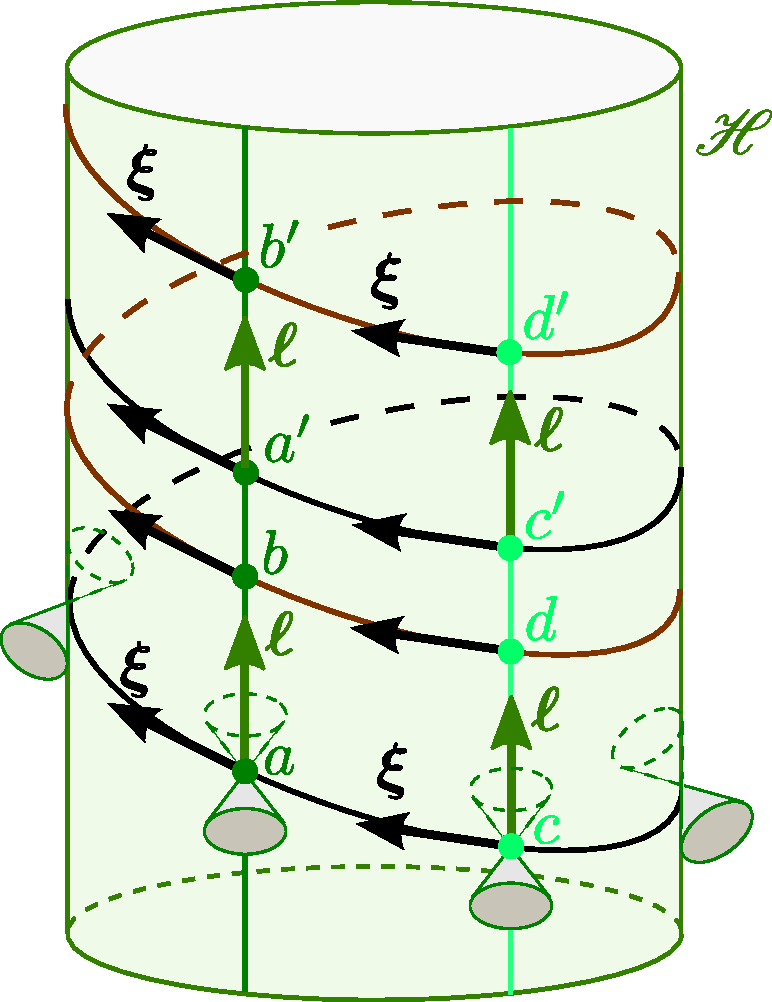
\includegraphics[height=0.4\textheight]{sta_rot_horizon_gen.pdf}
\textbf{\large (a)}
\quad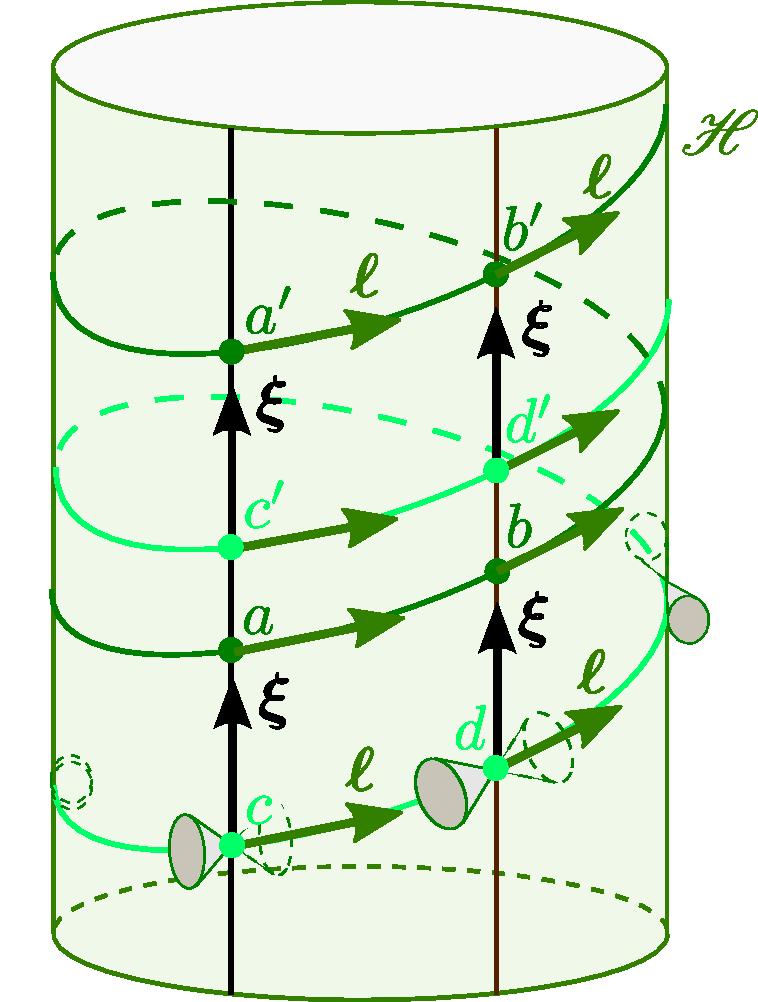
\includegraphics[height=0.4\textheight]{sta_rot_horizon_kil.pdf}
\textbf{\large (b)}}
\caption[]{\label{f:sta:rot_horizon} \footnotesize
Two equivalent representations of an event horizon $\Hor$ with cross-sections of $\SS^n$ topology
and with a stationary Killing vector field $\w{\xi}$ that is
spacelike on $\Hor$:
\textbf{(a)} Representation with the null geodesic generators of $\Hor$ drawn as vertical
lines; two of them are actually depicted, in dark green and light green
respectively, with a null normal $\wl$ along them; besides,
two field lines of $\w{\xi}$
(orbits of the stationary group) are depicted, in black and brown
respectively.
\textbf{(b)} Representation with the field lines of $\w{\xi}$ as vertical lines.
The color code is the same as in (a) and
labelled points ($a$, $b$, etc.) help to identify
the two figures. A few light cones are drawn in each figure; note that $\w{\xi}$,
being spacelike, lies outside of them,
while the null normal $\wl$ is tangent to them.
The strong rigidity theorem (Property~\ref{p:sta:strong_rigidity_thm}) states that
$\wl$ is collinear to a Killing vector field $\w{\chi}$, making $\Hor$
a Killing horizon.}
\end{figure}

When the Killing field $\w{\xi}$ is not null on $\Hor$, we cannot say a priori
that $\Hor$ is a Killing horizon. However, modulo some additional hypotheses,
it turns out that $\Hor$ is still a Killing horizon, albeit with
respect to a Killing vector distinct from $\w{\xi}$. This result is due to
S.W.~Hawking\index[pers]{Hawking, S.W.} (1972)
\cite{Hawki72,HawkiE73} and is known as the
\defin{(strong) rigidity theorem}\index{strong!rigidity theorem}\index{rigidity theorem!strong --}.
We give below a modern version of this theorem, due to
Hollands, Ishibashi \& Wald (2007) \cite{HollaIW07}
and Moncrief \& Isenberg (2008) \cite{MoncrI08} (see also
Theorem~8.1 p.~470 of Choquet-Bruhat's textbook \cite{Choqu09}).

\begin{prop}[strong rigidity theorem]
\label{p:sta:strong_rigidity_thm}
Let $(\M,\w{g})$ be a stationary spacetime of dimension $n\geq 4$ containing a black
hole. Let $\Hor$ be a connected component of the black hole event horizon.
Let us assume that the stationary Killing vector $\w{\xi}$
is spacelike on some parts of $\Hor$. If
\begin{enumerate}
\item $\M$ and $\Hor$ are (real) analytic manifolds
(cf. Remark~\ref{r:bas:analytic} in Sec.~\ref{s:bas:def_manif}),
with $\w{g}$ being an analytic field,
\item $\w{g}$ fulfills the vacuum Einstein equation (\ref{e:fra:vac_Einstein})
or the electrovacuum Einstein equation (\ref{e:fra:electrovac_Einstein}),
\item $n=4$ or $\Hor$ has a null geodesic generator that is incomplete,
\item $\Hor$ has compact cross-sections,
\item $\w{\xi}$ is transverse to some cross-sections,
\end{enumerate}
then the spacetime $(\M,\w{g})$ admits a second Killing vector, $\w{\chi}$
say, such that $\w{\xi}$ and $\w{\chi}$ commute: $[\w{\xi}, \w{\chi}] = 0$ and
$\Hor$ is a Killing horizon with respect to $\w{\chi}$.
\end{prop}

\begin{figure}
\centerline{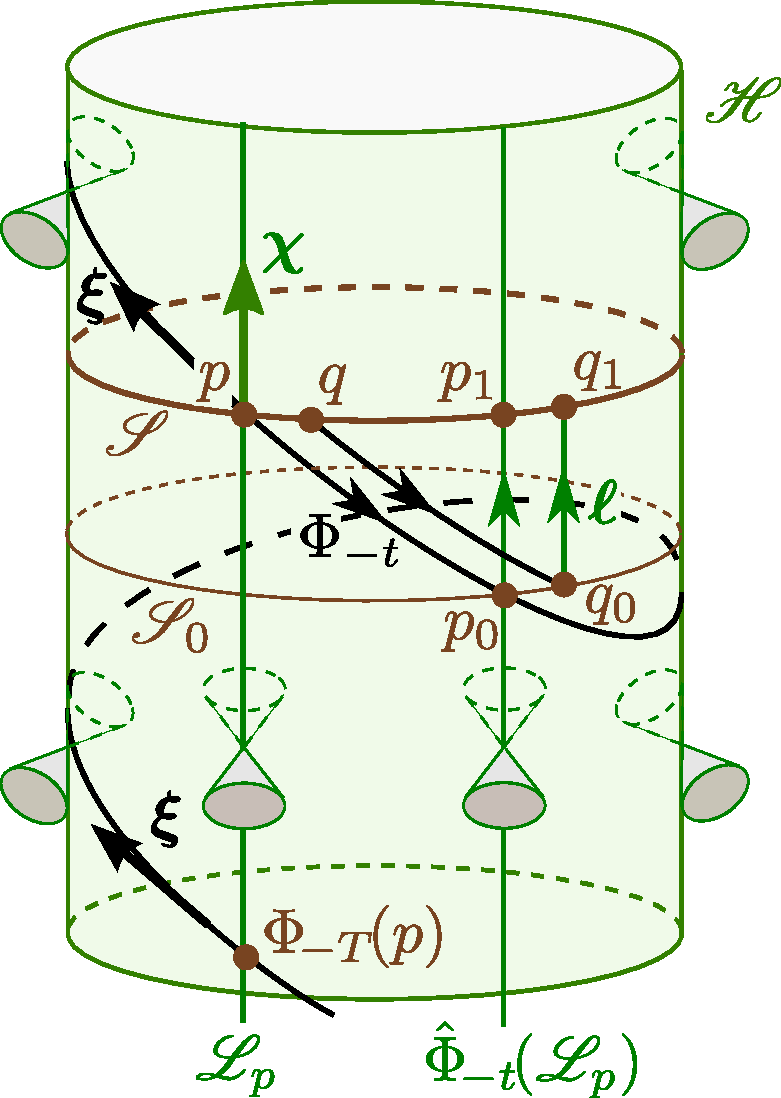
\includegraphics[height=0.4\textheight]{sta_axisym_sections.pdf}}
\caption[]{\label{f:sta:axisym_sections} \footnotesize
Action $\Psi$ induced by the spacetime stationary action $\Phi$ (Killing vector $\w{\xi}$)
on a cross-section $\Sp$ of a rotating event horizon $\Hor$: for $p\in\Sp$ and $t\in\R$,
$\Psi_t(p)$ is denoted by $p_1$ on the figure, while
$p_0 = \Phi_{-t}(p)$. Similarly, for a point $q\in\Sp$
close to $p$, $q_0 = \Phi_{-t}(q)$ and $q_1 = \Psi_t(q)$. Note that this figure is
drawn following the same convention as Fig.~\ref{f:sta:rot_horizon}a, namely the
null geodesic generators of $\Hor$ appear as vertical lines.
}
\end{figure}


\begin{proof}[Sketch of proof]
The proof of the strong rigidity theorem is pretty long and we
give here only a sketch for $n=4$, referring to Hawking \& Ellis' textbook~\cite{HawkiE73} (Proposition~9.3.6)
for full details and to Refs.~\cite{HollaIW07,HollaI12,MoncrI08}
for $n>4$.
Let us thus assume $n=4$ and that the (electro)vacuum Einstein equation holds.
The null dominant energy condition is then satisfied and, since
$\Hor$ is connected, the topology theorem 1 (Property~\ref{p:sta:topology1})
implies that the complete cross-sections of $\Hor$ have the topology of $\SS^2$,
or equivalently that the topology of $\Hor$ is $\R\times\SS^2$.

Let us first show that the
spacetime stationary action $\Phi:\  \R\times \M \to \M$, $(t,p) \mapsto \Phi_t(p)$
induces a $\mathrm{SO}(2)$ action $\hat{\Phi}$ on the set $\mathscr{G}$ of
null geodesic generators of $\Hor$.
Each $\Phi_t$ being an isometry of $(\M,\w{g})$,
it maps any null geodesic $\Li$ of $\Hor$ to a null geodesic $\hat{\Phi}_t(\Li):= \Phi_t(\Li)$.
Morever, since $\Phi_t$ leaves $\Hor$ globally invariant (Property~\ref{p:sta:stationary_hor}),
$\hat{\Phi}_t(\Li)\subset\Hor$, i.e. $\hat{\Phi}_t(\Li)\in\mathscr{G}$.
Let check that $\hat{\Phi}$ obeys the laws of a group action:
obviously $\hat{\Phi}_0(\Li) = \Li$ and for any $(t_1, t_2)\in \R^2$
and $p\in\Li$, we have
$\Phi_{t_2 + t_1}(p)\in\hat{\Phi}_{t_2+t_1}(\Li)$ but
$\Phi_{t_2 + t_1}(p) = \Phi_{t_2}(\Phi_{t_1}(p)) \in \hat{\Phi}_{t_2}(\hat{\Phi}_{t_1}(\Li))$
as well,
from which we conclude that $\hat{\Phi}_{t_2+t_1}(\Li) = \hat{\Phi}_{t_2}(\hat{\Phi}_{t_1}(\Li))$,
given that there is only one null geodesic generator through the point $\Phi_{t_2 + t_1}(p)$.
Since the stationary generator $\w{\xi}$ is assumed to be spacelike on some parts
of $\Hor$, the group action is not trivial: there exist some null generators $\Li$ for which
$\hat{\Phi}_t(\Li)\neq \Li$ (when $\w{\xi}$ is null on a part of $\Hor$, it is necessarily
tangent to a null generator $\Li$, which is then a fixed point of the group action:
$\forall t\in\R, \hat{\Phi}_t(\Li) = \Li$).
Moreover, the group action $\hat{\Phi}$ is periodic: due to the topology
$\R\times\SS^2$ of $\Hor$,
there exists a smallest $T>0$
such that for any null generator $\Li$, $\hat{\Phi}_T(\Li) = \Li$
(cf. Fig.~\ref{f:sta:rot_horizon}, where $a' = \Phi_T(a)$,
$b' = \Phi_T(b)$, $c' = \Phi_T(c)$ and $d' = \Phi_T(d)$, noticing that
each pair $(p,p')$, where $p$ stands for $a$, $b$, $c$ or $d$,
lie on the same null generator). Hence $\hat{\Phi}$ is
a $\mathrm{SO}(2)$ action on the set $\mathscr{G}$
of null generators of $\Hor$, the standard angle parameter $\ph\in[0,2\pi)$ %$]$
of $\mathrm{SO}(2)$ being related to $t\in [0,T)$ by $\ph = 2\pi t / T$. %$]$
Moreover, the $\mathrm{SO}(2)$ action must have exactly two fixed points,
$\Li_1$ and $\Li_2$ say,
for $\mathscr{G}$ has the topology of $\SS^2$: one
can identify $\mathscr{G}$ with an arbitrary complete cross-section $\hat{\Sp}$
of $\Hor$ (each $\Li\in\mathscr{G}$ intersects $\hat{\Sp}$ at a single
point and through each $p\in\hat{\Sp}$ there is a single $\Li\in\mathscr{G}$)
and, as recalled above, all cross-sections have the topology of $\SS^2$.

Let $\Sp$ be a complete cross-section of $\Hor$ such that the stationary Killing
vector $\w{\xi}$ is nowhere tangent to $\Sp$.
Let $\w{q}$ be the metric induced by $\w{g}$ on $\Sp$.
We are going to show that the
spacetime stationary action $\Phi$
induces a $\mathrm{SO}(2)$ action $\Psi: [0,T) \times \Sp \to \Sp$, $(t,p) \mapsto \Psi_t(p)$
such that each $\Psi_t$ is an isometry of $(\Sp,\w{q})$.
For $t\in\R$ and $p\in\Sp$, the point
$\Phi_{-t}(p)$ lies in $\Hor$ since $\Hor$ is globally invariant by
$\Phi_t$ (Property~\ref{p:sta:stationary_hor}). Let then $\Li$ be the unique
null generator of $\Hor$ through $\Phi_{-t}(p)$. Since $\Sp$
is a complete cross-section of $\Hor$, $\Li$ intersects $\Sp$ at a unique
point, which we define as $\Psi_t(p)$ (cf. Fig.~\ref{f:sta:axisym_sections}, where
$\Li$ is denoted $\hat{\Phi}_{-t}(\Li_p)$).
In other words, $\Psi_t(p)$ is obtained by displacing $p$ by a parameter $-t$ along the field lines of $\w{\xi}$ and then going back to $\Sp$ along a null generator of $\Hor$.
Equivalently, we may write
\be \label{e:sta:def_Psi_action}
    \Psi_t(p) = \hat{\Phi}_{-t}(\Li_p)\cap\Sp,
\ee
where $\Li_p$ is the null geodesic generator through $p$ (cf. Fig.~\ref{f:sta:axisym_sections}).
Let us check that $\Psi$ is a 1-parameter group action on $\Sp$,
i.e. fulfills $\Psi_0(p) = p$ and $\Psi_{t_2 + t_1}(p) = \Psi_{t_2} (\Psi_{t_1} (p))$
for any $p\in \Sp$ (cf. Sec.~\ref{s:neh:symmetries}) and $(t_1, t_2)\in \R^2$.
The first property is trivial. Regarding the second one,
$\Psi_{t_1}(p)$ lies on the same
null generator $\Li$ as $\Phi_{-t_1}(p)$ (by definition of $\Psi_{t_1}$).
It follows that both $\Phi_{-t_2}(\Psi_{t_1}(p))$ and
$\Phi_{-t_2}(\Phi_{-t_1}(p))$ lie on the null generator $\hat{\Phi}_{-t_2}(\Li)$.
But $\Phi_{-t_2}(\Phi_{-1}(p)) = \Phi_{-t_2-t_1}(p)$, so that
$\Psi_{t_2 + t_1}(p) = \hat{\Phi}_{-t_2}(\Li) \cap \Sp = \Psi_{t_2} (\Psi_{t_1} (p))$.
Hence $\Psi: \R \times \Sp \to \Sp$, $(t,p) \mapsto \Psi_t(p)$ is 1-parameter
group action on $\Sp$. Moreover this group action inherits the $T$-periodicity
from $\hat{\Phi}$ and thus is a $\mathrm{SO}(2)$ action.
Indeed, Eq.~(\ref{e:sta:def_Psi_action}) implies
$\Psi_T(p) = \hat{\Phi}_{-T}(\Li_p)\cap\Sp = \Li_p \cap \Sp = p$
(see also Fig.~\ref{f:sta:axisym_sections}, where $\Phi_{-T}(p)$ lies on the
same null generator as $p$).

Let us now show that for any $t\in[0,T)$, %$]$
$\Psi_t$ is an isometry of $(\Sp,\w{g})$.
Let $p$ and $q$ be infinitely close points of $\Sp$. Because $\Phi_{-t}$ is
a spacetime isometry, we have
\be \label{e:sta:q_pq_q0_p0q0}
 \w{q}(\vp{pq},\vp{pq}) = \left.\w{g}\right| _p(\vp{pq},\vp{pq})
= \left.\w{g}\right| _{p_0}(\vp{p_0q_0},\vp{p_0q_0}),
\ee
where $p_0 := \Phi_{-t}(p)$ and $q_0 := \Phi_{-t}(q)$ (cf. Fig.~\ref{f:sta:axisym_sections}).
Now, $p_0$ and $q_0$ are two points of $\Sp_0 := \Phi_{-t}(\Sp)$, which
is a complete cross-section of $\Hor$ that has no intersection with $\Sp$ for $t\neq 0$, given that $\w{\xi}$ is transverse to $\Sp$. One can then
choose a parametrization $\lambda$ of the null generators $\Li$ of $\Hor$
such that $\lambda=0$ on $\Sp_0$ and $\lambda=1$ on $\Sp$. Let
$\wl = \left. \D\w{x}/\D\lambda \right| _{\Li}$ be the associated tangent vector.
One may consider that $\Sp_0$ and $\Sp$ are the two ends of a foliation of $\Hor$
by a family $(\Sp_\lambda)_{\lambda\in[0,1]}$ of complete cross-sections
(same construction as in the proof of Property~\ref{p:neh:invariance_area}).
By denoting by $\w{q}$ the metric induced by $\w{g}$ on each of the surfaces
$\Sp_\lambda$, we have $\left.\w{g}\right| _{p_0}(\vp{p_0q_0},\vp{p_0q_0}) = \w{q}(\vp{p_0q_0},\vp{p_0q_0})$. Now, since $\Hor$ is a non-expanding horizon (Property~\ref{p:sta:hor_non_expanding}) and the null
energy condition is fulfilled (since we are considering the (electro)vacuum Einstein equation), the metric $\w{q}$ is preserved along
$\wl$: $\vw{q}^* \Lie{\el} \w{q} = 0$ [Property~\ref{p:neh:invariance_of_2metric}]. Since $p_1:= \Psi_t(p)$ and $q_1:=\Psi_t(q)$
are obtained from $p_0$ and $q_0$ by the same displacement $\delta\lambda=1$
along $\wl$ (cf. Fig.~\ref{f:sta:axisym_sections}),
it follows that $\w{q}(\vp{p_0q_0},\vp{p_0q_0}) =  \w{q}(\vp{p_1 q_1},\vp{p_1 q_1})$.
By combining with Eq.~(\ref{e:sta:q_pq_q0_p0q0}), we get
$\w{q}(\vp{pq},\vp{pq}) = \w{q}(\vp{p_1q_1},\vp{p_1q_1})$, which proves that
$\Psi_t$ is an isometry of $(\Sp, \w{q})$.

At this stage, we have shown that each cross-section of $\Hor$ admits an
isometry group isomorphic to $\mathrm{SO}(2)$, i.e. is axisymmetric.
One thus may say that, in addition to be stationary,
$\Hor$ is axisymmetric, although the concept of axisymmetry as the result of the
metric invariance under a group action (cf. Sec.~\ref{s:neh:symmetries})
is ill-defined for $\Hor$, given that, as a null manifold, $\Hor$
is not endowed with a proper (nondegenerate) metric tensor.

The major step is to show that there exists a Killing vector
field $\w{\chi}$ of $(\M,\w{g})$ that, on $\Hor$, is tangent to the null generators;
it will then follow that the whole spacetime $(\M,\w{g})$ is axisymmetric,
the generator of the $\mathrm{SO}(2)$ isometry being $T/(2\pi)(\w{\chi} - \w{\xi})$.
We first define $\w{\chi}$ on $\Hor$ only, by demanding that $\w{\chi}$ is the tangent vector to the null generators $\Li$ of $\Hor$
corresponding to a parameter $v$ of $\Li$ that is connected to the parameter
$t$ of the stationary action $\Phi$, in the sense that for any point $p$
of a given null generator\footnote{Recall that on $\Hor$, $\Phi_T(p)$ and $p$ always lie on the same null generator.} $\Li$,
\be
\label{e:sta:vPhiT_v_p_T}
    v(\Phi_T(p)) = v(p) + T.
\ee
The above condition is not sufficient to fully specify the parameter $v$, and hence $\w{\chi}$,
along $\Li$. We require in addition that
the non-affinity coefficient $\kappa$ of
$\w{\chi}$ is constant along $\Li$: $\wnab_{\w{\chi}} \kappa = 0$.
In view of Eq.~(\ref{e:def:def_kappa}),
this is equivalent to $\w{\chi} = - \mathrm{e}^{\rho} \, \vw{\nabla} u$
with $\D^2\rho/\D v^2 = 0$ along $\Li$,  where $u$ is a scalar field
such that $\Hor$ is the hypersurface $u=0$.
By construction, the vector field $\w{\chi}$ on $\Hor$ is invariant
under the stationary action, i.e. $\Lie{\xi} \w{\chi} = 0$, so that
$\w{\xi}$ and $\w{\chi}$ commute: $[\w{\xi}, \w{\chi}] = 0$.
Let then define the following vector field on $\Hor$:
\be \label{e:sta:def_eta_rigidity}
    \w{\eta} := \frac{1}{\Omega_{\Hor}} \left( \w{\chi} - \w{\xi} \right) ,
    \qquad \mbox{with}\quad \Omega_{\Hor} := \frac{2\pi}{T} .
\ee
By construction, $\w{\eta}$ has closed field lines of period $2\pi$.
Indeed, since $\w{\xi}$ and $\w{\chi}$ commute, moving by a parameter $2\pi$
along $\w{\eta}$ is equivalent to moving by a parameter $t=-T$ along the field
lines of $\w{\xi}$ and then by a parameter $v=T$ along the field lines of
$\w{\chi}$; the property (\ref{e:sta:vPhiT_v_p_T}) ensures that one is back
to the starting point.
The vector field $\w{\eta}$ vanishes at points where $\w{\xi} = \w{\chi}$,
i.e. at points where $\w{\xi}$ is tangent to some null generator of $\Hor$.
This occurs along null generators that are fixed points of the group
action $\hat{\Phi}$ on $\mathscr{G}$.
As discussed above, there are only two such fixed points, $\Li_1$ and $\Li_2$.
These two null generators
of $\Hor$ define thus the common ``axis'' of all the rotations generated
by $\w{\eta}$.
Let $\mathscr{C}$ be a curve in $\Hor$
from $\Li_1$ and $\Li_2$, orthogonal to $\w{\eta}$ and
such that the field lines of $\w{\eta}$ from $\mathscr{C}$ form
a smooth cross-section $\Sp$ of $\Hor$. Let us then denote by $\Sp_v$ the
cross-section obtained by displacing $\Sp$ by a parameter $v$ along $\w{\chi}$.
Finally, let $\w{k}$ be the future-directed null vector orthogonal to $\Sp_v$ and complementary
to $\w{\chi}$, normalized such that $\w{\chi}\cdot\w{k} = -1$ ($\w{k}$ is
transverse to $\Hor$ and is pointing towards the black hole region).
In a neighborhood of $\Hor$, we introduce a spacetime coordinate system $(v,r,\th,\ph)$,
named \defin{Gaussian null coordinates}\index{Gaussian!null coordinates}, as follows.
First of all, we choose spherical coordinates $(\th,\ph)$ on the cross-section
$\Sp$, such that $\w{\eta} = \wpar_\ph$ and $\th$ is a parameter along
the ``meridional'' curve $\mathscr{C}$. To any point $p\in\Hor$, we assign
then the coordinates $(v,\th,\ph)$ where $v$ is such that $p\in \Sp_v$
and $(\th,\ph)$ are the coordinates
of the intersection of $\Sp$ and the null generator $\Li$ through $p$.
Let us then consider the null geodesics $\Li'$
of tangent vector $\w{k}$, which are transverse to $\Hor$ and an affine parameter
$r$ along each of them such that, on $\Hor$, $r=0$ and $\w{k} = - \D{\w{x}}/\D r$.
To any point $p\in \Li'$ in the vicinity of $\Hor$, we assign the coordinates $(v,r,\th,\ph)$
such that $r$ is the affine parameter of $p$ along $\Li'$ and $(v,\th,\ph)$
are the coordinates of the intersection of $\Li'$ and $\Hor$. We may then extend
the vector fields $\w{\chi}$, $\w{\eta}$ and $\w{k}$ away from $\Hor$ by setting
\[
    \w{\chi} := \wpar_v,\quad
    \w{\eta} := \wpar_\ph,\quad
    \w{k} := - \wpar_r .
\]
By means of the (electro)vacuum Einstein equation, one can then show by induction that,
\be \label{e:sta:Lie_k_Lie_chi_g}
    \forall N\in\mathbb{N}, \quad \underbrace{\Lie{k}\cdots \Lie{k}}_{N\mbox{\ times}}
    \Lie{\chi} \w{g} \equalH 0 .
\ee
This is the lengthy part of the computation (see p.~343 of Ref.~\cite{HawkiE73}).
Once (\ref{e:sta:Lie_k_Lie_chi_g})
is established, one can use the analyticity hypothesis to conclude that $\Lie{\chi} \w{g} = 0$
in all $\M$, i.e. that $\w{\chi}$ is a Killing vector of $(\M,\w{g})$. Since, on $\Hor$,
$\w{\chi}$ is normal to $\Hor$, it follows that $\Hor$ is a Killing horizon
with respect to $\w{\chi}$.
\end{proof}

\begin{remark}
For $n\neq 4$, the Killing horizon $\Hor$ is necessarily non-degenerate, given
that $\Hor$ must have an incomplete null geodesic generator in that case
(third hypothesis of the theorem).
\end{remark}

\begin{remark}
For $n=4$, the stationary Killing vector $\w{\xi}$ cannot be spacelike
on the whole of $\Hor$: it is indeed null on the rotation axis, i.e.
at the points where $\w{\eta} = 0$, given that Eq.~(\ref{e:sta:def_eta_rigidity})
implies $\w{\xi} = \w{\chi}$ for $\w{\eta}=0$.
\end{remark}

\begin{remark}
In some formulations \cite{HollaIW07,HawkiE73}, the hypothesis of $\w{\xi}$
being transverse to some cross-sections is replaced by $\Hor$ lying in
the future of the past infinity $\scri^-$. Actually it can be shown
that the latter implies the former (see e.g. the proof of Proposition~9.3.1
in Ref.~\cite{HawkiE73}).
\end{remark}

\begin{remark} \label{r:sta:non_Killing}
The strong ridigity theorem may not hold in theories of gravity distinct
from general relativity (hypothesis~2 of Property~\ref{p:sta:strong_rigidity_thm}).
For instance, the so-called \emph{disformed Kerr solution}\index{disformed Kerr solution}\index{Kerr!metric!disformed --}
\cite{AnsonBCH21,BenAc_al20}
describes a $n=4$ stationary black hole in a higher-order scalar-tensor theory (belonging to the
so-called \emph{DHOST}\index{DHOST} family, for \emph{Degenerate Higher-Order Scalar-Tensor} \cite{Langl19}), the event horizon of which does not seem to be a Killing horizon
\cite{AnsonBCH21}.
\end{remark}


\begin{hist}
Stephen Hawking\index[pers]{Hawking, S.W.} first established the strong rigidity
theorem in 1972 \cite{Hawki72}
for a spacetime of dimension $n=4$ and assuming that there exists
a past event horizon (i.e. a white hole region) in addition to the
future event horizon $\Hor$.
The theorem was restated and proved without the white hole hypothesis
in Hawking \& Ellis'\index[pers]{Ellis, G.F.R.} famous textbook published in 1973 \cite{HawkiE73}
(Proposition 9.3.6).
An account by Hawking himself
about this reformulation can be found in
Sec.~8 of Ref.~\cite{Hawki73}. The demonstration presented in Ref.~\cite{HawkiE73}
relies on the vacuum Einstein equation,
but it is noted there that \emph{``similar arguments hold in the presence
of matter fields, like the electromagnetic or scalar fields, which obey
well-behaved hyperbolic equations''}.
Some details in Hawking's proof have been fixed
by Piotr T. Chru\'sciel\index[pers]{Chrusciel, P.T.@Chru\'sciel, P.T.} in 1997 \cite{Chrus97}.
The extension to spacetimes of
dimension $n\geq 4$ has been performed independently by
Stefan Hollands\index[pers]{Hollands, S.}, Akihiro Ishibashi\index[pers]{Ishibashi, A.}
and Robert M.~Wald\index[pers]{Wald, R.M.} in 2007 \cite{HollaIW07}
and by Vincent Moncrief\index[pers]{Moncrief, V.} and James Isenberg\index[pers]{Isenberg, J.}
in 2008 \cite{MoncrI08}. The treatment of the electrovacuum
case is done explicitly in Hollands, Ishibashi \& Wald's work \cite{HollaIW07}.
\end{hist}

The strong rigidity theorem relies on the rather strong assumption that
the manifolds and fields are analytic.
On physical grounds,
it would be desirable to assume only \emph{smooth} manifolds and fields.
In 1999, H. Friedrich\index[pers]{Friedrich, H.}, I. Rácz\index[pers]{Racz, I.@R\'acz, I.},
and R.M. Wald\index[pers]{Wald, R.M.} \cite{FriedRW99} could remove the analyticity hypothesis but only
towards the \emph{interior} of the black hole, i.e. they could prove that
the vector $\w{\chi}$ normal to $\Hor$ can be extended to a Killing vector
of the black hole interior.
Another partial success has been achieved in 2014 by
S.~Alexakis\index[pers]{Alexakis, S.}, A.D.~Ionescu\index[pers]{Ionescu, A.D.} and
S.~Klainerman\index[pers]{Klainerman, S.} \cite{AlexaIK14}, who proved
the strong rigidity theorem without the analyticity
assumption, but only for slowly rotating black holes.
See Ref.~\cite{IonesK15} for a review of the progresses in removing
the analyticity hypothesis.

It turns out that, for each connected component of the even horizon, the
Killing vector $\w{\chi}$ is expressible as a linear combination of
the stationary Killing vector $\w{\xi}$ and some Killing vectors
generating axisymmetries:

\begin{prop}[axisymmetry\index{axisymmetric spacetime} of stationary black holes]
\label{p:sta:axisymmetry_BH}
Under the same hypotheses as in Property~\ref{p:sta:strong_rigidity_thm},
there exist $L$ Killing vectors $\w{\eta}_{(1)},\ldots,\w{\eta}_{(L)}$
with $1 \leq L \leq [(n-1)/2]$, which have closed orbits of period $2\pi$,
such that
\be
   [\w{\xi},\w{\eta}_{(i)}] = 0 \qand [\w{\eta}_{(i)},\w{\eta}_{(j)}] = 0
   \quad (1 \leq i, j \leq L)
\ee
and the Killing vector $\w{\chi}$ normal to $\Hor$ writes
\be \label{e:sta:chi_xi_Omega_i_eta_i}
    \w{\chi} = \w{\xi} + \Omega^{(1)} \w{\eta}_{(1)} + \cdots \Omega^{(L)} \w{\eta}_{(L)} ,
\ee
where $\Omega^{(1)}$, $\ldots$, $\Omega^{(L)}$ are $L$ constants, all of whose
ratios are irrational.

For $n=4$, one has $[(n-1)/2] = 1$, so that necessarily $L=1$. Denoting
$\w{\eta}_{(1)}$ simply by $\w{\eta}$ and $\Omega^{(1)}$ by $\Omega_{\Hor}$,
Eq.~(\ref{e:sta:chi_xi_Omega_i_eta_i}) reduces to
\be \label{e:sta:chi_xi_OmegaH_eta}
    \w{\chi} = \w{\xi} + \Omega_{\Hor} \w{\eta} .
\ee
The constant $\Omega_{\Hor}$ is then called the
\defin{black hole rotation velocity}\index{black!hole!rotation velocity}\index{rotation!velocity} if $\Hor$ coincides with
the whole event horizon (i.e. if the event horizon is connected).
\end{prop}

Since it has closed orbits, the isometry group generated by each Killing vector
$\w{\eta}_{(i)}$ is $\mathrm{SO}(2)$. Each isometry is thus an
axisymmetry,
according to the definition given in Sec.~\ref{s:sta:Komar_angu_mom}.
For $n=4$, Eq.~(\ref{e:sta:chi_xi_OmegaH_eta}) is
equivalent to Eq.~(\ref{e:sta:def_eta_rigidity}).
The constancy of $\Omega_{\Hor}$ in Eq.~(\ref{e:sta:chi_xi_OmegaH_eta})
can be interpreted by saying that the event horizon is rotating rigidly
(no differential rotation) and justifies the name \emph{rigidity theorem}.
For $n>4$, we refer
to the original articles \cite{HollaIW07,MoncrI08} for the proof
of Property~\ref{p:sta:axisymmetry_BH}.

\begin{remark}
Property~\ref{p:sta:axisymmetry_BH} is often considered as the second part
of the strong rigidity theorem. In some statements, it is even incorporated
into the strong rigidity theorem (e.g. Proposition~9.3.6 of Ref.~\cite{HawkiE73}).
\end{remark}

\begin{remark}
\label{r:sta:dep_eta_Omega}
If the event horizon has various connected components, the Killing vectors
$\w{\eta}_{(i)}$ and the constants $\Omega^{(i)}$ may vary from one connected
component to the other. In particular, the horizon-generating Killing vector $\w{\chi}$
may not be the same for each connected component. For instance,
in dimension $n=5$, the \emph{black saturn}\index{black!saturn}
found by H.~Elvang\index[pers]{Elvang, H.} and P.~Figueras\index[pers]{Figureas, P.} in 2007 \cite{ElvanF07}
is a stationary black hole, the event horizon of which has two connected
components: $\Hor_{\rm p}$ (the ``planet'') and $\Hor_{\rm r}$ (the ``ring''),
with topology $\R\times\SS^3$ and $\R\times\SS^1\times\SS^2$ respectively.
For both $\Hor_{\rm p}$ and $\Hor_{\rm r}$, $L=1$ and
the two components share the same axisymmetry Killing vector $\w{\eta}_{(1)}$,
but they may have different angular velocities:
$\Omega^{(1)}_{\Hor_{\rm p}} \neq \Omega^{(1)}_{\Hor_{\rm r}}$, and hence
different normal Killing vectors: $\w{\chi}_{\Hor_{\rm p}} \neq \w{\chi}_{\Hor_{\rm r}}$.
\end{remark}

In the literature, the strong rigidity theorem is sometimes called
simply the \emph{rigidity theorem}\index{rigidity theorem}, without the qualifier \emph{strong}
(e.g. Refs.~\cite{Choqu09,HollaI12}).
The terminology \emph{strong rigidity}, employed in Refs.~\cite{Carte99,ChrusLH12,Heusl96},
aims to distinguish from the so-called
\emph{weak rigidity theorem}\index{weak!rigidity theorem}\index{rigidity theorem!weak --}
proved by Carter in 1969 (corollary to Theorem~1 in Ref.~\cite{Carte69}; see also \cite{Carte72}, Sec.~4.5 of Ref.~\cite{Carte87} and Sec.~6.3 of Ref.~\cite{Heusl96}). The latter asserts that the event horizon of a black hole in a stationary, axisymmetric
and circular\footnote{A stationary and axisymmetric spacetime is said to be \defin{circular}\index{circular!spacetime} iff the $\R\times\mathrm{SO}(2)$ group action
is \defin{orthogonally transitive}\index{orthogonally transitive}, i.e. the 2-surfaces generated by the two commuting
Killing vectors $\w{\xi}$ and $\w{\eta}$ are orthogonal to a family of $(n-2)$-dimensional surfaces \cite{Carte69}.}
spacetime must be a Killing horizon. The \emph{strong rigidity theorem} is
stronger in that it assumes only the stationarity of the spacetime, the axisymmetry
becoming a consequence (Property~\ref{p:sta:axisymmetry_BH}). On the other hand,
the weak rigidity theorem is stronger in so far as it does not rely on
the Einstein equation, nor on the assumption of analyticity.

By the very definition of stationarity, the Killing vector field $\w{\xi}$ is
timelike in the vicinity of $\scri^+$ and $\scri^-$. If $\w{\xi}$ is spacelike
on some parts of $\Hor$, as assumed in this section, by continuity it must be spacelike
in some part of the domain of outer communications $\langle\langle \M\rangle\rangle$
near $\Hor$. The simplest configuration is when
$\w{\xi}$ is spacelike in some connected region $\mathscr{G}\subset \langle\langle \M\rangle\rangle$
around $\Hor$, null at the boundary of $\mathscr{G}$ and timelike outside $\mathscr{G}$
up to $\scri^+$ and $\scri^-$. The subset $\mathscr{G}$ is
called the \defin{ergoregion}\index{ergoregion} and its boundary $\E:=\partial\mathscr{G}$
the \defin{ergosphere}. We shall discuss it further in Chap.~\ref{s:ker},
especially in connection with the so-called \emph{Penrose process}
(Sec.~\ref{s:gek:Penrose_proc}).

\subsection{Extremal black holes} \label{s:sta:extremal_BH}

Properties~\ref{p:sta:H_Killing_hor_xi_null} and \ref{p:sta:strong_rigidity_thm},
show that, under some rather generic hypotheses (at least as far as general
relativity is concerned, cf. Remark~\ref{r:sta:non_Killing}),
the event horizon of a stationary black hole, if connected,
is a Killing horizon. Now, in Sec.~\ref{s:neh:classif_KH}
we have classified Killing horizons in two
categories: the degenerate ones
(zero surface gravity) and the non-degenerate ones
(nonzero surface gravity). This justifies the
following definition:

\begin{greybox}
A black hole in a stationary spacetime is said to be \defin{extremal}\index{extremal!black hole} (resp. \defin{non-extremal}\index{non-extremal black hole}) if, and
only if, its event horizon $\Hor$ is a degenerate (resp. non-degenerate) Killing horizon.
\end{greybox}

The surface gravity $\kappa$ of an extremal black hole is identically zero and
the null generators of its horizon are \emph{complete} geodesics: the parameter $t$
associated to the stationary Killing $\w{\xi}$ is an affine parameter ranging
in the whole of $\R$.
Standard examples are the extremal Reissner-Norström black hole (presented
briefly in Sec.~\ref{s:sta:uniqueness_static}) and
the extremal Kerr black hole (to be discussed in Chap.~\ref{s:exk}).


%%%%%%%%%%%%%%%%%%%%%%%%%%%%%%%%%%%%%%%%%%%%%%%%%%%%%%%%%%%%%%%%%%%%%%%%%%%%%%%

\section{The generalized Smarr formula} \label{s:sta:Smarr}

As shown in the previous section, under some hypotheses, the connected components of the event horizon of a stationary black hole are Killing horizons; this gives rise to a nice formula connecting the
mass, angular momentum and area of these objects. After having established
the formula in the most general case (Sec.~\ref{s:sta:Smarr_general}),
we shall specialize it to electrovacuum black holes (Sec.~\ref{s:sta:Smarr_electrovac}).

\subsection{General form} \label{s:sta:Smarr_general}

\begin{prop}[generalized Smarr formula]
\label{p:sta:Smarr_gen}
Let $(\M,\w{g})$ be a stationary spacetime of dimension $n \geq 4$ (stationary
Killing vector $\w{\xi}$) that contains a black
hole, the event horizon of which has $K \geq 1$ connected components
$\Hor_{1}$, $\ldots$, $\Hor_{K}$.
We shall assume that each $\Hor_{k}$ is a Killing horizon
with respect to a Killing vector $\w{\chi}_{k}$.
This is guaranteed with $\w{\chi}_k = \w{\xi}$
if $\Hor_{k}$ is non-rotating ($\w{\xi}$ null on all $\Hor_{k}$;
Property~\ref{p:sta:H_Killing_hor_xi_null}), while if
$\Hor_{k}$ is rotating ($\w{\xi}$ spacelike on some parts of $\Hor_{k}$),
this holds under the hypotheses of the strong rigidity theorem
(Property~\ref{p:sta:strong_rigidity_thm}),
with $\w{\chi}_{k} = \w{\xi} + \sum_{i=1}^{L_{k}} \Omega^{(i)}_{\Hor_k} \w{\eta}_{\Hor_k(i)}$,
where the $\Omega^{(i)}_{\Hor_k}$ are constants and
the $\w{\eta}_{\Hor_k(i)}$ are axisymmetric Killing vectors
(Property~\ref{p:sta:axisymmetry_BH}).
Being a non-expanding horizon, each
$\Hor_{k}$ has a well defined area $A_{k}$ (Property~\ref{p:neh:invariance_area}).
Let $\kappa_{k}$ be the surface gravity of $\Hor_{k}$, i.e.
the coefficient such that
$\wnab_{\w{\chi}_{k}}\w{\chi}_{k} =  \kappa_{k} \w{\chi}_{k}$
 on $\Hor_{k}$ [cf. Eq.~(\ref{e:neh:xi_nab_xi_kappa})].
Let us assume that the null dominance condition (\ref{e:neh:null_dominant_cond}) is fulfilled
on $\Hor_{k}$ or that $\Hor_{k}$ is part of a bifurcate Killing horizon;
by the zeroth law of black hole dynamics (Property~\ref{p:neh:zeroth_law} or Property~\ref{p:neh:zeroth_law_bifur}), this implies that $\kappa_{k}$ is constant.
Then the Komar mass $M_{\Hor_{k}}$ over any cross-section
of $\Hor_{k}$, as defined by Eq.~(\ref{e:sta:def_Komar_mass}), obeys
\be \label{e:sta:Smarr_H_k}
    M_{\Hor_{k}} = \frac{n - 2}{2(n- 3)}\left(
    \frac{\kappa_{k} A_{k}}{4\pi}
    + 2  \sum_{i=1}^{L_{k}} \Omega^{(i)}_{\Hor_k} J_{\Hor_{k}}^{(i)} \right) ,
\ee
where $J_{\Hor_{k}}^{(i)}$ is the Komar angular momentum with respect to
the axisymmetric Killing vector $\w{\eta}_{\Hor_k(i)}$ over
any cross-section of $\Hor_{k}$
as given by Eq.~(\ref{e:sta:def_Komar_J}).
In Eq.~(\ref{e:sta:Smarr_H_k}), it is intended that $L_{k} = 0$ if
$\w{\chi}_{k} = \w{\xi}$, so that there is no sum over $i$ in that case.
Furthermore, the Komar mass at infinity
(cf. Property~\ref{p:sta:Komar_mass_inf}) obeys the \defin{generalized Smarr formula}\index{generalized!Smarr formula}\index{Smarr formula!generalized --}:
\be
\label{e:sta:Smarr_M_infty_R}
    \encadre{ \frac{2(n- 3)}{n - 2}  M_\infty = \sum_{k = 1}^K
    \left(
    \frac{\kappa_{k} A_{k}}{4\pi}
    + 2  \sum_{i=1}^{L_{k}} \Omega^{(i)}_{\Hor_k} J_{\Hor_{k}}^{(i)} \right)
     + \frac{1}{4\pi}  \int_{\Sigma} \w{R}(\w{\xi}, \w{n}) \sqrt{\gamma} \, \D^{n-1} x },
\ee
where $\Sigma$ is any asymptotically flat spacelike hypersurface, the inner boundary
of which is a cross-section of the event horizon, i.e. some union of cross-sections
of the connected components $\Hor_{k}$,
$\w{R}$ is the Ricci tensor of $\w{g}$
and $\w{n}$ is the future-directed unit normal
to $\Sigma$.
If $\w{g}$ obeys the Einstein equation (\ref{e:fra:Einstein_eq_n})
with $\Lambda=0$, this formula can be rewritten as
\bea
    \frac{2(n- 3)}{n - 2}  M_\infty & = & \sum_{k = 1}^K
    \left(
    \frac{\kappa_{k} A_{k}}{4\pi}
    + 2  \sum_{i=1}^{L_{k}} \Omega^{(i)}_{\Hor_k} J_{\Hor_{k}}^{(i)} \right) \nonumber \\
    & & + 2
    \int_{\Sigma} \left( \w{T}(\w{\xi}, \w{n}) - \frac{T \w{\xi}\cdot \w{n}}{n-2}  \right)
    \sqrt{\gamma} \, \D^{n-1} x , \label{e:sta:Smarr_M_infty}
\eea
where $\w{T}$ is the matter energy-momentum tensor.
\end{prop}

\begin{proof}
Let us evaluate the Komar mass $M_{\Hor_k}$ via
formula~(\ref{e:sta:Komar_mass_flux_nabla_xi}).
If we denote the cross-section of $\Hor_{k}$
by $\Sp_{k}$ and we substitute $\w{\xi}$ by
its expression arising from Eq.~(\ref{e:sta:chi_xi_Omega_i_eta_i}), we
get\footnote{Here we drop the index ${k}$ on $\w{\chi}$ and the label $\Hor_k$
on $\Omega^{(i)}$ and $\w{\eta}_{(i)}$ for clarity, given that the integral regards
a single connected component $\Hor_k$.}
\bea
    M_{\Hor_{k}} &= & - \frac{n-2}{16\pi(n-3)} \int_{\Sp_{k}} \nabla_\mu
    \left( \chi_{\nu} - \sum_{i=1}^{L_{k}} \Omega^{(i)}  \eta_{(i)\nu}
    \right) \D S^{\mu\nu} \nonumber \\
    & = & - \frac{n-2}{16\pi(n-3)} \Bigg[
        \underbrace{\int_{\Sp_{k}} \nabla_\mu \chi_\nu \, \D S^{\mu\nu}}_{-2 \kappa_{k} A_{k}}
        - \sum_{i=1}^{L_{k}} \Omega^{(i)}
        \underbrace{\int_{\Sp_{k}} \nabla_\mu \eta_{(i)\nu}
        \, \D S^{\mu\nu}}_{16\pi J_{\Hor_{k}}^{(i)}} \Bigg] . \nonumber
\eea
The second surface integral being $16\pi J_{\Hor_{k}}^{(i)}$ follows
directly from Eq.~(\ref{e:sta:J_Komar_cov_der}).
As for the first integral, the value $-2 \kappa_{k} A_{k}$
is obtained by introducing a null vector $\w{k}$ normal to $\Sp_{k}$
such that $\w{\chi}\cdot\w{k} = -1$.
At each point $p\in\Sp_{k}$,
the pair $(\w{\chi},\w{k})$ is then a null basis of the 2-plane $T_p^\perp\Sp_{k}$
(cf. Fig.~\ref{f:def:TS_ortho} where $\wl$ stands for $\w{\chi}$) and
we may rewrite the area element normal bivector $\D S^{\alpha\beta}$
as\footnote{This follows readily by setting $\w{n} = (\w{\chi} + \w{k})/\sqrt{2}$
and $\w{s} = (\w{\chi} - \w{k})/\sqrt{2}$ in formula~(\ref{e:sta:area_bivector}).}
\be \label{e:sta:dS_chi_k}
    \D S^{\alpha\beta} = (\chi^\alpha k^\beta - k^\alpha \chi^\beta) \sqrt{q}\, \D^{n-2} x .
\ee
We have then
\bea
 \nabla_\mu \chi_\nu \, \D S^{\mu\nu} & = & \Big( \chi^\mu \nabla_\mu \chi_\nu \,  k^\nu
 - k^\mu \chi^\nu \underbrace{\nabla_\mu \chi_\nu}_{-\nabla_\nu \chi_\mu} \Big) \sqrt{q}\, \D^{n-2} x =  2 \underbrace{\chi^\mu \nabla_\mu \chi_\nu}_{\kappa_{k} \chi_\nu} \,  k^\nu \, \sqrt{q}\, \D^{n-2} x \nonumber \\
 & = & 2 \kappa_{k} \underbrace{\chi_\nu k^\nu}_{-1} \, \sqrt{q}\, \D^{n-2} x
    = - 2 \kappa_{k} \, \sqrt{q}\, \D^{n-2} x . \nonumber
\eea
Given that $\kappa_{k}$ is constant (Property~\ref{p:neh:zeroth_law} or Property~\ref{p:neh:zeroth_law_bifur}),
the integral
of the above expression over $\Sp_{k}$ reduces to $-2\kappa_{k} A_{k}$, by the
very definition of the area $A_{k}$ [cf. Eq.~(\ref{e:neh:total_area})].
This establishes Eq.~(\ref{e:sta:Smarr_H_k}).
Finally, Eq.~(\ref{e:sta:Smarr_M_infty_R}) follows from
Eqs.~(\ref{e:sta:def_M_infty}), (\ref{e:sta:Komar_mass_vol_integ_R}) and (\ref{e:sta:Smarr_H_k}), once
one has noticed that $\Sp_{\rm int} = \bigcup_{k=1}^K \Sp_{k}$,
so that $M_{\Sp_{\rm int}} = \sum_{k=1}^K M_{\Hor_{k}}$.
\end{proof}

For vacuum black holes of general relativity, $\w{T} = 0$, the null dominance condition is trivially fulfilled and the generalized Smarr formula (\ref{e:sta:Smarr_M_infty})
simplifies since the integral
term disappears.


\begin{example}[black saturn]
For the \emph{black saturn}\index{black!saturn} solution discussed in Remark~\ref{r:sta:dep_eta_Omega},
one has $n=5$, $K=2$, $L_1 = L_2 = 1$ and formula (\ref{e:sta:Smarr_H_k})
reduces to
\be \label{e:sta:Smarr_H_k_saturn}
    M_{\Hor_{k}} = \frac{3}{32\pi} \kappa_{k} A_{k}
    + \frac{3}{2} \Omega_{\Hor_k} J_{\Hor_k}, \qquad k \in \{1, 2\} ,
\ee
where $k=1$ corresponds to the ``planet'' component of the event horizon
and $k=2$ corresponds to the ``ring'' component. Equation~(\ref{e:sta:Smarr_H_k_saturn})
coincides with the two formulas given in Eq.~(3.43) of the discovery
article \cite{ElvanF07}, which were obtained from the explicit expressions of $M_{\Hor_{k}}$,
$A_k$, $J_{\Hor_k}$, $\kappa_k$ and $\Omega_{\Hor_k}$ in terms of the solution parameters.
For the same solution, the Smarr formula (\ref{e:sta:Smarr_M_infty}) with $\w{T}=0$ is recovered
by combining Eqs.~(3.36) and (3.43) of Ref.~\cite{ElvanF07}.
\end{example}

It is worth to specialize the generalized Smarr formula to
a 4-dimensional spacetime and to a connected event horizon,
by setting $n=4$, $K=1$ and $L_{1}=1$ (cf. Property~\ref{p:sta:axisymmetry_BH})
in Eqs.~(\ref{e:sta:Smarr_H_k}), (\ref{e:sta:Smarr_M_infty_R}) and (\ref{e:sta:Smarr_M_infty}):

\begin{prop}[4-dimensional generalized Smarr formula]
\label{p:sta:Smarr_n4}
Let $(\M, \w{g})$ be a 4-dimensional stationary spacetime
(stationary Killing vector $\w{\xi}$) containing
a black hole with a connected event horizon $\Hor$.
If $\Hor$ is non-rotating ($\w{\xi}$ null on all $\Hor$), it is necessarily
a Killing horizon with respect to $\w{\xi}$. If $\Hor$ is rotating
($\w{\xi}$ partly spacelike on $\Hor$), we shall assumes that
the hypotheses of the strong rigidity theorem
(Property~\ref{p:sta:strong_rigidity_thm}) are fulfilled, so that
$\Hor$ is a Killing horizon with respect to the
Killing vector $\w{\chi} = \w{\xi} + \Omega_{\Hor} \w{\eta}$
[Eq.~(\ref{e:sta:chi_xi_OmegaH_eta})],
where $\Omega_{\Hor}$ is the angular velocity of $\Hor$ and $\w{\eta}$ is
an axisymmetric Killing vector.
We shall combine these two cases by stating
that the former corresponds to $\Omega_{\Hor} = 0$, so that $\w{\chi} = \w{\xi}$.
The surface gravity $\kappa$ of $\Hor$ is defined by the identity
$\wnab_{\w{\chi}}\w{\chi} \equalH \kappa \w{\chi}$ [cf. Eq.~(\ref{e:neh:xi_nab_xi_kappa})].
Assuming that the null dominance condition (\ref{e:neh:null_dominant_cond}) is fulfilled
on $\Hor$ or that $\Hor$ is part of a bifurcate Killing horizon,
the zeroth law of black hole dynamics (Property~\ref{p:neh:zeroth_law} or \ref{p:neh:zeroth_law_bifur})
leads to $\kappa = \mathrm{const}$.
Then the Komar mass $M_{\Hor}$ over any cross-section
of $\Hor$ [cf. Eq.~(\ref{e:sta:def_Komar_mass})] obeys
\be
    M_{\Hor} = \frac{\kappa}{4\pi} A + 2 \Omega_{\Hor} J_{\Hor} ,
\ee
where $A$ is the area of $\Hor$ (cf. Property~\ref{p:neh:invariance_area})
and $J_{\Hor}$ is the Komar angular momentum over any cross-section
of $\Hor$ [cf. Eq.~(\ref{e:sta:def_Komar_J})].
Furthermore, the Komar mass at infinity
(cf. Property~\ref{p:sta:Komar_mass_inf}) obeys\index{Smarr formula!4-dimensional --}
\be \label{e:sta:Smarr_M_infty_n4_R}
   \encadre{ M_\infty = \frac{\kappa}{4\pi} A + 2 \Omega_{\Hor} J_{\Hor}
    +  \frac{1}{4\pi}  \int_{\Sigma} \w{R}(\w{\xi}, \w{n}) \sqrt{\gamma} \, \D^3 x },
\ee
where $\Sigma$ is an asymptotically flat spacelike hypersurface, the inner boundary
of which is a cross-section of $\Hor$,
$\w{R}$ is the Ricci tensor of $\w{g}$ and
$\w{n}$ is the future-directed unit normal to $\Sigma$.
If $\w{g}$ obeys the Einstein equation (\ref{e:fra:Einstein_eq_n})
with $\Lambda=0$, this formula can be rewritten as
\be \label{e:sta:Smarr_M_infty_n4}
    M_\infty = \frac{\kappa}{4\pi} A + 2 \Omega_{\Hor} J_{\Hor}
    + \int_{\Sigma} \left(2 \w{T}(\w{\xi}, \w{n}) - T\,  \w{\xi}\cdot \w{n}  \right)
    \sqrt{\gamma} \, \D^3 x ,
\ee
where $\w{T}$ is the matter energy-momentum tensor.
\end{prop}


\begin{example}[Schwarzschild black hole]
The Schwarzschild black hole will be discussed in details in Chap.~\ref{s:sch};
however, we have sufficiently studied its event horizon in various examples
of the preceding chapters to check that the Smarr formula holds
for it. From Example~\ref{x:def:Schw_hor3} of Chap.~\ref{s:def}, we have
$\kappa = 1/(4 m)$ [Eq.~(\ref{e:def:kappa_Schw_hor})], while from
Example~\ref{x:neh:Schwarz_hor_area} of Chap.~\ref{s:neh} we have
$A = 16\pi m^2$ [Eq.~(\ref{e:neh:area_Schwarz})]. Hence
$\kappa A / (4\pi) = m$. Since we have seen in Example~\ref{x:sta:Komar_mass_infty_Schwarz}
of the current chapter that the parameter $m$ is nothing but the Komar mass
at infinity $M_\infty$, we get
\be
    M_\infty = \frac{\kappa}{4\pi} A .
\ee
This is nothing but the Smarr formula (\ref{e:sta:Smarr_M_infty_n4})
for a static ($\Omega_{\Hor} = 0$) black hole in vaccum ($\w{T}=0$).
\end{example}

\subsection{Smarr formula for charged black holes} \label{s:sta:Smarr_electrovac}

Beside the vacuum case, the generalized Smarr formulas (\ref{e:sta:Smarr_M_infty})
and (\ref{e:sta:Smarr_M_infty_n4}) simplifies significantly for
electrovacuum spacetimes, i.e. spacetimes ruled by general relativity and
for which $\w{T}$ is the energy-momentum
tensor of a source-free electromagnetic field (cf. Sec.~\ref{e:fra:electrovacuum}).
To perform the computation of the integral involving $\w{T}$,
we need first to characterize a stationary electromagnetic field on
a Killing horizon:

\begin{prop}[electromagnetic field on a Killing horizon]
\label{p:sta:electromag_Killing_hor}
Let $(\M,\w{g})$ be a $n$-dimensional asymptotically flat spacetime endowed with some Killing vector field $\w{\chi}$
and containing a Killing horizon $\Hor$ with respect to $\w{\chi}$.
Let us assume
that $(\M,\w{g})$ is endowed with an electromagnetic field $\w{F}$ that respects the
symmetry generated by $\w{\chi}$,
i.e. that obeys $\Lie{\chi} \w{F} = 0$. Furthermore let us
assume that the electrovacuum Einstein equation is fulfilled by $(\w{g},\w{F})$
(cf. Sec.~\ref{e:fra:electrovacuum}). Then the pseudo-electric field\footnote{If $\w{\chi}$
were a unit timelike vector, $\w{E}$ would be a genuine electric field\index{electric!field}:
the one measured by the observer of 4-velocity $\w{\chi}$.}
$\w{E}$ defined by
\be \label{e:sta:def_elec_field}
    \w{E} := \w{F}(., \w{\chi}) \iff E_\alpha := F_{\alpha\mu} \chi^\mu
\ee
is an exact 1-form:
\be \label{e:sta:E_d_Phi}
    \w{E} = - \dd \Phi ,
\ee
where the scalar potential $\Phi$ is expressible in terms of any electromagnetic
potential $\w{A}$ that obeys the $\w{\chi}$-symmetry (i.e. any 1-form $\w{A}$ such that $\w{F} = \dd \w{A}$ and $\Lie{\chi}\w{A} = 0$) by
\be \label{e:sta:Phi_A_chi}
    \Phi = - \langle \w{A}, \w{\chi} \rangle + \mathrm{const}
    \iff
    \Phi =  - A_\mu \chi^\mu + \mathrm{const} .
\ee
We shall choose the additive constant so that $\Phi \to 0$ in the asymptotic flat end
of $(\M,\w{g})$. This determines $\Phi$ uniquely and we shall call it the
\defin{Killing electric potential associated to} $\w{\chi}$ \index{electric!Killing -- potential}. Furthermore, on $\Hor$, the vector field
$\vw{E}$ is collinear to the null normal $\w{\chi}$:
\be \label{e:sta:E_collin_chi}
    \vw{E} \equalH \mu_0 \sigma \w{\chi}
    \iff
    E^\alpha \equalH \mu_0 \sigma \chi^\alpha ,
\ee
where the scalar field $\sigma$ defined on $\Hor$ can be interpreted as
the \emph{effective electric charge density} of any cross-section $\Sp$ of $\Hor$
(Eq.~(\ref{e:sta:Q_sigma}) below).
Finally, the Killing electric potential $\Phi$ is constant on $\Hor$:
\be \label{e:sta:def_Phi_H}
    \Phi \equalH \Phi_{\Hor} = \mathrm{const}.
\ee
The constant $\Phi_{\Hor}$ is called the
\defin{electric potential of the Killing horizon}\index{electric!potential of a Killing horizon}\index{Killing!horizon!electric potential of a --} $\Hor$.
\end{prop}
\begin{proof}
Let $\w{A}$ be some electromagnetic potential associated to $\w{F}$ ($\w{F} = \dd \w{A}$)
such that $\Lie{\chi} \w{A} = 0$.
Thanks to the Cartan identity (\ref{e:bas:Cartan}), we get
$0 = \Lie{\chi} \w{A} = \w{\chi}\cdot\dd\w{A}
    + \dd(\w{\chi}\cdot\w{A}) = \w{\chi}\cdot\w{F} + \dd \langle \w{A}, \w{\chi} \rangle
    = -\w{E} + \dd \langle \w{A}, \w{\chi} \rangle $. This proves Eq.~(\ref{e:sta:E_d_Phi})
with $\Phi$ given by Eq.~(\ref{e:sta:Phi_A_chi}).
Let $\w{A'}$ be another electromagnetic potential associated to $\w{F}$
such that $\Lie{\chi} \w{A'} = 0$. We have the change-of-gauge relation
$\w{A'} = \w{A} + \dd\Psi$, where $\Psi$ is a scalar field.
Then $\Lie{\chi} \dd\Psi = \Lie{\chi} \w{A'}  - \Lie{\chi} \w{A} = 0 - 0 = 0$.
Invoking the commutation relation (\ref{e:bas:Lie_ext_commute}), we get
$\dd \, \Lie{\chi}\! \Psi = 0$. Hence, $\Lie{\chi}\! \Psi = \mathrm{const}$.
Given the identity $\langle \dd \Psi, \w{\chi} \rangle = \Lie{\chi}\! \Psi$,
it follows that $\langle \w{A'}, \w{\chi} \rangle = \langle \w{A}, \w{\chi} \rangle
+ \langle \dd \Psi, \w{\chi} \rangle = \langle \w{A}, \w{\chi} \rangle  + \mathrm{const}$.
This proves that, up to some additive constant, the scalar field $\Phi$ defined by Eq.~(\ref{e:sta:Phi_A_chi}) does not depend on the choice of the electromagnetic potential
$\w{A}$. Let us now turn to relation (\ref{e:sta:E_collin_chi}). First, it is trivial
that $\vw{E}$ is tangent to $\Hor$, given that $\w{\chi}\cdot\vw{E} = \langle \w{E},\w{\chi} \rangle = \w{F}(\w{\chi}, \w{\chi}) = 0$ by antisymmetry of $\w{F}$.
Second, given that the Killing horizon $\Hor$ is a non-expanding horizon and that
any electromagnetic field obeys the null energy condition
(cf. Sec.~\ref{s:def:null_convergence_cond}), property (\ref{e:neh:R_l_l_zero})
holds: $\w{R}(\w{\chi},\w{\chi}) \equalH 0$. Since $\w{\chi}$ is null on $\Hor$,
we can invoke the Einstein equation (\ref{e:fra:Einstein_eq}) to
transform this relation into $\w{T}(\w{\chi},\w{\chi}) \equalH 0$, where
$\w{T}$ is the energy-momentum tensor of the electromagnetic field.
Using expression (\ref{e:fra:T_em}) for $\w{T}$, we get
\[
    \underbrace{F_{\mu\rho} \chi^\rho}_{E_\mu}
    \underbrace{F^\mu_{\ \, \sigma} \chi^\sigma}_{E^\mu}
    - \frac{1}{4}  F_{\mu\nu} F^{\mu\nu}
    \underbrace{g_{\rho\sigma} \chi^\rho \chi^\sigma}_{0} \equalH 0 ,
\]
i.e. $\vw{E}\cdot\vw{E} \equalH 0$. Thus $\vw{E}$ is null vector on $\Hor$.
Being tangent to $\Hor$, it is then necessarily collinear to the null normal
to $\Hor$, namely $\w{\chi}$, hence there exists a scalar field $\sigma$ on $\Hor$
such that Eq.~(\ref{e:sta:E_collin_chi}) holds.
Finally, since on $\Hor$, $\vw{E}$ is collinear to $\Hor$'s null normal $\w{\chi}$,
we have $\vw{E}\cdot\w{v} = 0$ for any vector field $\w{v}$ tangent to $\Hor$.
This identity can be rewritten as $\langle \w{E}, \w{v} \rangle = 0$ or,
in view of Eq.~(\ref{e:sta:E_d_Phi}), as $\langle \dd\Phi,  \w{v} \rangle = 0$.
It follows that the scalar field $\Phi$ is constant on $\Hor$, hence Eq.~(\ref{e:sta:def_Phi_H}).
\end{proof}

The fact that $\sigma$ is an effective\footnote{$\sigma$ is not a genuine surface charge density
since there are no electrically charged particles on $\Hor$, given the electrovacuum hypothesis
(vanishing of the electric $n$-current density $\w{j}$, cf. Sec.~\ref{e:fra:electrovacuum}); see
Damour's work~\cite{Damou78} for interpreting $\sigma$ as the component along $\w{\chi}$
of an effective surface current 4-vector on $\Hor$.}
surface charge density follows from:

\begin{prop}[electric charge of a Killing horizon]
\label{p:sta:electric_charge}
Under the same assumptions as in Property~\ref{p:sta:electromag_Killing_hor},
the electric charge within any cross-section $\Sp$ of the Killing horizon $\Hor$ is
\be \label{e:sta:Q_sigma}
    Q_{\Hor} = \frac{1}{\mu_0}\int_\Sp \star \w{F} = \frac{1}{2\mu_0} \int_\Sp F_{\mu\nu} \, \D S^{\mu\nu}
    = \int_\Sp \sigma  \sqrt{q} \, \D^{n-2} x .
\ee
The quantity $Q_{\Hor}$ is independent of the choice of the cross-section $\Sp$ and
is called the \defin{electric charge of the Killing horizon}\index{electric!charge!of a Killing horizon} $\Hor$.
\end{prop}

\begin{proof}
The first equality in Eq.~(\ref{e:sta:Q_sigma}) is the Gauss-law\index{Gauss's law} expression
of the electric charge (see e.g. Eq.~(8.201) of Ref.~\cite{Strau13}
or Eq.~(18.40) of Ref.~\cite{Gourg13}), while the second equality results from Lemma~\ref{p:sta:flux_integ_2form}. Now, using expression (\ref{e:sta:dS_chi_k})
for $\D S^{\mu\nu}$, we have
\bea
    F_{\mu\nu} \, \D S^{\mu\nu}
    & = & F_{\mu\nu} (\chi^\mu k^\nu - k^\mu \chi^\nu) \sqrt{q}\, \D^{n-2} x
    = (-E_\nu k^\nu - k^\mu E_\mu) \sqrt{q}\, \D^{n-2} x \nonumber \\
    & = & - 2 \mu_0 \sigma \underbrace{\chi_\mu k^\mu}_{-1} \sqrt{q}\, \D^{n-2} x
    = 2 \mu_0 \sigma \sqrt{q}\, \D^{n-2} x, \label{e:sta:FmnDSmn}
\eea
where we have used successively Eqs.~(\ref{e:sta:def_elec_field}) and
(\ref{e:sta:E_collin_chi}). This establishes the last equality in Eq.~(\ref{e:sta:Q_sigma}).
To show that $Q_{\Hor}$ is independent of the choice of $\Sp$,
it suffices to consider the part $\mathscr{W}$ of $\Hor$ that is delineated by
two cross-sections $\Sp$ and $\Sp'$, as in Fig.~\ref{f:def:hor_cylinder}.
$\mathscr{W}$ is then a $(n-1)$-dimensional manifold with boundary
$\partial\mathscr{W} = \Sp \cup \Sp'$ and we may apply Stokes' theorem (\ref{e:bas:Stokes})
on $\mathscr{W}$ to the $(n-2)$-form $\star\w{F}$;
taking into account the outward orientation
of $\partial\mathscr{W}$ involved in Stokes formula (\ref{e:bas:Stokes}), we get
\[
    \underbrace{\int_{\Sp'} \star\w{F}}_{\mu_0 Q'_{\Hor}}
    - \underbrace{\int_{\Sp} \star\w{F}}_{\mu_0 Q_{\Hor}} = \int_{\mathscr{W}} \dd\!\star\w{F} .
\]
Now, thanks to the second source-free Maxwell equation, $\dd \star\w{F} = 0$
[Eq.~(\ref{e:fra:Maxwell_forms}) with $\uu{j} = 0$], so that the right-hand side
of the above equation identically vanishes. Hence $Q'_{\Hor} = Q_{\Hor}$.
\end{proof}

We are now in position to state:

\begin{prop}[generalized Smarr formula for charged black holes]
Let $(\M,\w{g})$ be a stationary spacetime of dimension $n\geq 4$, with stationary
Killing vector $\w{\xi}$, endowed with a source-free electromagnetic field
$\w{F}$ such that $(\w{g},\w{F})$ obeys the electrovacuum Einstein equation
(\ref{e:fra:electrovac_Einstein}).
Let us assume that $(\M,\w{g})$ contains a black
hole, the event horizon of which has $K \geq 1$ connected components
$\Hor_{1}$, $\ldots$, $\Hor_{K}$. Each $\Hor_{k}$ ($1\leq k \leq K$)
is assumed to be a Killing horizon with respect to the Killing vector
$\w{\chi} = \w{\xi} + \sum_{i=1}^{L} \Omega^{(i)} \w{\eta}_{(i)}$,
where $0\leq L \leq [(n-1)/2]$, the $\Omega^{(i)}$ are constants and
the $\w{\eta}_{(i)}$ are axisymmetric Killing vectors\footnote{Note that contrary to the more
general setting of Property~\ref{p:sta:Smarr_gen},
all the connected components $\Hor_k$ are assumed to be Killing horizons with
respect to the same Killing vector $\w{\chi}$; in other words, the
rotation velocities
$\Omega^{(i)}$ and axisymmetric Killing vectors $\w{\eta}_{(i)}$
are the same for all the $\Hor_k$'s.}. One may have $L=0$,
i.e. $\w{\chi} = \w{\xi}$ (static configuration).
The Smarr formula is then\index{Smarr formula!for charged black holes}
\be \label{e:sta:Smarr_electrovac}
    \encadre{\frac{2(n- 3)}{n - 2}  M_\infty = \sum_{k = 1}^K
    \left(
    \frac{\kappa_{k} A_{k}}{4\pi}
    + \frac{2(n- 3)}{n - 2} \Phi_{\Hor_k} Q_{\Hor_k} \right)
    + 2 \sum_{i=1}^{L} \Omega^{(i)} J_\infty^{(i)} },
\ee
where $M_\infty$ is the Komar mass at infinity,
$J_\infty^{(i)}$ is the Komar angular momentum at infinity with respect
to the axisymmetric Killing vector $\w{\eta}_{(i)}$, $\kappa_k$ is the
surface gravity of $\Hor_k$, $A_k$ is the area of $\Hor_k$,
$\Phi_{\Hor_k}$ is the electric potential of $\Hor_k$, as defined by
Property~\ref{p:sta:electromag_Killing_hor}, and $Q_{\Hor_k}$ is the
electric charge of $\Hor_k$, as defined by Property~\ref{p:sta:electric_charge}.
\end{prop}

\begin{proof}
The electromagnetic field energy-momentum tensor (\ref{e:fra:T_em}) obeys the
null dominant energy condition\index{dominant energy condition}
(\ref{e:neh:null_dominant_cond_T}) \cite{KontoS20},
so that the surface gravities $\kappa_k$ are constant over each Killing horizon
$\Hor_k$ (cf. Property~\ref{p:neh:zeroth_law}). All
the hypotheses of Property~\ref{p:sta:Smarr_gen} are thus fulfilled
and the Smarr formula~(\ref{e:sta:Smarr_M_infty_R}) holds.
Thanks to the independence of $\Omega^{(i)}$ and $\w{\eta}_{(i)}$
from $\Hor_k$, we may permute the sums over $k$ and $i$ in it and write
\[
    \frac{2(n- 3)}{n - 2}  M_\infty =
    \sum_{k = 1}^K \frac{\kappa_{k} A_{k}}{4\pi}
    + 2  \sum_{i=1}^{L} \Omega^{(i)} \sum_{k = 1}^K J_{\Hor_{k}}^{(i)}
    + \frac{1}{4\pi}
    \int_{\Sigma}  \w{R}(\w{\xi}, \w{n}) \sqrt{\gamma} \, \D^{n-1} x ,
\]
where $\Sigma$ is an asymptotically flat spacelike hypersurface,
of future-directed unit normal $\w{n}$ to $\Sigma$ and of
inner boundary a cross-section $\Sp_{\rm int}$ of the event horizon,
i.e. $\Sp_{\rm int} = \bigcup_{k=1}^K \Sp_k$, where $\Sp_k$ is a
cross-section of $\Hor_{k}$.
Now, according to Eq.~(\ref{e:sta:Komar_angul_vol_integ_R})
with $\Sp_{\rm ext}$ going to infinity, we have
\[
     \sum_{k=1}^K J_{\Hor_k}^{(i)} =  J_{\Sp_{\rm int}}^{(i)}
    = J_\infty^{(i)} + \frac{1}{8\pi} \int_{\Sigma}  \w{R}(\w{\eta}_{(i)}, \w{n})
    \sqrt{\gamma} \, \D^{n-1} x .
\]
Hence
\be \label{e:sta:Smarr_electrovac_prov}
    \frac{2(n- 3)}{n - 2}  M_\infty =
    \sum_{k = 1}^K \frac{\kappa_{k} A_{k}}{4\pi}
    + 2  \sum_{i=1}^{L} \Omega^{(i)} J_\infty^{(i)}
    + \frac{1}{4\pi}
    \int_{\Sigma} \w{R}(\w{\chi}, \w{n}) \sqrt{\gamma} \, \D^{n-1} x ,
\ee
where we have used the identity
$\w{\xi} + \sum_{i=1}^{L} \Omega^{(i)} \w{\eta}_{(i)} = \w{\chi}$
to collect all the integrals on $\Sigma$.
Let us evaluate the integral by using the electrovacuum Einstein equation
(\ref{e:fra:electrovac_Einstein}), which yields
\be \label{e:sta:Smarr_em_integrand}
\frac{1}{4\pi}\w{R}(\w{\chi}, \w{n}) =
\frac{2 n^\mu}{\mu_0} \left( F_{\sigma\mu} F^\sigma_{\ \, \nu} \chi^\nu
    - \frac{1}{2(n-2)} F_{\rho\sigma} F^{\rho\sigma} \chi_\mu \right) .
\ee
We recognize the pseudo-electric field $E^\sigma = F^\sigma_{\ \, \nu} \chi^\nu$
[cf. Eq.~(\ref{e:sta:def_elec_field})] in the first term in the
right-hand side; thanks to Eq.~(\ref{e:sta:E_d_Phi}), we may re-express it in
terms of the Killing electric potential $\Phi$:
\be \label{e:sta:FF_chi}
    F_{\sigma\mu} F^\sigma_{\ \, \nu} \chi^\nu = F_{\sigma\mu} E^\sigma
    = - F_{\sigma\mu} \nabla^\sigma \Phi = - \nabla_\sigma \Phi F^\sigma_{\ \, \mu}
    = - \nabla_\sigma \left( \Phi F^\sigma_{\ \, \mu} \right)
    = \nabla^\sigma (\Phi F_{\mu\sigma} ),
\ee
where the last but one equality stems from the source-free Maxwell equation
$\nabla_\sigma F^{\alpha\sigma} = 0$ [Eq.~(\ref{e:fra:Maxwell_comp})].
As for the second term in the integrand (\ref{e:sta:Smarr_em_integrand}), let
us rewrite it in terms of some electromagnetic potential 1-form $\w{A}$
that obeys $\Lie{\chi}\w{A} = 0$ and
such that
$\Phi = - \langle \w{A}, \w{\chi}\rangle $ (i.e. such that the constant
in Eq.~(\ref{e:sta:Phi_A_chi}) is zero). Then
$F_{\rho\sigma} = \nabla_\rho A_\sigma
- \nabla_\sigma A_\rho$, so that, using the antisymmetry of $F^{\rho\sigma}$
and again the source-free Maxwell equation $\nabla_\sigma F^{\sigma\rho} = 0$,
\[
     F_{\rho\sigma} F^{\rho\sigma} \chi_\mu = 2 \nabla_\sigma A_\rho
      F^{\sigma\rho} \chi_\mu = 2 \left[ \nabla_\sigma( A_\rho F^{\sigma\rho} \chi_\mu )
      - A_\rho F^{\sigma\rho} \nabla_\sigma \chi_\mu \right] .
\]
Now, expressing the property $\Lie{\w{\chi}} \w{F} = 0$ via formula~(\ref{e:bas:Lie_der_comp_nab}), we have
$\Liec{\chi} F^{\mu\rho} = \chi^\sigma \nabla_\sigma F^{\mu\rho}
- F^{\sigma\rho} \nabla_\sigma \chi^\mu - F^{\mu\sigma} \nabla_\sigma \chi^\rho = 0$,
from which
\bea
  A_\rho F^{\sigma\rho} \nabla_\sigma \chi_\mu  & = & A_\rho F^\sigma_{\ \, \mu}
  \nabla_\sigma \chi^\rho - A_\rho \chi^\sigma \nabla_\sigma F^\rho_{\ \, \mu}
  =  A_\rho F^\sigma_{\ \, \mu} \nabla_\sigma \chi^\rho
  - \nabla_\sigma( \chi^\sigma A_\rho F^\rho_{\ \, \mu} )
  +  F^\rho_{\ \, \mu}  \chi^\sigma \nabla_\sigma A_\rho \nonumber \\
  & = & - \nabla_\sigma( \chi^\sigma A_\rho F^\rho_{\ \, \mu} )
    + F^\rho_{\ \, \mu}  (
    \underbrace{\chi^\sigma \nabla_\sigma A_\rho + A_\sigma \nabla_\rho \chi^\sigma}_{0})
    =  - \nabla_\sigma( A_\rho F^\rho_{\ \, \mu} \chi^\sigma)
    \nonumber ,
\eea
where we have used $\nabla_\sigma \chi^\sigma = 0$, as implied by
the Killing equation for $\w{\chi}$, in the first line
and $\Liec{\chi} A_\rho = 0$ in the second line. Hence, we get
\[
    F_{\rho\sigma} F^{\rho\sigma} \chi_\mu =
    2 \nabla_\sigma \left( A_\rho F^{\sigma\rho} \chi_\mu
    +  A_\rho F^\rho_{\ \, \mu} \chi^\sigma \right)
    = 2 \nabla^\sigma \left( A_\rho F^\rho_{\ \, \mu} \chi_\sigma
     - A_\rho  F^\rho_{\ \, \sigma} \chi_\mu\right) .
\]
Together with Eq.~(\ref{e:sta:FF_chi}), this expression allows us to
rewrite Eq.~(\ref{e:sta:Smarr_em_integrand}) as
\[
\frac{1}{4\pi} \w{R}(\w{\chi}, \w{n})  =
\frac{2 n^\mu}{\mu_0} \nabla^\nu \Omega_{\mu\nu}
\quad\mbox{with}\quad
\Omega_{\mu\nu} := \Phi F_{\mu\nu} +
 \frac{1}{n-2} \left( \chi_\mu A_\rho  F^\rho_{\ \, \nu}
 - \chi_\nu A_\rho F^\rho_{\ \, \mu}  \right) .
\]
Note that $\Omega_{\mu\nu}$ defines a 2-form, since
$\Omega_{\mu\nu} = - \Omega_{\nu\mu}$. It follows then from Lemma~\ref{p:sta:flux_div_2_form}
that
\bea
    I & := & \frac{1}{4\pi} \int_{\Sigma}  \w{R}(\w{\chi}, \w{n}) \sqrt{\gamma} \, \D^{n-1} x
   = \frac{2}{\mu_0} \int_{\Sigma} \nabla^\nu \Omega_{\mu\nu} n^\mu \sqrt{\gamma}
   \, \D^{n-1} x
   =  - \frac{2}{\mu_0} \int_{\Sigma} \nabla^\nu \Omega_{\mu\nu}  \D V^\mu \nonumber \\
   & = &
    -\frac{1}{\mu_0} \Big( \underbrace{\int_{\Sp_\infty} \Omega_{\mu\nu} \, \D S^{\mu\nu}}_{0}
      - \int_{\Sp_{\rm int}} \Omega_{\mu\nu} \, \D S^{\mu\nu} \Big) \nonumber
\eea
We have set the integral on $\Sp_\infty$ to zero because
$\w{F}$ decays to zero sufficiently fast at the asymptotically
flat end of $\Sigma$ (otherwise $(\M,\w{g})$ could not be asymptotically flat).
Since $\Sp_{\rm int} = \bigcup_{k=1}^K \Sp_k$, we may write
\[
    I = \frac{1}{\mu_0} \sum_{k=1}^K \int_{\Sp_k} \Omega_{\mu\nu} \, \D S^{\mu\nu} .
\]
Now, thanks to the antisymmetry of $\D S^{\mu\nu}$,
\bea
    \Omega_{\mu\nu} \, \D S^{\mu\nu} & = & \Phi F_{\mu\nu} \, \D S^{\mu\nu}
    + \frac{2}{n-2} A_\rho  F^\rho_{\ \, \nu} \chi_\mu  \, \D S^{\mu\nu} \nonumber \\
    & = & \Phi F_{\mu\nu} \, \D S^{\mu\nu}
    + \frac{2}{n-2} A_\rho  F^\rho_{\ \, \nu}
    (\underbrace{\chi_\mu \chi^\mu}_{0} k^\nu - \underbrace{\chi_\mu k^\mu}_{-1} \chi^\nu) \sqrt{q}\, \D^{n-2} x  \nonumber \\
    & = & \Phi F_{\mu\nu} \, \D S^{\mu\nu}
    + \frac{2}{n-2} A_\rho E^\rho \sqrt{q}\, \D^{n-2} x , \nonumber
\eea
where use has been made of expression~(\ref{e:sta:dS_chi_k}) for $\D S^{\mu\nu}$,
of the null character of $\w{\chi}$ on $\Hor_k$ and of the definition (\ref{e:sta:def_elec_field}) of $\w{E}$. Since the latter obeys (\ref{e:sta:E_collin_chi}),
we have $A_\rho E^\rho = \mu_0 \sigma A_\rho \chi^\rho = - \mu_0 \sigma \Phi$.
Hence
\[
  \Omega_{\mu\nu} \, \D S^{\mu\nu} = \Phi\left( F_{\mu\nu}  \, \D S^{\mu\nu}
  - \frac{2\mu_0}{n-2}  \sigma \sqrt{q}\, \D^{n-2} x \right) .
\]
Given that $\Phi$ is a constant $\Phi_{\Hor_k}$ on each $\Hor_k$ [Eq.~(\ref{e:sta:def_Phi_H})],
the above expression yields
\[
    I =  \sum_{k=1}^K \Phi_{\Hor_k}
    \Big(  \underbrace{\frac{1}{\mu_0} \int_{\Sp_k} F_{\mu\nu}  \, \D S^{\mu\nu}}_{2Q_{\Hor_k}}
    -  \frac{2}{n-2}
    \underbrace{\int_{\Sp_k}  \sigma \sqrt{q}\, \D^{n-2} x}_{Q_{\Hor_k}} \Big)
    = \frac{2(n-3)}{n-2} \sum_{k=1}^K \Phi_{\Hor_k} Q_{\Hor_k} ,
\]
where we have used two expressions of the electric charge of
$\Hor_k$ given by Eq.~(\ref{e:sta:Q_sigma}).
In view of Eq.~(\ref{e:sta:Smarr_electrovac_prov}), the above value for $I$
proves the Smarr formula (\ref{e:sta:Smarr_electrovac}).
\end{proof}

\begin{prop}[4-dimensional Smarr formula for a connected charged black hole]
For $n=4$ (which implies $L\leq 1$) and for a connected black hole event horizon
$\Hor$ ($K=1$) of surface gravity $\kappa$, area $A$, angular velocity
$\Omega_{\Hor}$, electric charge $Q$ and electric potential $\Phi_{\Hor}$,
the electrovacuum Smarr formula
(\ref{e:sta:Smarr_electrovac}) simplifies to
\be \label{e:sta:Smarr_electrovac_n4}
    \encadre{  M_\infty = \frac{\kappa}{4\pi}  A + 2 \Omega_{\Hor} J_\infty
                    + \Phi_{\Hor} Q }.
\ee
\end{prop}

\begin{hist}
Formula~(\ref{e:sta:Smarr_electrovac_n4}) has been first derived in 1972 (published: 1973)
by Larry Smarr\index[pers]{Smarr, L.}
\cite{Smarr73} in the case of the Kerr-Newman black hole\index{Kerr-Newman!black hole}.
Actually, Smarr did not obtain it from integral formulas for $M_\infty$ and $J_\infty$,
as presented here; rather he used an explicit expression of $M_\infty$ in terms
of $A$, $J_\infty$ and $Q$, which holds for the Kerr-Newman solution.
After noticing that this expression is a homogeneous function of degree $1/2$
of $(A,J_\infty,Q^2)$, he applied Euler's homogeneous function theorem to get
Eq.~(\ref{e:sta:Smarr_electrovac_n4}). The derivation of Smarr formula
from generic Komar-type integral formulas for mass and angular momentum,
possibly with some non-vacuum exterior,
is due to James Bardeen\index[pers]{Bardeen, J.M.}, Brandon Carter\index[pers]{Carter, B.}
and Stephen Hawking\index[pers]{Hawking, S.W.} in 1973 \cite{BardeCH73}. They obtained
Eq.~(\ref{e:sta:Smarr_M_infty_n4}) [their Eq.~(13)].
The general (i.e. not assuming the Kerr-Newmann metric)
$n=4$ electrovacuum Smarr formula (\ref{e:sta:Smarr_electrovac_n4}) has
been derived by Brandon Carter\index[pers]{Carter, B.} in 1973 \cite{Carte73b} [his Eq.~(9.29)].
Actually, the formula obtained by Carter is more general than Eq.~(\ref{e:sta:Smarr_electrovac_n4})
since it allows for electric sources (non-vanishing electric 4-current $\w{j}$) and matter in the black hole exterior (see also Carter's review articles~\cite{Carte79c} [Eq.~(6.323)]
and \cite{Carte87} [Eq.~(4.68)]).
The generalization of the Smarr formula to dimensions $n \geq 4$ has been
obtained by Robert Myers\index[pers]{Myers, R.C.} and Malcolm Perry\index[pers]{Perry, M.J.}
in 1986 \cite{MyersP86}
for connected event horizons in vacuum: they obtained Eq.~(\ref{e:sta:Smarr_M_infty})
for $K=1$ and $\w{T}=0$ [their Eq.~(4.6), where $N := n - 1$].
The $n \geq 4$ generalization of the electrovacuum Smarr formula has been obtained
by Rabin Banerjee\index[pers]{Banerjee, R.}, Bibhas Majhi\index[pers]{Majhi, B.R.}, Sujoy Modak\index[pers]{Modak, S.K.}, and Saurav Samanta\index[pers]{Samanta, S.}
in 2010 \cite{BanerMMS10}, but only for electrically charged Myers-Perry black holes,
which are approximate solutions for small rotation velocities and a single angular momentum
parameter,
i.e. they obtained Eq.~(\ref{e:sta:Smarr_electrovac}) for $K=1$ (connected horizon)
and $L=1$ (single angular momentum) [their Eq.~(66)].
\end{hist}

%%%%%%%%%%%%%%%%%%%%%%%%%%%%%%%%%%%%%%%%%%%%%%%%%%%%%%%%%%%%%%%%%%%%%%%%%%%%%%%

\section{The no-hair theorem} \label{s:sta:no-hair}

Arguably, the most beautiful achievement in general relativity is the
\emph{no-hair theorem}\index{no-hair theorem}.
This is a uniqueness theorem, which basically states that all stationary black holes in our (4-dimensional) Universe are
described by the same rather simple solution of the Einstein equation: the Kerr metric
(or the Kerr-Newman metric if one allows for an electric charge), which depends on only
two numbers: the mass and the angular momentum (plus the electric charge for Kerr-Newman).
The absence of any functional degree of freedom justifies the ``no-hair'' qualifier.
Actually, there are various uniqueness theorems, depending on various assumptions
on the equilibrium state (static versus rotating),
the matter/field content (vacuum, electrovacuum, scalar field, etc.),
the Killing-horizon type of the event horizon (non-degenerate versus degenerate) and the spacetime
dimension. We shall discuss first uniqueness theorems that regard static black holes
in any spacetime dimension (Sec.~\ref{s:sta:uniqueness_static}), before
theorems about axisymmetric rotating black holes in dimension 4 (Sec.~\ref{s:sta:uniqueness_axisym})
and finally ``the'' no-hair theorem itself, which regards rotating black holes in dimension 4
(Sec.~\ref{s:sta:the_no-hair_thm}).

\subsection{Uniqueness theorems for static black holes} \label{s:sta:uniqueness_static}

The uniqueness theorems for static (i.e. non-rotating) black holes orginate from
two famous theorems by Werner Israel\index[pers]{Israel, W.} at the end of the sixties,
regarding respectively vacuum \cite{Israe67}
and electrovacuum configurations \cite{Israe68}. Both were derived in dimension 4
and for non-degenerate horizons. They have been generalized to higher dimensions
and to degenerate horizons; we present these generalized versions here.

\begin{prop}[generalized Israel uniqueness theorem (vacuum)
\index{Israel uniqueness theorem!vacuum}]
\label{p:sta:Israel_uniqueness_thm}
Let $(\M,\w{g})$ be a static and asymptotically flat spacetime of dimension $n\geq 4$
containing a black hole of event horizon $\Hor$. If
\begin{itemize}
\item $\w{g}$ fulfills the vacuum Einstein equation\index{Einstein!equation!vacuum --}\index{vacuum!Einstein equation} (\ref{e:fra:vac_Einstein}),
\item $n=4$ or all the connected components of $\Hor$ are non-degenerate
(i.e. have non-zero surface gravity),
\end{itemize}
then the domain of outer communications $\langle\langle \M\rangle\rangle$ of $(\M,\w{g})$ is isometric
to the domain of outer communications of a \defin{$\bm{n}$-dimensional Schwarzschild spacetime}\index{Schwarzschild!spacetime}, also known as a \defin{Schwarzschild-Tangherlini spacetime}\index{Schwarzschild-Tangherlini spacetime}. This means that there exists a coordinate system
$(t,r,\th_1,\ldots,\th_{n-3},\ph)$ on $\langle\langle \M\rangle\rangle$ such that
$t\in\R$, $r\in (\mu,+\infty)$, $\th_i \in (0,\pi)\ (1\leq i \leq n-3)$,
$\ph\in (0, 2\pi)$ and
\be \label{e:sta:Schwarz_Tang}
    \w{g} = - \left( 1 - \frac{\mu}{r^{n-3}} \right) \dd t^2
    +  \left( 1 - \frac{\mu}{r^{n-3}} \right) ^{-1} \dd r^2
    + r^2 \overset{\circ}{\w{q}},
\ee
where $\overset{\circ}{\w{q}}$ is the standard round metric\footnote{for $n=4$,
$\overset{\circ}{\w{q}} = \dd\th_1^2 + \sin^2\th_1 \dd\ph^2$; for $n=5$,
$\overset{\circ}{\w{q}} =  \dd\th_1^2 + \sin^2\th_1( \dd\th_2^2 + \sin^2\th_2 \dd\ph^2 )$;
etc.}
on the unit sphere $\SS^{n-2}$, which is
spanned by $(\th_1,\ldots,\th_{n-3},\ph)$,
and the constant $\mu>0$ is related to the spacetime Komar mass (or ADM mass, cf. Property~\ref{p:sta:Komar_ADM_mass}) $M$ by
\be
    \mu = \frac{16\pi M}{(n-2) \Omega_{n-2}} .
\ee
$\Omega_{n-2}$ is the area of $\SS^{n-2}$, as given by
Eqs.~(\ref{e:sta:area_p_sphere})-(\ref{e:sta:area_p_sphere_examples}),
so that $\mu = 2 M$ for $n=4$, $\mu = 8M/(3\pi)$ for $n=5$ and
$\mu = 3M/(2\pi)$ for $n=6$. In particular, the event horizon $\Hor$ is
connected and is a non-degenerate Killing horizon.
\end{prop}
The proof can be found in Ref.~\cite{GibboIS02b}, which relies on the assumption that
the connected components of $\Hor$ are non-degenerate Killing horizons.
The fact that this assumption is not necessary for $n=4$ has been proven in Ref.~\cite{ChrusRT06}.
The proof in Ref.~\cite{GibboIS02b} relies on the positive mass theorem\index{positive mass theorem}.
An elementary proof specific to the case $n=4$ can be found in Sec.~8.2 of
Straumann's textbook~\cite{Strau13} and well as in Chap.~9 of Heusler's textbook~\cite{Heusl96}
and in Robinson's articles \cite{Robin77} and \cite{Robin09} (appendix).
See also Ref.~\cite{NozawSIY18} for a recent alternative proof.

\begin{remark}
The fact that $\Hor$ is connected means that there does not exist any
static solution in vacuum general relativity with ``multiple black holes''\footnote{The quotes indicate that even when $\Hor$ has various connected components, there is
formally a single black hole region in spacetime, albeit not connected.}.
Intuitively, two or more black holes in vacuum would attract each other, making a static configuration impossible.
\end{remark}

\begin{hist}
\label{h:sta:Israel_thm_vacuum}
The uniqueness theorem~\ref{p:sta:Israel_uniqueness_thm}
has been first proven in the case $n=4$ by Werner Israel\index[pers]{Israel, W.}
in 1967 \cite{Israe67}
under the additional hypotheses that (i) the spacetime is analytic
(cf. Remark~\ref{r:bas:analytic} in Sec.~\ref{s:bas:def_manif}),
(ii) the isosurfaces $t=\mathrm{const}$, $V := \sqrt{-\w{\xi}\cdot\w{\xi}} = \mathrm{const}$
are regular and topologically 2-spheres in $\langle\langle \M\rangle\rangle$
(in particular, $\dd V \neq 0$ in $\langle\langle \M\rangle\rangle$),
(iii) the event horizon $\Hor$ is connected,
(iv) $\Hor$ is non-degenerate
and (v) $\Hor$'s cross-sections are topologically 2-spheres.
Property (v)
actually follows from the topology theorem for $n=4$ (Properties~\ref{p:sta:topology1}
and \ref{p:sta:topology2}), which has been established 5 years later by Stephen Hawking\index[pers]{Hawking, S.W.} \cite{Hawki72}; it can therefore be removed from the hypotheses of the theorem.
The hypothesis (ii) has been shown unnecessary by David Robinson\index[pers]{Robinson, D.C.}
in 1977 \cite{Robin77}
(see also the work \cite{MulleRS73}).
The requirement (iii) ($\Hor$ connected)
has been removed as unnecessary by Gary Bunting\index[pers]{Bunting, G.L.} and
Abul Masood-ul-Alam\index[pers]{Masood-ul-Alam, A.K.M.} in 1987 \cite{BuntiM87}, while the requirement (iv)
($\Hor$ non-degenerate) has been removed by
Piotr Chru\'sciel\index[pers]{Chrusciel, P.T.@Chru\'sciel, P.T.},
Harvey Reall\index[pers]{Reall, H.S.} and Paul Tod\index[pers]{Tod, P.} in 2006 \cite{ChrusRT06}.
Finally the analyticity hypothesis (i), which was implicit in Israel's study, has
been removed in 2010 by
Piotr Chru\'sciel\index[pers]{Chrusciel, P.T.@Chru\'sciel, P.T.} and
Gregory Galloway\index[pers]{Galloway, G.J.} \cite{ChrusG10}. The generalization to
dimensions $n\geq 4$ has been achieved by Seungsu Hwang\index[pers]{Hwang, S.} in 1998 \cite{Hwang98}
and by Gary Gibbons\index[pers]{Gibbons, G.W.}, Daisuke Ida\index[pers]{Ida, D.}
and Tetsuya Shiromizu\index[pers]{Shiromizu, T.} in 2002 \cite{GibboIS02b}.
The generalization (\ref{e:sta:Schwarz_Tang}) of Schwarzschild metric to dimensions
$n\geq 4$ has been found by
Frank Tangherlini\index[pers]{Tangherlini, F.R.} in 1963 \cite{Tangh63}.
\end{hist}

For the static electrovacuum uniqueness theorem, we shall distinguish
the dimension $n=4$ from $n \geq 5$. Starting by the former, we have:

\begin{prop}[generalized Israel uniqueness theorem ($\bm{n = 4}$ electrovacuum)
\index{Israel uniqueness theorem!electrovacuum}]
\label{p:sta:Israel_uniq_electrovac_n4}
Let $(\M,\w{g})$ be a 4-dimensional static and asymptotically flat spacetime
endowed with an electromagnetic field $\w{F}$
such that
$(\w{g},\w{F})$ fulfills the electrovacuum Einstein equation\index{Einstein!equation!electrovacuum --}\index{electrovacuum Einstein equation} (\ref{e:fra:electrovac_Einstein}).
If $(\M,\w{g})$ contains a black hole, then the domain of outer communications $\langle\langle \M\rangle\rangle$ is isometric
to the domain of outer communications of either a Reissner-Nordström black hole or a Majumdar-Papapetrou black hole.

The \defin{Reissner-Nordström black hole}\index{Reissner-Nordström!black hole} is defined by the event horizon being connected and
the existence of a
coordinate system $(t,r,\th,\ph)$ on $\langle\langle \M\rangle\rangle$ such
that $t\in\R$, $r\in (r_{\Hor},+\infty)$, $\th \in (0,\pi)$,
$\ph\in (0, 2\pi)$ and
\begin{subequations}
\label{e:sta:ReiNor_n4}
\begin{align}
    \w{g}  = & -\left( 1 - \frac{2 M}{r} + \frac{\mu_0}{4\pi} \frac{Q^2 + P^2}{r^2} \right) \dd t^2
    + \left( 1 - \frac{2 M}{r} + \frac{\mu_0}{4\pi} \frac{Q^2 + P^2}{r^2} \right) ^{-1} \dd r^2
    \nonumber \\
    &  + r^2 \left( \dd\th^2 + \sin^2\th\, \dd\ph^2 \right) \label{e:sta:g_ReiNor_n4} \\
    \w{F}  = & - \frac{\mu_0}{4\pi} \left( \frac{Q}{r^2}\,  \dd t \wedge \dd r
     - P \sin\th \, \dd \th \wedge\dd \ph \right) , \label{e:sta:F_ReiNor_n4}
\end{align}
\end{subequations}
where $M$ is the Komar mass at infinity
(or ADM mass), $Q$ is the black hole electric charge (cf. Property~\ref{p:sta:electric_charge})
and
$P$ is its magnetic monopole charge (cf. Remark~\ref{r:sta:magnetic_monopole} below).
The three constants $M$, $Q$ and $P$ must fulfill
$\sqrt{Q^2 + P^2} \leq \sqrt{\frac{4\pi}{\mu_0}}\, M$
and the lower bound of $r$ on $\langle\langle \M\rangle\rangle$ is
 $r_{\Hor} = M + \sqrt{M^2 - \mu_0/(4\pi)(Q^2 + P^2)}$.

The \defin{Majumdar-Papapetrou black hole}\index{Majumdar-Papapetrou!black hole} is defined by (i) the event horizon being disconnected, with $K\geq 2$ connected components
$(\Hor_k)_{1\leq k \leq K}$, which are all
degenerate Killing horizons,
and (ii) the existence of a
coordinate system $(t,x,y,z)$ on $\langle\langle \M\rangle\rangle$ such that
\begin{subequations}
\label{e:sta:MajPap_n4}
\begin{align}
    & \w{g} = - U^{-2} \dd t^2 + U^2 (\dd x^2 + \dd y^2 + \dd z^2),
    \qquad
    \w{F} = \pm \sqrt{\frac{\mu_0}{4\pi}} U^{-2} \dd U \wedge \dd t,
                \label{e:sta:MajPap_n4_g_F} \\
    & U := 1 + \sum_{k=1}^K \frac{\mu_k}{\sqrt{(x - x_k)^2 + (y - y_k)^2 + (z - z_k)^2}} .
\end{align}
\end{subequations}
This solution is characterized by $K$ positive constants $\mu_k$, which can be interpreted
as the masses of each component $\Hor_k$ for widely separated configurations,
and $3K$ constants $(x_k, y_k, z_k)$, which are the coordinate locations of the $K$ degenerate Killing horizons $\Hor_k$.
Note that each $(x_k, y_k, z_k)$ corresponds to
a coordinate singularity of the $(t,x,y,z)$ system, so that $\Hor_k$ appears as the
curve $(t,x,y,z) = (t,x_k, y_k, z_k)$, while it is actually a hypersurface. The electric
charge $Q_k$ of $\Hor_k$ is proportional to $\mu_k$:
\be
    Q_k = \pm \sqrt{\frac{4\pi}{\mu_0}} \mu_k ,
\ee
where the $\pm$ sign is the same as in
expression (\ref{e:sta:MajPap_n4_g_F}) for $\w{F}$; in particular it must be the same
for all the components $\Hor_k$, i.e. the charges $Q_k$ are either all positive or all negative.
\end{prop}
For a proof, see Secs.~9.3 and 9.4 of Heusler's textbook \cite{Heusl96}
for the case where all connected components of the event horizon are assumed to be
non-degenerate and Ref.~\cite{ChrusT07} for the complementary case.

\begin{remark} \label{r:sta:magnetic_monopole}
At the level of elementary particles, a
\defin{magnetic monopole}\index{magnetic!monopole}
is a particle that
generates the radial magnetic field $\w{B} = \mu_0 P/(4\pi r^2) \wpar_r$
in its inertial rest frame, where $P$ is the magnetic charge.
Although predicted by
some grand unified theories and string theories, no magnetic monopole has ever
been detected and standard electromagnetism postulates that magnetic monopoles
do not exist (see Refs.~\cite{MavroM20,Rajan12} for reviews).
From a formal point of view, magnetic monopoles would
render the Maxwell equations more symmetric, since instead of Eq.~(\ref{e:fra:Maxwell_forms}),
they would write
\be
    \dd \w{F} =  \mu_0\, \star\!\uu{j}_{\rm m}
     \qand \dd\star\!\w{F} = \mu_0\, \star\!\uu{j} ,
\ee
where $\uu{j}_{\rm m}$ is the 1-form associated to the
\defin{magnetic current density}\index{magnetic!current density}\index{current!magnetic --}  vector
$\w{j}_{\rm m}$, which describes
the distribution of elementary magnetic monopoles.
In the electrovacuum black hole framework, we are considering the source-free Maxwell equations
$\dd \w{F} = 0$ and $\dd\star\!\w{F} = 0$, which are perfectly symmetric
in terms of $\w{F}$ and $\star\!\w{F}$. As the Reissner-Nordström solution
(\ref{e:sta:ReiNor_n4}) shows, a black hole with a non-vanishing
magnetic monopole charge can exist even if magnetic monopoles are excluded
as elementary particles, i.e. even if $\w{j}_{\rm m}  = 0$.
\end{remark}

\begin{remark}
The constraint $\sqrt{Q^2 + P^2} \leq \sqrt{\frac{4\pi}{\mu_0}}\, M$ in the
Reissner-Nordström case enforces the existence of a black hole. If one relaxes
it, Eqs.~(\ref{e:sta:ReiNor_n4}) still define a valid
solution of the electrovacuum Einstein equation, but it corresponds to a
naked singularity\index{naked singularity}, not to a black hole.
\end{remark}

\begin{remark} \label{r:sta:MajPap_K_1_ERN}
The Majumdar-Papapetrou solution (\ref{e:sta:MajPap_n4})
with $K=1$ is still a valid static solution of the electrovacuum Einstein equation.
It is actually a member of the first family given by the uniqueness theorem, namely
the Reissner-Nordström one. More precisely, it is an \defin{extremal Reissner-Nordström
spacetime}\index{extremal!Reissner-Nordström!spacetime}, i.e. a solution
(\ref{e:sta:ReiNor_n4}) for which $|Q| = \sqrt{4\pi/\mu_0} \, M$ and $P=0$, or equivalently a
Reissner-Nordström solution with $P=0$ and a degenerate event horizon.
To see this, it suffices to choose $(x_1,y_1,z_1) = (0,0,0)$, to move from
coordinates $(x,y,z)$ to spherical coordinates $(\bar{r},\th,\ph)$ via the standard formulas
(in particular $\bar{r}^2 = x^2 + y^2 + z^2$) and to introduce a new radial coordinate
$r := \bar{r} + \mu_1$. Then $U = r/(r-\mu_1)$ and the Majumdar-Papapetrou solution
(\ref{e:sta:MajPap_n4}) coincides with the
Reissner-Nordström solution (\ref{e:sta:ReiNor_n4})
with $M = \mu_1$,  $Q=\pm\sqrt{4\pi/\mu_0} \, \mu_1$ and $P=0$.
\end{remark}

In higher dimensions, the static electrovacuum uniqueness theorem is

\begin{prop}[generalized Israel uniqueness theorem ($\bm{n\geq 5}$ electrovacuum)
\index{Israel uniqueness theorem!electrovacuum}]
\label{p:sta:Israel_uniq_electrovac_n5}
Let $(\M,\w{g})$ be a static and asymptotically flat spacetime of dimension $n\geq 5$.
Let us assume that $(\M,\w{g})$ is
endowed with an electromagnetic field $\w{F}$ and
contains a black hole of event horizon $\Hor$. If
\begin{itemize}
\item $(\w{g},\w{F})$ fulfills the electrovacuum Einstein equation\index{Einstein!equation!electrovacuum --}\index{electrovacuum Einstein equation} (\ref{e:fra:electrovac_Einstein}),
\item all the connected components of $\Hor$ are non-degenerate
(i.e. have non-zero surface gravity),
\end{itemize}
then the domain of outer communications $\langle\langle \M\rangle\rangle$ of $(\M,\w{g})$ is isometric
to the domain of outer communications of a
\defin{$\bm{n}$-dimensional Reissner-Nordström spacetime}\index{Reissner-Nordström!spacetime} with vanishing magnetic monopole, also known as a
\defin{Reissner-Nordström-Tangherlini spacetime}\index{Reissner-Nordström-Tangherlini spacetime}.
This means that there exists a coordinate system
$(t,r,\th_1,\ldots,\th_{n-3},\ph)$ on $\langle\langle \M\rangle\rangle$ such that
$t\in\R$, $r\in (r_{\Hor},+\infty)$, $\th_i \in (0,\pi)\ (1\leq i \leq n-3)$,
$\ph\in (0, 2\pi)$ and
\begin{subequations}
\label{e:sta:ReiNorTang}
\begin{align}
    \w{g} & = - \left( 1 - \frac{\mu}{r^{n-3}} + \frac{q^2}{r^{2(n-3)}} \right) \dd t^2
    +  \left( 1 - \frac{\mu}{r^{n-3}} + \frac{q^2}{r^{2(n-3)}}  \right) ^{-1} \dd r^2
    + r^2 \overset{\circ}{\w{q}}, \\
    \w{F} & = - \frac{\mu_0}{\Omega_{n-2}} \frac{Q}{r^{n-2}} \,  \dd t \wedge \dd r ,
\end{align}
\end{subequations}
where $\overset{\circ}{\w{q}}$ is the standard round metric on
the unit sphere $\SS^{n-2}$, which is
spanned by $(\th_1,\ldots,\th_{n-3},\ph)$,
$Q$ is the black hole electric charge (cf. Property~\ref{p:sta:electric_charge}) and
the constants $\mu$ and $q$ are related to the Komar mass at infinity (or ADM mass)
$M$ and to the electric charge $Q$ by
\be \label{e:sta:ReiNorTang_mu_q}
    \mu = \frac{16\pi M}{(n-2) \Omega_{n-2}}
    \qand
    q^2 = \frac{8\pi \mu_0 Q^2}{(n-2)(n-3) \Omega_{n-2}^2} ,
\ee
where $\Omega_{n-2}$ is the area of $\SS^{n-2}$
[Eqs.~(\ref{e:sta:area_p_sphere})-(\ref{e:sta:area_p_sphere_examples})].
The constants $\mu$ and $q$ must fulfill the constraint $\mu > 2 q$ and the lower bound
of $r$ on $\langle\langle \M\rangle\rangle$ is
$r_\Hor = \left( \mu/2 + \sqrt{\mu^2/4 - q^2}\right) ^{1/(n-3)}$.
\end{prop}
For a proof, see Ref.~\cite{GibboIS02a} under the additional assumption
that the magnetic field vanishes (i.e. that $\w{\xi}\cdot\star\w{F}=0$) and Ref.~\cite{KunduL18} for relaxing this assumption.

\begin{example}
For $n=5$, $\Omega_{n-2} = \Omega_3 = 2\pi^2$ [Eq.~(\ref{e:sta:area_p_sphere_examples})]
and Eqs.~(\ref{e:sta:ReiNorTang})-(\ref{e:sta:ReiNorTang_mu_q}) become
\begin{align}
    \w{g} & =  - \left( 1 - \frac{\mu}{r^2} + \frac{q^2}{r^{4}} \right)  \dd t^2
    +  \left( 1 - \frac{\mu}{r^{2}} + \frac{q^2}{r^{4}}  \right) ^{-1} \dd r^2
    + r^2 \left[ \dd\th_1^2 + \sin^2\th_1( \dd\th_2^2 + \sin^2\th_2 \dd\ph^2 ) \right]
        \nonumber \\
    \w{F} & = - \frac{\mu_0}{2\pi^2} \frac{Q}{r^3} \,  \dd t \wedge \dd r  \nonumber \\
    \mu & = \frac{8 M}{3\pi} \qand
    q^2 = \frac{\mu_0 Q^2}{3\pi^3} . \nonumber
\end{align}
\end{example}


\begin{remark}
A static and asymptotically flat black hole spacetime cannot carry a nonzero magnetic monopole $P$
for $n \geq 5$ \cite{EmparOS10}. Hence Property~\ref{p:sta:Israel_uniq_electrovac_n5}
is not a direct generalization of Property~\ref{p:sta:Israel_uniq_electrovac_n4} to $n > 4$,
even if $\Hor$ is assumed to be made of non-degenerate components.
\end{remark}

\begin{hist}[electrovacuum static solutions]
The Reissner-Nordström solution\index{Reissner-Nordström!black hole} (\ref{e:sta:ReiNor_n4})
of the Einstein-Maxwell system with a vanishing magnetic monopole charge ($P=0$) has been found independently by Hans Reissner\index[pers]{Reissner, H.}
in 1916 \cite{Reiss1916}, Hermann Weyl\index[pers]{Weyl, H.} in 1917 \cite{Weyl1917}
and Gunnar Nordström\index[pers]{Nordström, G.} in 1918 \cite{Nords1918}.
The generalization to $P\neq 0$ can be found in Brandon Carter's\index[pers]{Carter, B.}
lecture at Les Houches (1972) \cite{Carte73a}.
The generalization to dimensions $n > 4$ with $P=0$, i.e. the solution (\ref{e:sta:ReiNorTang}),
has been obtained by Frank Tangherlini\index[pers]{Tangherlini, F.R.} in 1963 \cite{Tangh63}.
The Majumdar-Papapetrou solution\index{Majumdar-Papapetrou!black hole} (\ref{e:sta:MajPap_n4}) has been found
in 1947 independently by Sudhansu Datta Majumdar\index[pers]{Majumdar, S.D.} \cite{Majum47}
and Achilles Papapetrou\index[pers]{Papapetrou, A.} \cite{Papap47}, as solutions of the electrovacuum
Einstein equation describing $K$ charged point masses in gravito-electrostatic equilibrium.
The extremal Reissner-Nordström solution seems to have been discussed in details first
by Papapetrou in his 1947 article \cite{Papap47}. It was actually the starting point that lead
him to the Majumdar-Papapetrou solution (cf. Remark~\ref{r:sta:MajPap_K_1_ERN} above).
The black hole character of the Majumdar-Papapetrou solution has been truely recognized
and analyzed by James Hartle\index[pers]{Hartle, J.B.} and Stephen Hawking\index[pers]{Hawking, S.W.}
in 1972 \cite{HartlH72}. The generalization of the Majumdar-Papapetrou solution
to spacetime dimensions $n > 4$ is due to Robert Myers\index[pers]{Myers, R.C.} in 1987
\cite{Myers87}.
\end{hist}

\begin{hist}[uniqueness theorems for static electrovacuum black holes]
\label{h:sta:Israel_thm_electrovac}
The Reissner-Nordström part (with $P=0$)
of the 4-dimensional uniqueness theorem~\ref{p:sta:Israel_uniq_electrovac_n4}
has been first proven by Werner Israel\index[pers]{Israel, W.}
in 1968 \cite{Israe68},
under the same additional hypotheses as the ones used in his proof of the vacuum
theorem (cf. historical note on p.~\pageref{h:sta:Israel_thm_vacuum}), notably
that the event horizon $\Hor$ is connected, has the topology $\R\times\SS^2$ and is non-degenerate.
The connectedness hypothesis has been removed by
Abul Masood-ul-Alam\index[pers]{Masood-ul-Alam, A.K.M.} in 1992 \cite{Masoo92}.
The allowance for a magnetic charge ($P\neq 0$) has been achieved by Markus Heusler\index[pers]{Heusler, M.} in 1994 \cite{Heusl94} (see also Sec.~9.4 of Ref.~\cite{Heusl96}).
Three years later, Heusler obtained the Majumdar-Papapetrou part of the theorem
by assuming that all the connected components of $\Hor$ are degenerate \cite{Heusl97}.
This assumption has been relaxed by
Piotr Chru\'sciel\index[pers]{Chrusciel, P.T.@Chru\'sciel, P.T.} and Paul Tod\index[pers]{Tod, P.}
in 2007 \cite{ChrusT07}, who could exclude configurations with both degenerate
and non-degenerate components of $\Hor$.
The higher-dimensional uniqueness theorem~\ref{p:sta:Israel_uniq_electrovac_n5}
has been established by Gary Gibbons\index[pers]{Gibbons, G.W.}, Daisuke Ida\index[pers]{Ida, D.}
and Tetsuya Shiromizu\index[pers]{Shiromizu, T.} in 2002 \cite{GibboIS02a}
with the extra assumption of a vanishing magnetic field. This assumption
has been relaxed by Hari Kunduri\index[pers]{Kunduri, H.K.} and James Lucietti\index[pers]{Lucietti, J.}
in 2018 \cite{KunduL18}.
\end{hist}



\subsection{Uniqueness theorems for stationary and axisymmetric black holes}
\label{s:sta:uniqueness_axisym}

In this section, we restrict ourselves to the standard spacetime dimension $n=4$.
The strong rigidity theorem discussed in Sec.~\ref{s:sta:EH_KH} (Properties~\ref{p:sta:strong_rigidity_thm} and \ref{p:sta:axisymmetry_BH})
basically states that any stationary black hole spacetime obeying the (electro)vacuum Einstein
equation has to be axisymmetric.
A crucial step towards the no-hair theorem is then the following uniqueness theorem
for axisymmetric stationary black holes:

\begin{prop}[Carter-Robinson theorem
\textnormal{(Carter\index[pers]{Carter, B.} 1971 \cite{Carte71}, Robinson\index[pers]{Robinson, D.C.} 1975 \cite{Robin75})}]
\index{Carter-Robinson theorem}
\label{p:sta:Carter_Robinson_thm}
Let $(\M,\w{g})$ be a 4-dimensional asymptotically flat spacetime
containing a black hole of event horizon $\Hor$. If
\begin{itemize}
\item $(\M,\w{g})$ is stationary and axisymmetric,
\item $\w{g}$ fulfills the vacuum Einstein equation\index{Einstein!equation!vacuum --}\index{vacuum!Einstein equation} (\ref{e:fra:vac_Einstein}),
\item $\Hor$ is connected,
\item there is no closed causal curve in the domain of outer communications $\langle\langle \M\rangle\rangle$,
\end{itemize}
then $\langle\langle \M\rangle\rangle$ is isometric
to the domain of outer communications of the
\emph{Kerr spacetime}\index{Kerr!spacetime}\footnote{We shall not define the Kerr spacetime here; this will be done in Chap.~\ref{s:ker}.}.
\end{prop}

\begin{remark}
In their original works, Carter and Robinson assumed that $\Hor$ is a
\emph{non-degenerate}
Killing horizon (i.e. has non-zero surface gravity).
However, this hypothesis can be relaxed \cite{ChrusN10} (see \cite{ChrusLH12} for an
extended discussion).
\end{remark}

The proof of Property~\ref{p:sta:Carter_Robinson_thm}
can be found in Chap.~10 of Heusler's textbook \cite{Heusl96}
(see also Sec.~5 of Carter's review article \cite{Carte87}) with the additional
assumption that the horizon is non-degenerate; see
Ref.~\cite{ChrusN10} for the degenerate case.

\begin{remark}
The causality condition (absence of closed causal (i.e. null of timelike) curves in the black
hole exterior), which is one of the assumptions of Carter-Robinson's theorem
(cf. \cite{Carte99} for a discussion), does not appear in Israel's theorem
(Property~\ref{p:sta:Israel_uniqueness_thm}) because a static spacetime, which by definition
has hypersurface-orthogonal timelike curves,
cannot contain any closed timelike curve.
\end{remark}

The electrovacuum version of the Carter-Robinson theorem is

\begin{prop}[Bunting-Mazur theorem
\textnormal{(Bunting\index[pers]{Bunting, G.L.} 1983 \cite{Bunti83}, Mazur\index[pers]{Mazur, P.O.} 1982 \cite{Mazur82})}]
\index{Bunting-Mazur theorem}
\label{p:sta:Bunting_Mazur_thm}
Let $(\M,\w{g})$ be a 4-dimensional asymptotically flat spacetime
containing a black hole of event horizon $\Hor$. If
\begin{itemize}
\item $(\M,\w{g})$ is stationary and axisymmetric,
\item $\w{g}$ fulfills the electrovacuum Einstein equation\index{electrovacuum Einstein equation}\index{Einstein!equation!electrovacuum --} (\ref{e:fra:electrovac_Einstein}),
\item $\Hor$ is connected,
\item there is no closed causal curve in the domain of outer communications $\langle\langle \M\rangle\rangle$,
\end{itemize}
then $\langle\langle \M\rangle\rangle$ is isometric
to the domain of outer communications of the
\emph{Kerr-Newman spacetime}\index{Kerr-Newman!spacetime}\footnote{The Kerr-Newman
solution extends the Reissner-Nordström solution (\ref{e:sta:ReiNor_n4}) to
the rotating case; it depends on four parameters: $M$, $Q$, $P$ (as for Reissner-Nordström)
and $J$, the latter being the total angular momentum.
One may say as well that the Kerr-Newman solution extends the Kerr solution,
which depends only on $(M,J)$, to the electromagnetic case.
We shall not give
the explicit form of the \index{Kerr-Newman!metric} here; see e.g. Eq.~(5.54) of Ref.~\cite{Carte73a}.}.
\end{prop}
The proof of Property~\ref{p:sta:Bunting_Mazur_thm}
with the additional assumption that the horizon is non-degenerate
can be found in Chap.~10 of Heusler's textbook \cite{Heusl96}
as well as in Carter's articles \cite{Carte85,Carte87} and Mazur's review article~\cite{Mazur01}; the degenerate case is treated in
Ref.~\cite{ChrusN10}.

\begin{remark}
Some of the Majumdar-Papapetrou solutions\index{Majumdar-Papapetrou!black hole}
(\ref{e:sta:MajPap_n4})
are axisymmetric (those for which all the points $(x_k,y_k,z_k)$ are aligned).
However, they are excluded from the conclusion of the above theorem because they
do not fulfill the hypothesis of $\Hor$ being connected.
\end{remark}

\begin{hist}
\label{h:sta:axisym_uniqueness}
The first stationary-axisymmetric uniqueness result has been obtained
by Brandon Carter\index[pers]{Carter, B.} in 1971 \cite{Carte71}. Under the
assumptions of a non-degenerate horizon with spherical cross-sections,
Carter reduced the 4-dimensional stationary-axisymmetric
vacuum Einstein equation to a 2-dimensional non-linear elliptic system
of two partial differential equations,
with boundary conditions depending on only two parameters: the mass $M$
and $c := \kappa A/(4\pi)$, where $\kappa$ is the surface gravity and $A$
is the horizon area ($\kappa \neq 0$ since the horizon was assumed non-degenerate).
Then Carter could show that the solutions
of this system form disjoint 2-parameter families and that within one family,
the members are fully specified by the pair $(M, c)$. The Kerr family is
such a family and is the only one containing the Schwarzschild solution, but
Carter could not exclude that other families exist. This step has been achieved
by David Robinson\index[pers]{Robinson, D.C.} in 1975 \cite{Robin75}, who,
via a \emph{tour de force} \cite{Carte99}, showed
that the solution has to belong to the Kerr family.
The electrovacuum case turned out to be too complicated
to be dealt with the same techniques; only a result similar to Carter's
one (i.e. reduction to disjoint 4-parameter families of solutions)
could be achieved by Robinson in 1974 \cite{Robin74}.
New techniques have been introduced independently
by Pawe\l{} Mazur\index[pers]{Mazur, P.O.} in 1982 \cite{Mazur82} and
Gary Bunting\index[pers]{Bunting, G.L.} in 1983 \cite{Bunti83}, which enabled
them to get the uniqueness theorem~\ref{p:sta:Bunting_Mazur_thm}
under the non-degeneracy assumption. The case of a degenerate horizon
has been dealt with only in 2010, when Piotr Chru\'sciel\index[pers]{Chrusciel, P.T.@Chru\'sciel, P.T.}
and Luc Nguyen\index[pers]{Nguyen, L.} \cite{ChrusN10}
showed that electrovacuum rotating black holes with a degenerate horizon
necessarily belong to the Kerr-Newman family (they are the so-called
\emph{extremal}\index{extremal!Kerr-Newman spacetime}\index{Kerr-Newman!spacetime!extremal --} members of that family).
For further details, see the historical accounts \cite{Carte99,Mazur01,Robin09}
by the actors themselves. As for the Kerr-Newman solution itself, it has
been discovered by Ezra Newman\index[pers]{Newman, E.T.} and his collaborators in 1965 \cite{Newma_al65}, two years after Roy Kerr\index[pers]{Kerr, R.P.}
found his famous solution \cite{Kerr63}. A historical note about the discovery of the Kerr metric is to be found in Chap.~\ref{s:ker}, p.~\pageref{h:ker:Kerr_sol}.
\end{hist}

\subsection{The 4-dimensional no-hair theorem} \label{s:sta:the_no-hair_thm}

We are now is position to state the famous theorem:
\begin{prop}[no-hair theorem\index{no-hair theorem}]
\label{p:sta:no-hair_thm}
Let $(\M,\w{g})$ be a spacetime that
\begin{itemize}
\item is 4-dimensional,
\item is analytic,
\item is asymptotically flat,
\item is stationary,
\item fulfills the electrovacuum Einstein equation\index{electrovacuum Einstein equation}\index{Einstein!equation!electrovacuum --} (\ref{e:fra:electrovac_Einstein}) (with the vacuum Einstein equation\index{Einstein!equation!vacuum --}\index{vacuum!Einstein equation} (\ref{e:fra:vac_Einstein}) considered as a subcase),
\item contains a black hole with a connected event horizon
that is either (i) rotating\footnote{Let us recall that
the concepts of \emph{rotating} and \emph{non-rotating} horizons
have been defined in Property~\ref{p:sta:xi_tangent_H}.}
 or (ii) non-rotating and non-degenerate,
\item does not contain any closed causal curve in the domain of outer
communications $\langle\langle \M\rangle\rangle$.
\end{itemize}
Then $\langle\langle \M\rangle\rangle$ is isometric
to the domain of outer communications of a Kerr-Newman spacetime\index{Kerr-Newman!spacetime}.
The latter depends on four parameters: the total mass $M$, the
total angular momentum $J$, the electric charge $Q$ and the magnetic
monopole charge $P$, with the following subcases:
\begin{itemize}
\item $J=0$: Reissner-Nordström spacetime;
\item $Q=0$, $P=0$: Kerr spacetime;
\item $Q=0$, $P=0$, $J=0$: Schwarzschild spacetime.
\end{itemize}
In the last two cases, the electromagnetic field vanishes and $\w{g}$
fulfills the vacuum Einstein equation (\ref{e:fra:vac_Einstein}).
\end{prop}
\begin{proof}
Let $\Hor$ be the black hole event horizon.
In case (i) ($\Hor$ rotating), we may invoke the strong rigidity
theorem~\ref{p:sta:strong_rigidity_thm} to get that $(\M,\w{g})$
is axisymmetric, in addition to being stationary. Then the
Bunting-Mazur theorem \ref{p:sta:Bunting_Mazur_thm} leads to
$\langle\langle \M\rangle\rangle$ being isometric
to the domain of outer communications of a Kerr-Newman spacetime.
In case (ii) ($\Hor$ is non-rotating and
non-degenerate), we
may invoke the staticity theorem \ref{p:sta:staticity_thm}
to assert that $(\M,\w{g})$ is static. Then the generalized Israel
theorem \ref{p:sta:Israel_uniq_electrovac_n4} leads to $\langle\langle \M\rangle\rangle$
being isometric to the domain of outer communications of a Reissner-Nordström
spacetime (the Majumdar-Papapetrou case in theorem~\ref{p:sta:Israel_uniq_electrovac_n4}
is excluded since $\Hor$ is assumed non-degenerate). Since the Reissner-Nordström
family is a subfamily of the Kerr-Newman one, this completes the proof.
\end{proof}

\begin{remark}
A stationary black hole spacetime with a non-rotating degenerate
event horizon and not belonging to the Kerr-Newman family
is not excluded by the above no-hair theorem. Such a spacetime cannot be static,
otherwise the generalized Israel theorem~\ref{p:sta:Israel_uniq_electrovac_n4}
would imply that it belongs to the Reissner-Nordström subfamily.
The existence of such a black hole is not excluded by the staticity
theorem~\ref{p:sta:staticity_thm} due to the degeneracy hypothesis
and is an open question.
\end{remark}

\begin{remark}
The no-hair theorem does not hold for dimensions $n > 4$, even if one restricts
oneself to the vacuum Einstein equation. Indeed, for $n> 4$, the
Kerr solution is generalized to the Myers-Perry solution\index{Myers-Perry black hole}
discussed in Sec.~\ref{s:sta:BH_stationary}, but there exist other families
of black holes solutions. For $n=5$, some of these families are the black
rings\index{black!ring} (cf. Sec.~\ref{s:sta:BH_stationary}) and the
black saturns\index{black!saturn} (cf. Remark~\ref{r:sta:dep_eta_Omega} on
p.~\pageref{r:sta:dep_eta_Omega}).
\end{remark}

From an astrophysical perspective, the weaknesses of the no-hair theorem are
the hypotheses of analyticity and of absence of any closed causal curve
in the domain of outer communications. The analyticity hypothesis is
inherited from the strong rigidity theorem (Property~\ref{p:sta:strong_rigidity_thm}).
In physics, one usually assumes that the fields are smooth, not necessarily
analytic. As discussed in Sec.~\ref{s:sta:strong_rigidity}, the only successful
attempt to date to get rid of the analyticity requirement regards slowly rotating
black hole \cite{AlexaIK14}. As for the hypothesis of non-existence of closed
causal curves in $\langle\langle \M\rangle\rangle$, which holds if
$\langle\langle \M\rangle\rangle$
is assumed globally hyperbolic (cf. p.~\pageref{d:sta:glob_hyperbol}),
it would be much more satisfactory if this would be a consequence\footnote{The Kerr-Newmann spacetime has a globally hyperbolic domain of outer
communications.} of the theorem and not one of its premises.
In the current state, we cannot exclude that there is somewhere in our Universe
a stationary black hole that is distinct from a Kerr-Newman one and around
which one can travel backward in time...

\begin{hist}
The first hints towards the ``hairlessness'' of black holes arised in 1964-65 from
studies by Vitaly Ginzburg\index[pers]{Ginzburg, V.L.} \cite{Ginzb64}
and by Andrei Doroshkevich\index[pers]{Doroshkevich, A.G.}, Yakov Zeldovich\index[pers]{Zeldovich, Ya.B.} and Igor Novikov\index[pers]{Novikov, I.D.} \cite{DorosZN65}
(cf.  Chap.~7 of Thorne\index[pers]{Thorne, K.S.}'s book \cite{Thorn94} for
some historical details).
Ginzburg showed that the gravitational collapse of a (electrically neutral) magnetized
star gives birth to an unmagnetized black hole, while
Doroshkevich, Zeldovich and Novikov showed
that the collapse of a non-rotating body slightly departing from spherical symmetry leads to a perfectly spherical (i.e. Schwarzschild) black hole;
the deformations away from spherical symmetry (the ``hairs'') in the external metric
are decaying to zero as the black hole forms. These authors have also shown in the same article~\cite{DorosZN65} that any static quadrupolar
deformation of the Schwarzschild metric leads to a curvature singularity at the event horizon and hence cannot provide a regular black hole
solution of the vacuum Einstein equation.
This result is quoted as a motivation for proving the uniqueness of the Schwarzschild
solution by Werner Israel\index[pers]{Israel, W.}
in his famous 1967 article \cite{Israe67} presenting the theorem that bears his name
(Property~\ref{p:sta:Israel_uniqueness_thm}). In the same article, he raised
the question about the uniqueness of the Kerr solution.
In 1968, Brandon Carter\index[pers]{Carter, B.} \cite{Carte68a}
conjectured that the Kerr-Newman family --- which contains the Schwarzschild one ---
may represent all stationary black holes.
This conjecture became known as the
\emph{Carter-Israel conjecture}\index{Carter-Israel conjecture} \cite{Robin09,HawkiE73}.
It has been popularized by the phrase
\emph{``a black hole has no hair''} by
John Wheeler\index[pers]{Wheeler, J.A.}
in a review article published in 1971 \cite{RuffiW71},
as well as in the famous 1973 MTW textbook \cite{MisneTW73}
(Box~33.1). In a 1996 interview, Wheeler \cite{Wheel96} stated that Jacob Bekenstein\index[pers]{Bekenstein, J.D.} (then his PhD student) coined that phrase.
The conjecture made most of its way in becoming a theorem in 1972 when Stephen Hawking\index[pers]{Hawking, S.W.} \cite{Hawki72} established the first version of the strong rigidity theorem
(Property~\ref{p:sta:strong_rigidity_thm}). Indeed the latter basically states that all stationary black holes are necessarily axisymmetric and a year before,
Brandon Carter \cite{Carte71} had shown
that all axisymmetric stationary and 4-dimensional black holes belong either to the
Kerr family or to a disconnected 2-parameter family, the latter possibility
being eventually excluded
by David Robinson\index[pers]{Robinson, D.C.} in 1975 \cite{Robin75}
(cf. the historical note on p.~\pageref{h:sta:axisym_uniqueness}).
The no-hair theorem has been strengthened in the following years by making explicit
and/or relaxing certain hypotheses (cf. the historical notes on p.~\pageref{h:sta:Israel_thm_vacuum},
\pageref{h:sta:Israel_thm_electrovac} and \pageref{h:sta:axisym_uniqueness}).
A critical review of the theorem as of 1994, distinguishing the folklore around it from what has been mathematically established, has been performed by
Piotr Chru\'sciel\index[pers]{Chrusciel, P.T.@Chru\'sciel, P.T.} \cite{Chrus94}.
Further details about the theorem history can be found in the accounts by Carter \cite{Carte99} and Robinson \cite{Robin09}.
\end{hist}


\subsection{To go further}

See Heusler's textbook (1996) \cite{Heusl96} and the review
articles by Chru\'sciel, Lopes Costa \& Heusler (2012) \cite{ChrusLH12},
Hollands \& Ishibashi (2012) \cite{HollaI12} and
Ionescu \& Klainerman (2015) \cite{IonesK15}.

